\باب{ڈایوڈ}

الیکٹرانک پرزہ جات میں \موٹا{ڈایوڈ}\فرہنگ{ڈایوڈ}\فرہنگ{diode}\حاشیہب{diode}  کلیدی مقام رکھتا ہے۔ڈایوڈ کی علامت شکل \حوالہ{شکل_ڈایوڈ_کی_علامت}  میں دکھائی گئی ہے۔ڈایوڈ کی خاصیت یہ ہے کہ اس کے دو سروں کے مابین، برقی رو صرف ایک رُخ میں گزر سکتی ہے۔ڈایوڈ  کی علامت میں تیر کا نشان اسی رُخ کو ظاہر کرتا ہے۔اس رُخ کو ڈایوڈ کا \موٹا{سیدھا رُخ}\فرہنگ{سیدھا رخ}\فرہنگ{رخ!سیدھا}  کہتے ہیں۔ڈایوڈ کے دو اہم اقسام \موٹا{سلیکان ڈایوڈ} اور \موٹا{جرمینیم ڈایوڈ} ہیں۔سلیکان ڈایوڈ کے خصوصیات جرمینیم ڈایوڈ سے بہت بہتر ہیں۔اسی لئے سلیکان ڈایوڈ زیادہ مقبول ہیں۔اس کتاب میں سلیکان ڈایوڈ پر ہی تبصرہ کیا جائے گا۔  
\begin{figure}
\centering
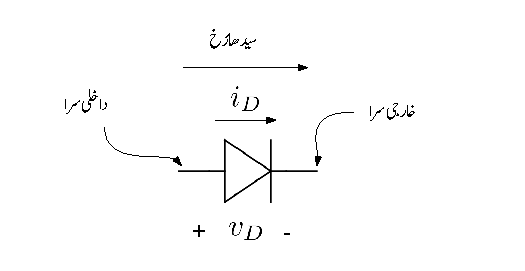
\includegraphics[scale=0.90]{diodeSymbol}
\caption{ڈایوڈ کی علامت}
\label{شکل_ڈایوڈ_کی_علامت}
\end{figure}
ڈایوڈ کے دو سروں کے مابین برقی دباو \عددی{v_D}  اور ڈایوڈ  میں سیدھے رخ  برقی رو \عددی{i_D} کو ناپنے کا درست طریقہ اسی شکل میں دکھایا گیا ہے۔ڈایوڈ کے کارکردگی کی \عددی{v_D-i_D} مساوات مندرجہ ذیل ہے۔
\begin{align}
i_D=I_S \left (e^{\frac{q v_D}{n k T}}-1 \right )
\end{align}
اس مساوات میں \موٹا{حرارتی برقی دباو}\فرہنگ{حرارتی!برقی دباو}\فرہنگ{thermal!voltage}\حاشیہب{thermal voltage} \عددی{V_T} کو
\begin{align}
V_T=\frac{k T}{q}
\end{align}
لکھتے ہوئے مساوات کو عموماً یوں لکھا جاتا ہے
\begin{align} \label{مساوات_ڈایوڈ_کی_مکمل_مساوات}
i_D=I_S \left (e^{\frac{v_D}{n V_T}}-1 \right )
\end{align}
جہاں
\begin{description}
\item
[\عددی{I_S}]  \موٹا{لبریزی برقی رو}\فرہنگ{لبریزی برقی رو}\فرہنگ{saturation!current}\حاشیہب{saturation current}
\item
[\عددی{q}]  الیکٹران کا چارج \عددی{\SI{1.6e-19}{\coulomb}}
\item
[\عددی{k}]  \موٹا{بولٹزمن}\فرہنگ{بالٹزمن کا مستقل}\فرہنگ{Boltzmann constant}\حاشیہب{Boltzmann constant} کا مستقل
  \عددی{\SI{1.38e-23}{\joule / \kelvin}}  
\item
[\عددی{T}]  \موٹا{کیلون} پیمائش حرارت\فرہنگ{کیلون پیمائش حرارت}\فرہنگ{Kelvin}\حاشیہب{Kelvin}
\item
[\عددی{V_T}] \موٹا{حرارتی برقی دباو}
\item
[\عددی{n}]  \موٹا{اخراجی جزو}\فرہنگ{اخراجی جزو}\فرہنگ{emission coefficient}\حاشیہب{emission coefficient} جس کی قیمت ایک تا دو ہوتی ہے۔مخلوط ادوار میں بنائے گئے ڈایوڈ کا عموماً \عددی{n=\num{1}} جبکہ انفرادی دو سروں والے ڈایوڈ کا \عددی{n=\num{2}} ہوتا ہے۔اس کتاب میں \عددی{n=\num{1}} تصور کیا جائے گا۔ 

\end{description}
\عددی{n=\num{1}} لیتے ہوئے
\begin{align} \label{مساوات_ڈایوڈ_کی_مساوات}
i_D=I_S \left (e^{\frac{v_D}{V_T}}-1 \right )
\end{align}
حاصل ہوتا ہے۔اس کتاب میں یہی مساوات بطور ڈایوڈ کی مساوات استعمال کی جائے گی۔

%===========
\ابتدا{مثال}
مندرجہ ذیل حرارت پر حرارتی برقی دباو \عددی{V_T}  کی قیمت حاصل کریں۔
\begin{enumerate}
\item
پانی ابلنے کے درجہ حرارت یعنی \عددی{\SI{100}{\celsius}}  پر 

\item

پانی منجمد ہونے کے درجہ حرارت یعنی \عددی{\SI{0}{\celsius}} پر
\item

تئیس ڈگری سیلسیئس یعنی \عددی{\SI{23}{\celsius}}  پر
\end{enumerate}




حل:
\begin{enumerate}
\item
پانی سو ڈگری سیلسیئس یعنی \عددی{\SI{100}{\celsius}} پر اُبلتا ہے۔اس درجہ حرارت جو کہ ڈگری سنٹی گریڈ یا ڈگری سیلسیئس \عددی{\si{\celsius}}  میں ہے کو کیلوین \عددی{\si{\kelvin}} حرارتی پیمائش میں تبدیل کرتے ہیں۔چونکہ \عددی{\si{\kelvin}=\si{\celsius}+\num{273}} ہوتا ہے لہٰذا \عددی{V_T} کی قیمت \عددی{\SI{373}{K}} پر درکار ہے۔یوں 
\begin{align*}
V_T =\frac{k T}{q} =\frac{1.38 \times 10^{-23} \times 373}{1.6 \times 10^{-19}}=\SI{0.03217}{V}
\end{align*}

\item
پانی صفر ڈگری سیلسیئس یعنی \عددی{\SI{273}{\kelvin}} پر منجمد ہوتا ہے۔اس حرارت پر
\begin{align*}
V_T=\frac{k T}{q}=\frac{1.38 \times 10^{-23} \times 273}{1.6 \times 10^{-19}}=\SI{0.0237}{V}
\end{align*}
یعنی \عددی{\SI{23.7}{\milli V}} کے برابر ہے۔
\item
تئیس ڈگری سیلسیئس جسے عام زندگی کا رہائشی درجہ حرارت لیا جاتا ہے پر حرارتی برقی دباو کی قیمت 
\begin{align*}
V_T=\frac{k T}{q}=\frac{1.38 \times 10^{-23} \times 300}{1.6 \times 10^{-19}}=\SI{0.0258}{V}
\end{align*}
یعنی  \عددی{\SI{25.8}{\milli V}} ہے۔
\end{enumerate}
عام طور ڈایوڈ کی مساوات میں حرارتی برقی دباو کو \عددی{\SI{25}{\milli V}} لیا جاتا ہے جسے یاد رکھنا قدرِ آسان ہے یعنی
\begin{align}
V_T=\SI{25}{\milli V}
\end{align}
\انتہا{مثال}
%============

\ابتدا{مثال}
ایک ایسے  ڈایوڈ جس کا \عددی{I_S=\SI{5.1} {\femto A}}  کے برابر ہو کی برقی دباو  \عددی{v_D} ان برقی رو \عددی{i_D} پر حاصل کریں۔
\begin{enumerate}
\item
$i_D=\SI{1}{\milli A}$
\item
$i_D=\SI{10}{\milli A}$
\item
$i_D=\SI{100}{\milli A}$
\end{enumerate}
حل: مساوات \حوالہ{مساوات_ڈایوڈ_کی_مکمل_مساوات}  میں  \عددی{n=1} اور \عددی{V_T=\SI{25}{\milli \volt}} لیتے ہوئے۔
\begin{enumerate}
\item
$v_D=V_T \ln \left (\frac{i_D}{I_S}+1 \right ) =0.025 \times \ln \left (\frac{1 \times 10^{-3}}{5.1 \times 10^{-15}}+1 \right ) =\SI{0.65}{V}$
\item
$v_D=V_T \ln \left (\frac{i_D}{I_S}+1 \right ) =0.025 \times \ln \left (\frac{10 \times 10^{-3}}{5.1 \times 10^{-15}}+1 \right ) =\SI{0.707}{V}$
\item
$v_D=V_T \ln \left (\frac{i_D}{I_S}+1 \right ) =0.025 \times \ln \left (\frac{100 \times 10^{-3}}{5.1 \times 10^{-15}}+1 \right ) =\SI{0.767}{V}$
\end{enumerate}
\انتہا{مثال}
%===========

مثال میں دئے ڈایوڈ سے گزرتے مثبت برقی رو\عددی{i_D}  کی قیمت  سو گنّا بڑھنے سے اس کے برقی دباو \عددی{v_D}  کی قیمت \عددی{\SI{0.65}{\volt} } سے بڑھ کر \عددی{\SI{0.767}{\volt}} ہوئی۔یہ ایک نہایت اہم اور عمومی نتیجہ ہے جسے استعمال کرتے ہم عام طور ایک ایسے سلیکان ڈایوڈ   جس میں سیدھے رُخ برقی رو کا بہاو ہو، کے دو سروں کے مابین برقی دباو کو \عددی{\SI{0.7}{\volt}}  ہی تصور کرتے ہیں یعنی
\begin{align}
v_D=\SI{0.7}{\volt}
\end{align}
یہاں بتلاتا چلوں کہ سیدھے مائل \موٹا{جرمینیم ڈایوڈ}\فرہنگ{جرمینیم ڈایوڈ}\فرہنگ{ڈایوڈ!جرمینیم}\حاشیہب{germanium diode}\فرہنگ{diode!germanium} پر \عددی{\SI{0.2}{\volt}} پائے جاتے ہیں۔  

مساوات \حوالہ{مساوات_ڈایوڈ_کی_مکمل_مساوات}  میں \عددی{I_S=\SI{5.1e-15}{\ampere}} لیتے ہوئے اسے مثبت برقی دباو کے لئے  شکل \حوالہ{شکل_ڈایوڈ_کا_خط} میں گراف کیا گیا ہے جہاں افقی محور پر \عددی{v_D} کو وولٹ میں اور عمودی محور پر \عددی{i_D} کو ایمپیئر میں دکھایا گیا ہے۔اس گراف سے واضح ہے کہ \عددی{0.5 V > v_D > 0 V}  کے احاطے میں ڈایوڈ سے گزرتی برقی رو قابلِ نظر انداز ہے۔اگرچہ جب بھی  \عددی{v_D> 0V} ہو ڈایوڈ کو \موٹا{سیدھا مائل}\فرہنگ{سیدھا مائل}\فرہنگ{مائل!سیدھا}\فرہنگ{forward biased}\حاشیہب{forward biased} تصور کیا جاتا ہے، حقیقت میں ڈایوڈ کو\عددی{v_D>0.5 V} کی صورت میں ہی \موٹا{چالو}\فرہنگ{چالو} تصور کیا جاتا ہے۔یوں \عددی{v_D=0.5 V} کو ڈایوڈ  کی \موٹا{چالو برقی دباو}\فرہنگ{چالو برقی دباو}\فرہنگ{برقی دباو!چالو}\فرہنگ{cut-in voltage}\حاشیہب{cut-in voltage}  کہتے ہیں۔چالو ڈایوڈ کی مساوات میں چونکہ 
\begin{align*}
e^{\frac{v_D}{V_T}}>>1
\end{align*}
ہوتا ہے لہٰذا چالو ڈایوڈ کی مساوات یوں لکھی جا سکتی ہے۔
\begin{align} \label{مساوات_چالو_ڈایوڈ}
i_D \approx I_S e^{\frac{v_D}{V_T}}
\end{align}
%
\begin{figure}
\centering
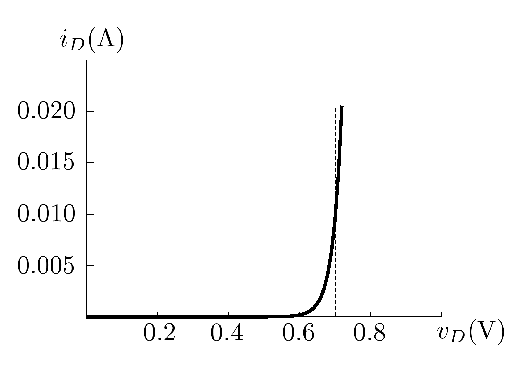
\includegraphics[scale=0.90]{diodeCharacteristics}
\caption{سیدھے مائل ڈایوڈ کا خط}
\label{شکل_ڈایوڈ_کا_خط}
\end{figure} 
شکل \حوالہ{شکل_ڈایوڈ_کا_خط} میں \عددی{\SI{0.7}{\volt}} پر نقطہ دار لکیر لگا کر اس بات کی وضاحت کی گئی ہے کہ سیدھے مائل ڈایوڈ کی برقی دباو \عددی{v_D}  تقریباً \عددی{\SI{0.7}{\volt}} وولٹ رہتی ہے۔ڈایوڈ پر سیدھے رخ برقی دباو کو \موٹا{سیدھے رخ ڈایوڈ پر برقی دباو کا گھٹاو}  کہتے ہیں جسے عموماً چھوٹا کر کے سیدھا برقی دباو کا گھٹاو یا مزید چھوٹا کر کے صرف \موٹا{سیدھا گھٹاو} کہتے ہیں۔یوں ڈایوڈ کا سیدھا گھٹاو تقریباً\عددی{\SI{0.7}{\volt}} وولٹ تصور کیا جاتا ہے۔

%=========
\ابتدا{مثال}
پچھلے مثال کے  ڈایوڈ کی برقی رو \عددی{i_D}  ان برقی دباو پر حاصل کریں۔
\begin{enumerate}
\item
$v_D=\SI{-10}{\volt}$
\item
$v_D=\SI{-1}{\volt}$
\item
$v_D=\SI{-0.1}{\volt}$
\end{enumerate}

حل:
\begin{enumerate}
\item
$
i_D=I_S \left (e^{\frac{v_D}{V_T}}-1 \right )=I_S \left (e^{-\frac{10}{0.025}} \right )=I_S \left(e^{-400}-1 \right ) \approx I_S
$
\item
$
i_D=I_S \left (e^{\frac{v_D}{V_T}}-1 \right )=I_S \left (e^{-\frac{1}{0.025}} \right ) =I_S \left (e^{-40}-1 \right ) \approx I_S
$
\item
$
i_D=I_S \left (e^{\frac{v_D}{V_T}}-1 \right )=I_S \left (e^{-\frac{0.1}{0.025}} \right ) =I_S \left (e^{-4}-1 \right ) \approx I_S
$
\end{enumerate}


\انتہا{مثال}
%============
\ابتدا{مثال}\شناخت{مثال_ڈایوڈ_الٹے_مائل_برقی_رو_لبریزی_ہے}
\عددی{I_S} کی قیمت درجہ حرارت بڑھنے  \عددی{\SI{15}{\percent}} فی کیلون بڑھتی ہے۔\عددی{\SI{5}{\celsius}} درجہ حرارت بڑھنے سے \عددی{I_S} کی قیمت کتنی ہو جائے گی۔

حل:درجہ حرارت \عددی{\SI{1}{\celsius}} بڑھنے سے نئی قیمت \عددی{1.15 I_S} ہو جائے گی۔مزید \عددی{\SI{1}{\celsius}} بڑھنے سے  \عددی{I_S} مزید \عددی{\SI{15}{\percent}} بڑھ کر \عددی{1.15 \times 1.15 I_S} یعنی \عددی{1.15^2 I_S} ہو جائے گی۔یوں \عددی{\SI{5}{\celsius}} بڑھنے سے
\begin{align*}
1.15^5 I_S \approx 2 I_S
\end{align*} 
ہو جائے گا۔
\انتہا{مثال}
%=========
اس مثال سے ہم دیکھتے ہیں کہ درجہ حرارت \عددی{\SI{5}{\celsius}} بڑھنے سے \عددی{I_S} کی قیمت دگنی ہو جاتی ہے۔اس طرح اگر مثلاً \عددی{\SI{25}{\celsius}} پر \عددی{I_S=\SI{e-15}{\ampere}} ہو تو \عددی{\SI{30}{\celsius}} پر \عددی{I_S=\SI{2e-15}{\ampere}} اور \عددی{\SI{35}{\celsius}} پر \عددی{I_S=\SI{4e-15}{\ampere}} ہو جائے گی۔
%===========
\ابتدا{مشق}
\عددی{\SI{25}{\celsius}} پر \عددی{I_S=\SI{e-15}{\ampere}}  ہے۔ \عددی{\SI{125}{\celsius}} پر \عددی{I_S} کی قیمت حاصل کریں۔

جواب:\عددی{2^{20} \times I_S \approx \SI{1}{\nano \ampere}}
\انتہا{مشق}

آپ نے مثال \حوالہ{مثال_ڈایوڈ_الٹے_مائل_برقی_رو_لبریزی_ہے} میں دیکھا کہ منفی \عددی{v_D} کی صورت میں برقی رو کی قیمت   تقریباً \عددی{-I_S} کے برابر ہوتی ہے یعنی برقی رو کا بہاو ڈایوڈ میں اُلٹی رُخ کی جانب ہوتا ہے جبکہ اس کا کل مقدار \عددی{\abs{I_S}} رہتا ہے۔یاد رہے کہ \عددی{I_S} ایک نہایت چھوٹی مقدار ہے جسے عموماً صفر ہی تصور کیا جاتا ہے۔حقیقی ڈایوڈ میں الٹے رخ برقی رو کی قیمت  \عددی{I_S} سے کئی درجہ زیادہ ہوتی ہے۔مثلاً جہاں الٹے مائل ڈایوڈ کے مساوات کے مطابق \عددی{I_S=\SI{e-15}{\ampere}} برقی رو گزرنا چاہئے وہاں حقیقت میں الٹے رخ \عددی{\SI{e-9}{\ampere}} برقی رو بھی ممکن ہے۔مزید یہ کہ الٹا مائل کرنے والا برقی دباو بھی الٹے رخ برقی رو کی مقدار  پر اثر انداز ہوتا ہے۔

الٹے رخ برقی رو کا بیشتر حصہ ڈایوڈ میں \موٹا{الٹے رخ رستا برقی رو}\فرہنگ{الٹی رستا برقی رو}\فرہنگ{برقی رو!الٹی رستا}\فرہنگ{reverse leakage current}\حاشیہب{reverse leakage current}  ہے جو ڈایوڈ کے \عددی{pn} جوڑ کے رقبے کے ساتھ راہ راست تناسب رکھتا ہے۔\عددی{I_S} بھی ڈایوڈ کے \عددی{pn} جوڑ کے رقبے کے ساتھ راہ راست تناسب رکھتا  ہے۔درجہ حرارت \عددی{\SI{5}{\celsius}} بڑھنے سے\عددی{I_S} کی قیمت دگنا ہو جاتی ہے جبکہ  \موٹا{الٹے رخ رستا برقی رو} کی قیمت  \عددی{\SI{10}{\celsius}} بڑھنے سے دگنا ہوتی ہے۔


جب ڈایوڈ پر بیرونی لاگو برقی دباو ڈایوڈ میں الٹے رخ برقی رو گزارنے کی کوشش کرے ہم کہتے ہیں کہ ڈایوڈ  \موٹا{الٹا مائل}\فرہنگ{مائل!الٹا}\فرہنگ{reverse biased}\حاشیہب{reverse biased}  کیا گیا ہے اور اسی طرح بیرونی لاگو برقی دباو ڈایوڈ میں سیدھے رخ برقی رو گزارنے کی کوشش کرے تب ہم کہتے ہیں کہ ڈایوڈ \موٹا{سیدھا مائل}\فرہنگ{سیدھا مائل}\فرہنگ{مائل!سیدھا}\فرہنگ{forward biased}\حاشیہب{forward biased} کیا گیا ہے۔
\begin{figure}
\centering
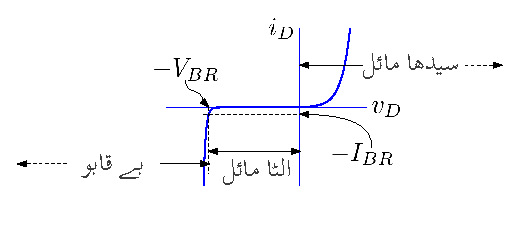
\includegraphics[scale=0.90]{diodeVIcurve}
\caption{ڈایوڈ کا برقی دباو بالمقابل برقی رو کا خط}
\label{شکل_ڈایوڈ_برقی_دباو_بالمقابل_برقی_رو}
\end{figure}
شکل \حوالہ{شکل_ڈایوڈ_برقی_دباو_بالمقابل_برقی_رو}  میں ڈایوڈ کا برقی دباو بالمقابل برقی رو \عددی{(v_D-i_D)} کا خط دکھایا گیا ہے جس میں ڈایوڈ کے سیدھے مائل اور الٹے مائل خطے دکھائے گئے ہیں۔اس شکل میں \موٹا{بے قابو خطہ}\فرہنگ{بے قابو خطہ}\فرہنگ{breakdown region}\حاشیہب{breakdown region} بھی دکھایا گیا ہے جو مساوات \حوالہ{مساوات_ڈایوڈ_کی_مکمل_مساوات}  سے کسی صورت اخذ نہیں کیا جا سکتا۔

دراصل مساوات \حوالہ{مساوات_ڈایوڈ_کی_مکمل_مساوات}  حاصل کرتے وقت ڈایوڈ کی کئی پیچیدگیاں نظر انداز کی گئیں اور یوں اگرچہ یہ مساوات سیدھے مائل ڈایوڈ کی کارکردگی کو بہت بہتر بیان کرتا ہے، الٹے مائل ڈایوڈ کی کارکردگی کو یہ پوری طرح صحیح بیان نہیں کرتا اور ڈایوڈ کے بے قابو خطے کو سراسر خطا کر جاتا ہے۔بے قابو خطے پر آگے تبصرہ کیا جائے گا۔یہاں صرف اتنا بتانا ضروری ہے کہ اگر ڈایوڈ پر الٹے رخ برقی دباو لاگو کر کے اسے الٹا مائل کیا جائے تو ڈایوڈ اس برقی دباو کو برداشت کرتا ہے اور الٹے رخ برقی رو نہیں گزرنے دیتا۔اگر اس الٹا مائل کرنے والے برقی دباو کو بتدریج بڑھائی جائے تو آخر کار یہ ڈایوڈ کے برداشت کے حد سے تجاوز کر جائے گا اور ڈایوڈ یک دم الٹے رخ بے قابو برقی رو گزارنے دے گا۔جس برقی دباو پر ایسا ہو اسے ڈایوڈ کی  \موٹا{ناقابلِ برداشت الٹ برقی دباو}\فرہنگ{ناقابل برداشت الٹ برقی دباو}\فرہنگ{reverse breakdown voltage}\حاشیہب{reverse breakdown voltage} \عددی{V_{BR}}   کہتے ہیں۔اگرچہ گراف میں ناقابلِ برداشت برقی دباو منفی محور پر ہے، اس کی قیمت مثبت لکھی اور پڑھی جاتی ہے۔مختلف ڈایوڈ کی ناقابل برداشت برقی دباو مختلف ہوتی ہے اور یہ چند وولٹ سے ہزاروں وولٹ تک ممکن ہے۔


شکل \حوالہ{شکل_ڈایوڈ_برقی_دباو_بالمقابل_برقی_رو} میں دکھائے تین خطوں کی نشاندہی یوں کی جاتی ہے۔
\begin{itemize}
\item
سیدھا مائل  \عددی{0 < v_D}
\item
الٹا مائل \عددی{-V_{BR}< v_D < 0}
\item
بے قابو \عددی{v_D < -V_{BR}}
\end{itemize}
ڈایوڈ کی مساوات میں \عددی{V_T} واضح طور پر درجہ حرارت پر منحصر ہے۔اگرچہ\عددی{I_S} کو مستقل سمجھا گیا ہے،حقیقت میں یہ بھی درجہ حرارت پر منحصر ہوتا ہے۔اگر ڈایوڈ میں سیدھے رخ برقی رو کی قیمت تبدیل نہ کرتے ہوئے درجہ حرارت بڑھایا جائے تو مساوات \حوالہ{مساوات_ڈایوڈ_کی_مکمل_مساوات}  میں\عددی{V_T} کی وجہ سے ہم توقع کرتے ہیں کہ ڈایوڈ پر برقی دباو کی قیمت بھی بڑھے گی۔جیسا شکل \حوالہ{شکل_برقی_دباو_بالمقابل_حرارت}  میں دکھایا گیا ہے،حقیقت میں ایسا نہیں ہوتا اور ہم دیکھتے ہیں کہ برقی رو بدلے بغیر،  \عددی{\SI{1}{\celsius}} درجہ حرارت بڑھانے سے ڈایوڈ پر برقی دباو کی قیمت \عددی{\SI{2}{\milli \volt}} گھٹتی ہے۔دراصل درجہ حرارت بڑھانے سے \عددی{I_S} کی قیمت بھی بڑھتی ہے اور \عددی{I_S}  کا اثر\عددی{V_T} کے اثر پر غالب ہے۔مزید یہ کہ حقیقت میں الٹے رخ برقی رو کی مقدار الٹے رخ برقی دباو کی قیمت بڑھانے سے معمولی بڑھتی ہے۔درجہ حرارت کے ساتھ ڈایوڈ پر برقی دباو کی قیمت کی تبدیلی کو برقیاتی \موٹا{تھرمامیٹر}\فرہنگ{تھرمامیٹر}\فرہنگ{thermometer}\حاشیہب{thermometer} بنانے میں بروئے کار لایا گیا ہے۔

\begin{figure}
\centering
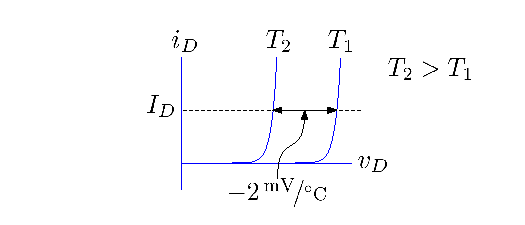
\includegraphics[scale=0.90]{diodeVoltageVersusTemperature}
\caption{برقی دباو بالمقابل درجہ حرارت}
\label{شکل_برقی_دباو_بالمقابل_حرارت}
\end{figure}

\ابتدا{مثال}
میں نے لاہور میں ٹھوکر نیاز بیگ کے مقام پر واقع \موٹا{عطا گروپ آف انڈسٹریز}\حاشیہب{Atta group of industries} میں کام کرتے ہوئے \موٹا{قوی برقیات}\حاشیہب{power electronics} کے میدان میں \عددی{\SI{100}{\kilo \watt}} تا \عددی{\SI{1.5}{\mega \watt}} کے  لوہا پگھالنے کی بھٹیاں\حاشیہب{induction furnaces} بنائیں۔ قوی برقیات میں ہزاروں ایمپیئر اور وولٹ کے صلاحیت رکھنے والے ڈایوڈ استعمال کئے جاتے ہیں۔یہ مثال مجھے اُس وقت درپیش مسائل میں سے لیا گیا ہے۔
 
ایک ڈایوڈ میں یکدم \عددی{\SI{1000}{\ampere}} گزارنے سے اس پر شروع میں \عددی{V_D=\SI{0.724}{\volt}} پائے جاتے ہیں جو کچھ دیر میں گھٹتے ہوئے \عددی{\SI{0.708}{\volt}} ہو کر اسی قیمت پر برقرار رہتے ہیں۔
\begin{itemize}
\item
برقی رو گزرنے سے ڈایوڈ کی اندرونی درجہ حرارت میں کتنا اضافہ پیدا ہوا۔
\item
گرم ہونے کے بعد ڈایوڈ میں برقی طاقت کا ضیاع حاصل کریں۔
\item
فی واٹ طاقت کے ضیاع سے درجہ حرارت میں اضافے کو ڈایوڈ کا \موٹا{حرارتی مزاحمت}\فرہنگ{حرارتی!مزاحمت}\فرہنگ{thermal!resistance}\حاشیہب{thermal resistance} کہتے ہیں۔ڈایوڈ کا \موٹا{حرارتی مزاحمت} حاصل کریں۔
\end{itemize}

حل:
\begin{itemize}
\item
 \عددی{V_D} میں \عددی{0.708-0.724} یعنی \عددی{\SI{-0.016}{\volt}} کی تبدیلی پیدا ہوئی۔چونکہ \عددی{\SI{1}{\celsius}} درجہ حرارت بڑھنے سے \عددی{V_D} میں \عددی{\SI{-2}{\milli \volt}} کی تبدیلی رونما ہوتی ہے لہٰذا ڈایوڈ کے اندرونی درجہ حرارت میں \عددی{\tfrac{0.016}{0.002}} یعنی \عددی{\SI{8}{\celsius}} کا اضافہ پیدا ہوا۔
\item
ڈایوڈ میں برقی طاقت کا ضیاع \عددی{1000 \times 0.708=\SI{708}{\watt}} ہے۔
\item
\موٹا{حرارتی مزاحمت} \عددی{\tfrac{8}{708}=\SI{0.011}{\celsius \per \watt}} ہے۔
\end{itemize}
\انتہا{مثال}

\حصہ{کامل ڈایوڈ}  
	ڈایوڈ   سمجھنے کی خاطر ہم کامل ڈایوڈ  کی بات کرتے ہیں۔کامل ڈایوڈ\حاشیہب{ideal diode}  حقیقت میں نہیں پایا جاتا مگر اسے سمجھنا آسان اور اسے سمجھ کر اصل ڈایوڈ   کی کارکردگی سمجھنا زیادہ آسان ہوتا ہے۔

ڈایوڈ   کی کارکردگی دِل کے والو\حاشیہب{valve}  کی مانند ہے۔دِل کا والو خون کو صرف ایک جانب گزرنے دیتا ہے۔اسی طرح ڈایوڈ   برقی رو کو صرف سیدھے رُخ گزرنے دیتا ہے۔شکل \حوالہ{شکل_پانی_کا_والو}  میں پانی کے پائپ پر نسب والو دکھایا گیا ہے جس کی کارکردگی شکل سے ہی واضح ہے۔

\begin{figure}
\centering
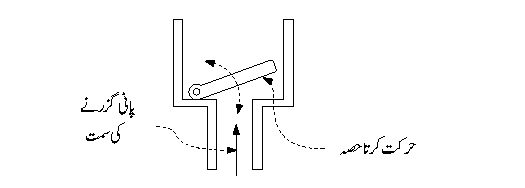
\includegraphics[scale=0.90]{diodeAsValve}
\caption{پانی کے پائپ پر نسب والو}
\label{شکل_پانی_کا_والو}
\end{figure}

برقی نقطہ نظر سے کامل ڈایوڈ   کو ایک ایسا خود کار برقی \موٹا{سوئچ}\حاشیہب{switch} تصور کیا جا سکتا ہے جو ڈایوڈ میں سے گزرتی برقی رو کی سمت کو دیکھتے ہوئے \موٹا{چالو}\فرہنگ{switch ON}  یا منقطع\حاشیہب{switch OFF}  ہو سکے۔ڈایوڈ   میں سیدھے رخ برقی رو اسے چالو کرتی ہے جبکہ اُلٹ رُخ برقی رو اسے منقطع کرتی ہے۔یوں  ڈایوڈ میں اُلٹی رُخ برقی رو کا گزر ممکن نہیں ہوتا۔شکل \حوالہ{شکل_ڈایوڈ_بطور_برقی_سوئچ}  میں ایسا دکھایا گیا ہے۔اس سوئچ کا خط شکل \حوالہ{شکل_ڈایوڈ_سوئچ_کا_خط} میں دکھایا گیا ہے۔اس شکل کا ڈایوڈ کے خط کے ساتھ موازنہ کریں۔اگر  ڈایوڈ کے \عددی{\SI{0.7}{\volt}}  کو نظر انداز کیا جائے تو یہ دونوں خطوط یکساں معلوم ہوتے ہیں

\begin{figure}
\centering
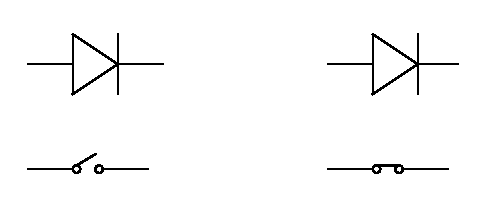
\includegraphics[scale=0.90]{diodeAsSwitch}
\caption{ڈایوڈ بطور برقی سوئچ}
\label{شکل_ڈایوڈ_بطور_برقی_سوئچ}
\end{figure}


\begin{figure}
\centering
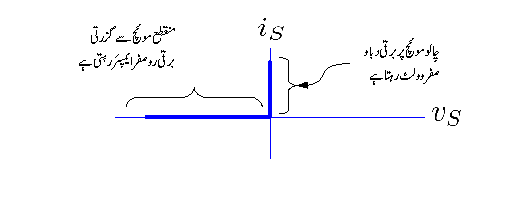
\includegraphics[scale=0.90]{diodeSwitchCharacteristics}
\caption{ڈایوڈ سوئچ کا خط}
\label{شکل_ڈایوڈ_سوئچ_کا_خط}
\end{figure}
\حصہ{ڈایوڈ   کے چند ادوار}
	شکل \حوالہ{شکل_ڈایوڈ_سیدھا_مائل_الٹا_مائل}  میں تین ادوار دکھائے گئے ہیں۔شکل  الف میں برقی دباو \عددیء{v_I}، گھڑی کی سمت میں برقی رو \عددی{i} پیدا کرتا ہے جسے تیر کے نشان سے ظاہر کیا گیا ہے۔شکل  ب اور شکل  پ میں مزاحمت کے ساتھ سلسلہ وار ڈایوڈ   بھی نسب کر دئے گئے ہیں۔شکل  ب میں ڈایوڈ   یوں جوڑا گیا ہے کہ برقی رو \عددی{i} کی سمت شکل \حوالہ{شکل_ڈایوڈ_کی_علامت}  میں دکھائے ڈایوڈ کے سیدھے رخ کی جانب ہے جبکہ شکل  پ میں برقی رو\عددی{i} کی سمت ڈایوڈ کی اُلٹ رخ کی جانب ہے۔یوں شکل  ب میں برقی رو \عددی{i} کا گزر ممکن ہے جبکہ شکل  پ میں برقی رو \عددی{i} کا گزر ناممکن ہے۔
\begin{figure}
\centering
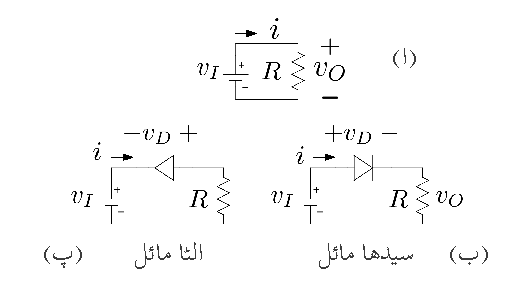
\includegraphics[scale=0.90]{diodeForwardReverseBiased}
\caption{سیدھا مائل ڈایوڈ اور الٹا مائل ڈایوڈ}
\label{شکل_ڈایوڈ_سیدھا_مائل_الٹا_مائل}
\end{figure}
شکل  ب میں برقی دباو \عددی{v_I} ڈایوڈ   کو مائل کرتا ہے کہ یہ برقی رو کو سیدھے رُخ گزرنے دے۔ہم کہتے ہیں کہ ڈایوڈ   \موٹا{سیدھے رُخ مائل}  کیا گیا ہے یا کہ ڈایوڈ   \موٹا{سیدھا مائل}\فرہنگ{سیدھا مائل}\فرہنگ{forward biased}\حاشیہب{forward biased} کیا گیا ہے۔اس کے برعکس شکل  پ میں برقی دباو \عددی{v_I} ڈایوڈ   میں اُلٹے رُخ برقی رو گزارنے کی کوشش کرتا ہے۔اس صورت میں ہم کہتے ہیں کہ ڈایوڈ   \موٹا{اُلٹے رُخ مائل}  کیا گیا ہے یا کہ ڈایوڈ   \موٹا{اُلٹا مائل}\فرہنگ{الٹا!مائل}\فرہنگ{reverse biased}\حاشیہب{reverse biased} کیا گیا ہے۔ ڈایوڈ کے سیدھے مائل حال کو \موٹا{چالو حال} جبکہ اس کے اُلٹ مائل حال کو \موٹا{منقطع حال} بھی کہتے ہیں۔ 
	شکل  ب کے لئے کرچاف  کی مساوات برائے برقی دباو لکھتے ہیں۔
\begin{align} \label{مساوات_ڈایوڈ_سیدھا_مائل_مثال_الف}
v_I=v_D+i R
\end{align}


%==========
\ابتدا{مثال}
شکل \حوالہ{شکل_ڈایوڈ_سیدھا_مائل_الٹا_مائل} ب میں مزاحمت کی قیمت \عددی{\SI{1}{\kilo \ohm}} تصور کریں۔ ڈایوڈ کے برقی دباو \عددی{v_D} کو پہلے نظر انداز کرتے ہوئے اور بعد میں اسے\عددی{\SI{0.7}{\volt}}  لیتے ہوئے مندرجہ ذیل صورتوں میں برقی رو حاصل کریں۔
\begin{enumerate}
\item
$v_I=\SI{22.9}{\volt}$
\item
$v_I=\SI{1.2}{\volt}$
\end{enumerate}

حل:	\عددی{v_D} کو نظر انداز کرتے ہوئے مساوات \حوالہ{مساوات_ڈایوڈ_سیدھا_مائل_مثال_الف}  کی مدد سے حل کرتے ہیں۔
\begin{enumerate}
\item
$i=\frac{v_I}{R}=\frac{22.9}{1000}=\SI{22.9}{\milli \ampere}$
\item
$i=\frac{v_I}{R}=\frac{1.2}{1000}=\SI{1.2}{\milli \ampere}$
\end{enumerate}
اب \عددی{v_D=\SI{0.7}{\volt}} لیتے ہوئے دوبارہ حل کرتے ہیں۔
\begin{enumerate}
\item
$i=\frac{v_I}{R}=\frac{22.9-0.7}{1000}=\SI{22.2}{\milli \ampere}$
\item
$i=\frac{v_I}{R}=\frac{1.2-0.7}{1000}=\SI{0.5}{\milli \ampere}$
\end{enumerate}

\انتہا{مثال}
%================

اس مثال میں \عددی{v_I=\SI{22.9 }{\volt}} کی صورت میں \عددی{v_D} کے اثر کو شامل کرنے سے حاصل برقی رو \عددی{i}  کی قیمت پر خاطر خواہ اثر نہیں پڑتا جبکہ\عددی{v_I=\SI{1.2}{\volt}} کی صورت میں اس کے شمولیت سے برقی رو کی قیمت آدھے سے بھی کم ہو جاتی ہے۔اس سے ظاہر ہوتا ہے کہ \عددی{v_D} کو ہر جگہ نظرانداز نہیں کیا جا سکتا۔

\حصہ{بدلتی دباو سے یک سمتی دباو کا حصول (سمت کاری)}
 
\جزوحصہ{نصف لہر سمت کاری}
	شکل \حوالہ{شکل_نصف_لہر_مثبت_سمت_کار}  میں بدلتی داخلی برقی دباو \عددی{v_i = V_p \sin \omega t}  کے مثبت حصے ڈایوڈ  کو سیدھا مائل کرتے ہیں۔یوں اس دوران
\begin{align*}
v_o = v_i  - v_D \approx V_p \sin \omega t  - 0.7
\end{align*}
ہوتا ہے جہاں سیدھے مائل ڈایوڈ پر برقی دباو کو تقریباً \عددی{\SI{0.7}{\volt}} لیا گیا ہے۔اس کے برعکس \عددی{v_i}  کے منفی حصے ڈایوڈ کو اُلٹا مائل کر کے منقطع کر دیتے ہیں اور یوں اس دوران  \عددی{v_o = \SI{0}{\volt}} ہوتا ہے۔
\begin{figure}
\centering
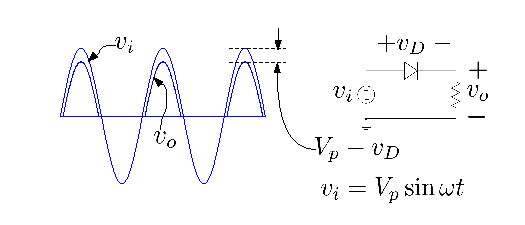
\includegraphics[scale=0.90]{halfWaveRectifierPositive}
\caption{نصف لہر مثبت سمت کار}
\label{شکل_نصف_لہر_مثبت_سمت_کار}
\end{figure}
شکل \حوالہ{شکل_نصف_لہر_مثبت_سمت_کار} میں  \عددی{v_i} اور \عددی{v_o} بھی گراف کئے گئے ہیں۔آپ دیکھ سکتے ہیں کہ \عددی{v_o}  کی چوٹی \عددی{v_i} کے چوٹی سے تقریباً \عددی{\SI{0.7}{\volt}} کم ہے۔عمومی استعمال میں \عددی{v_i} کی چوٹی کی قیمت \عددی{\SI{0.7}{\volt}} سے گئی گنّا زیادہ ہوتی ہے اور یوں \عددی{v_o} کے چوٹی کو \عددی{v_i} چوٹی کے برابر ہی تصور کیا جاتا ہے۔

اس دور کی مدد سے بدلتی داخلی برقی دباو جو مثبت اور منفی حصوں پر مشتمل ہے سے ایک ایسی خارجی برقی دباو حاصل کی گئی ہے جس میں داخلی برقی دباو کے صرف مثبت حصے موجود ہیں۔ بدلتی برقی دباو سے نصف لہر کی یک سمتی برقی دباو کے حصول کو \موٹا{نصف لہر سمت کاری}\حاشیہب{half wave rectification}  کہتے ہیں۔یوں شکل \حوالہ{شکل_نصف_لہر_مثبت_سمت_کار} میں دئے دور کو \قریب{\موٹا{نصف لہر مثبت سمت کار}}\فرہنگ{نصف لہر!مثبت سمت کار}\فرہنگ{سمت کار!نصف لہر}\فرہنگ{half wave rectifier!positive}\حاشیہب{half wave positive rectifier}  کہتے ہیں۔

نصف سمت کار جسے عام فہم میں \موٹا{آدھا ریکٹیفائر}\حاشیہب{half wave rectifier} کہتے ہیں ایک انتہائی اہم دور ہے جسے استعمال کرتے ہوئے کئی ادوار مثلاً \موٹا{پیدا کار برقی دباو} یعنی برقی دباو کی \موٹا{سپلائی}\فرہنگ{برقی دباو سپلائی}\فرہنگ{power supply} ، بیٹری چارجر\حاشیہد{موبائل فون رکھنے والے بیٹری چارجر سے بخوبی آگاہ ہوں گے۔} وغیرہ بنائے جاتے ہیں۔
\begin{figure}
\centering
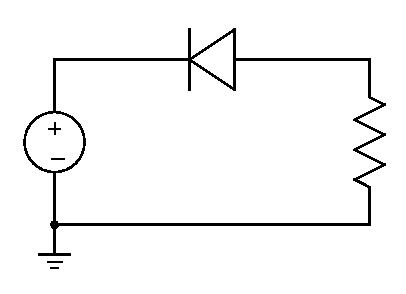
\includegraphics[scale=0.90]{halfWaveRectifierNegative}
\caption{نصف لہر منفی سمت کار}
\label{شکل_نصف_لہر_منفی_سمت_کار}
\end{figure}
شکل \حوالہ{شکل_نصف_لہر_منفی_سمت_کار} میں ڈایوڈ کو قدرِ مختلف طریقہ سے جوڑا گیا ہے۔اس صورت میں داخلی برقی دباو \عددی{v_i} کے منفی حصے ڈایوڈ کو سیدھا مائل کرتے ہیں جبکہ اس کے مثبت حصے ڈایوڈ کو اُلٹا مائل کرتے ہیں۔یوں خارجی برقی دباو میں داخلی برقی دباو کے صرف منفی حصے موجود ہوتے ہیں۔اس دور کو \قریب{\موٹا{نصف لہر منفی سمت کار}}\فرہنگ{نصف لہر!منفی سمت کار}\فرہنگ{half wave rectifier!negative}\حاشیہب{half wave negative rectifier} کہتے ہیں۔
%==============
\ابتدا{مثال}\شناخت{مثال_نصف_لہر_سمتکار_مستطیل_داخلی_دباو}
بار سے لدے مثبت نصف لہر سمت کار کو \عددی{\SI{50}{\hertz}} تعدد \عددی{\SI{\mp15}{\volt}} حیطے کا مستطیل داخلی اشارہ فراہم کیا جاتا ہے جس کے مثبت اور منفی حصے برابر دورانیہ کے ہیں۔بار \عددی{R_L=\SI{100}{\ohm}} جبکہ \عددی{C=\SI{100}{\micro \farad}} ہیں۔خارجی برقی دباو بلدار ہوتا ہے۔اس میں \موٹا{بل}\فرہنگ{بل}\فرہنگ{ripple}\حاشیہب{ripple} کی مقدار حاصل کریں۔ڈایوڈ پر برقی دباو کے گھٹنے کو نظر انداز کریں۔خارجی برقی دباو میں \موٹا{بل} کو \عددی{\SI{1}{\volt}} سے کم رکھنے کی خاطر درکار کپیسٹر کی قیمت حاصل کریں۔
\begin{figure}
\centering
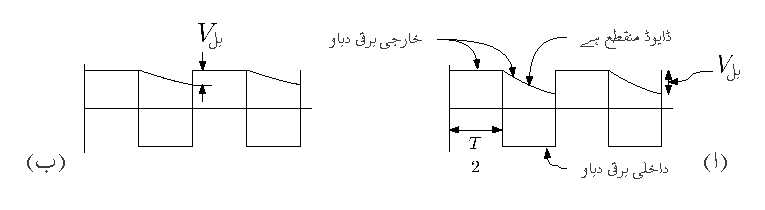
\includegraphics[scale=0.90]{halfWaveRectifierSquareInput}
\caption{نصف لہر سمت کار کے خارجی برقی دباو میں بل}
\label{شکل_نصف_لہر_سمتکار_بل}
\end{figure}
حل:
شکل \حوالہ{شکل_نصف_لہر_سمتکار_بل} الف میں صورت حال دکھائی گئی ہے جہاں خارجی برقی دباو کا \موٹا{بلدار} ہونا واضح ہے۔داخلی برقی دباو منفی ہونے کے صورت میں ڈایوڈ منقطع رہتا ہے۔اس دوران کپیسٹر \عددی{C} برقی طاقت فراہم کرتا ہے۔پچاس تعدد کے اشارے کا \موٹا{دوری عرصہ}\حاشیہب{time period} بیس ملی سیکنڈ ہے۔یوں کپیسٹر سے دس ملی سیکنڈ کے لئے چارج کی نکاسی ہوتی ہے۔داخلی برقی دباو کے منفی ہونے کے لمحے کو \عددی{t=0} لیتے ہوئے کپیسٹر پر برقی دباو \عددی{v_C} کو یوں لکھا جا سکتا ہے
\begin{align*}
v_C=V_p e^{-\frac{t}{RC}}
\end{align*}
جہاں \عددی{V_p=\SI{15}{\volt}} ہے۔اس مساوات سے دس ملی سیکنڈ بعد \عددی{v_C=\SI{5.5}{\volt}} حاصل ہوتا ہے جس سے
\begin{align*}
V_{\textrm{بل}}=15-5.5=\SI{9.5}{\volt}
\end{align*}
حاصل ہوتا ہے۔

بل کو \عددی{\SI{1}{\volt}} رکھنے کی خاطر دس ملی سیکنڈ نکاسی کے بعد \عددی{v_C=15-1=14} درکار ہے۔یوں
\begin{align*}
14=15 e^{-\frac{0.01}{100 C}}\\
C=\SI{1449}{\micro \farad}
\end{align*}
حاصل ہوتا ہے۔کپیسٹر، مزاحمت وغیرہ متعین قیمتوں میں دستیاب ہوتے ہیں لہٰذا انہیں قیمتوں میں سے کپیسٹر، مزاحمت وغیرہ چنا ہوتا ہے۔ہم \عددی{\SI{1500}{\micro \farad}} اور \عددی{\SI{25}{\volt}} کا کپیسٹر استعمال کریں گے۔کپیسٹر کے برقی دباو کی صلاحیت درکار برقی دباو کی چوٹی سے زیادہ ہونا لازمی ہے۔ 

آپ نے دیکھا کہ کپیسٹر کی قیمت بڑھانے سے \موٹا{بل} میں کمی آتی ہوتی ہے۔یہ حقیقت برقی دباو کے \موٹا{سپلائی}\حاشیہب{voltage supply} میں کام آئے گی۔
\انتہا{مثال}
%=========
\ابتدا{مثال}
شکل \حوالہ{شکل_بیٹری_چارجر}-ا میں نصف لہر مثبت سمت کار کے خارجی جانب مزاحمت کی جگہ  بیٹری نسب کی گئی ہے۔یوں نصف لہر کار بیٹری چارج کرتا ہے۔اس دور میں بیٹری کا برقی دباو \عددی{V_B=\SI{12}{\volt}} جبکہ \عددی{R=\SI{100}{\ohm}} اور \عددی{v_i = 15 \sin \omega t} ہے جہاں \عددی{\omega = 100 \pi} کے برابر ہے۔اس بیٹری چارجر کی برقی رو \عددی{i_B} حاصل کر کے گراف کریں۔مزاحمت \عددی{R} برقی رو کی چوٹی کو ڈایوڈ اور بیٹری کے قابلِ برداشت حد سے نیچے رکھتا ہے۔
\begin{figure}
\centering
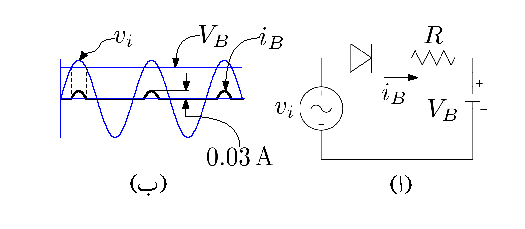
\includegraphics[scale=0.90]{batteryCharger}
\caption{بیٹری چارجر}
\label{شکل_بیٹری_چارجر}
\end{figure}
حل:	داخلی برقی دباو \عددی{v_i} کی قیمت مسلسل تبدیل ہوتا ہے۔جب تک \عددی{v_i} کی قیمت بیٹری کے برقی دباو یعنی بارہ وولٹ سے کم رہے ڈایوڈ الٹا مائل رہے گا اور اس میں برقی رو نہیں گزرے گی۔جیسے ہی \عددی{v_i} کی قیمت  \عددی{\SI{+12}{\volt}} سے تجاوز کرے ڈایوڈ سیدھا مائل ہو کر برقی رو گزارے گا اور اس دوران \عددی{v_D}  کو نظر انداز کرتے ہوئے مزاحمت پر  اُوہم کے قانون سے ہم لکھ سکتے ہیں۔
\begin{align*}
i_R=i_B=\frac{v_i-V_B}{R}=\frac{15 \sin 100 \pi t -12 }{100}=0.15 \sin  100 \pi t -0.12
\end{align*}

شکل \حوالہ{شکل_بیٹری_چارجر}  - ب میں بیٹری چارج کرنے والی برقی رو \عددی{i_B} کے علاوہ \عددی{v_i} اور \عددی{V_B} بھی دکھائے گئے ہیں۔برقی دباو اور برقی رو کو ایک ہی جگہ گراف کیا گیا ہے تا کہ وقت \عددی{t} کے ساتھ مختلف متغیرات کے تعلق کی وضاحت ہو سکے۔ جیسا آپ دیکھ سکتے ہیں بیٹری صرف ان اوقات چارج ہوتا ہے جب \عددی{v_i > V_B} ہو۔شکل میں نقطہ دار لکیروں سے ایسے ایک دورانیہ کی نشاندہی کی گئی ہے  جب بیٹری چارج ہو رہی ہو۔کی چوٹی \عددی{\SI{30}{\milli \ampere}} ہے جسے  یوں حاصل کیا گیا۔
\begin{align*}
0.15 \sin \frac{\pi}{2}-0.12=0.15-0.12=\SI{0.03}{\ampere}
\end{align*}

\انتہا{مثال}
%===========


\جزوحصہ{مکمل لہر سمت کاری}
شکل \حوالہ{شکل_مکمل_لہر_سمت_کار} میں \موٹا{مکمل لہر سمت کار}\فرہنگ{مکمل لہر سمت کار}\فرہنگ{سمت کار!مکمل لہر}\فرہنگ{full wave rectifier}\حاشیہب{full wave rectifier} دکھایا گیا ہے۔اس دور میں چار ڈایوڈ مربع کی شکل میں جوڑے گئے ہیں اور دور کو \عددی{v_i} بطور بدلتا داخلی برقی دباو مہیا کیا گیا ہے۔دور کی کارکردگی سمجھنے کی خاطر شکل \حوالہ{شکل_مکمل_لہر_سمت_کار_کے_خط} الف  پر توجہ رکھیں۔\عددی{v_i} کی قیمت مثبت ہونے کی صورت میں پیدا کار برقی دباو کے مثبت \عددی{(+)}  سرے سے برقی رو باہر کی جانب ہو گی۔چونکہ برقی رو ڈایوڈ میں الٹی جانب نہیں گزر سکتی لہٰذا یہ ڈایوڈ \عددی{D_2} سے گزرے گی جبکہ اس دوران ڈایوڈ \عددی{D_4} منقطع حال رہے گا۔برقی رو \عددی{D_2} سے خارج ہو کر چونکہ \عددی{D_1} میں الٹی جانب نہیں گزر سکتی لہٰذا یہ مزاحمت \عددی{R} میں داخل ہو گی۔

اسی طرح پیدا کار برقی دباو کے منفی سرے سے برقی رو کی راہ معلوم کرنے کی خاطر ہم دیکھتے ہیں کہ پیدا کار برقی دباو کے منفی \عددی{(-)} سرے پر برقی رو اندر کی جانب ہو گی۔یہ برقی رو صرف \عددی{D_3} کے راستے ہی ممکن ہے چونکہ \عددی{D_1} میں الٹی برقی رو کا گزر ناممکن ہے۔
\begin{figure}
\centering
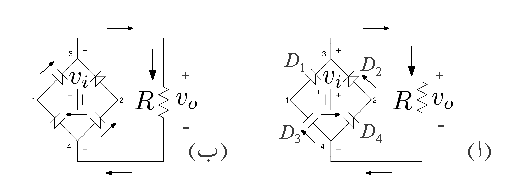
\includegraphics[scale=0.90]{fullWaveRectifier}
\caption{مکمل لہر سمت کار}
\label{شکل_مکمل_لہر_سمت_کار}
\end{figure}
ہم دیکھتے ہیں کہ مثبت برقی دباو کی صورت میں برقی رو ڈایوڈ  \عددی{D_2} اور  \عددی{D_4} سے گزرتی ہے جبکہ ڈایوڈ  \عددی{D_1} اور  \عددی{D_3} منقطع رہتے ہیں۔اس دوران مزاحمت میں برقی رو کی سمت شکل میں دکھائی گئی ہے۔

اب دیکھتے ہیں کہ پیدا کار برقی دباو کے برقی دباو کی قیمت منفی ہونے کی صورت میں کیا ہوتا ہے۔یہ صورتِ حال شکل \حوالہ{شکل_مکمل_لہر_سمت_کار} - ب میں دکھائی گئی ہے۔اس صورت میں برقی رو ڈایوڈ  \عددی{D_1} اور \عددی{D_4} سے گزرے گی جبکہ  \عددی{D_2} اور  \عددی{D_3} منقطع رہیں گے۔برقی رو اب بھی مزاحمت میں گزشتہ سمت میں ہی گزرے گی۔

یوں جیسا شکل \حوالہ{شکل_مکمل_لہر_سمت_کار_کے_خط}  میں دکھایا گیا ہے، بدلتے داخلی دباو \عددی{v_i} کی قیمت مثبت یا منفی ہو، مزاحمت پر ہر وقت برقی دباو \عددی{v_o}مثبت ہی رہتا ہے۔ چونکہ \عددی{v_o} کی سمت تبدیل نہیں ہوتی لہٰذا یہ یک سمتی برقی دباو ہے۔
\begin{figure}
\centering
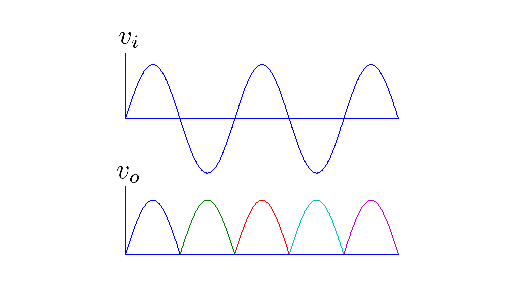
\includegraphics[scale=0.90]{fullWaveRectifierOutputWave}
\caption{مکمل لہر سمت کار کے داخلی اور خارجی خط}
\label{شکل_مکمل_لہر_سمت_کار_کے_خط}
\end{figure}

\حصہ{چوٹی حاصل کار} \شناخت{حصہ_چوٹی_حاصل_کار}
	شکل \حوالہ{شکل_چوٹی_حاصل_کار}  میں \موٹا{چوٹی حاصل کار}\فرہنگ{چوٹی حاصل کار}\فرہنگ{peak detector}\حاشیہب{peak detector} دکھایا گیا ہے۔اس دور کو مثبت آدھے لہر سمت کار میں ڈایوڈ   کے خارجی جانب مزاحمت کی جگہ کپیسٹر نسب کر کے حاصل کیا گیا ہے۔
\begin{figure}
\centering
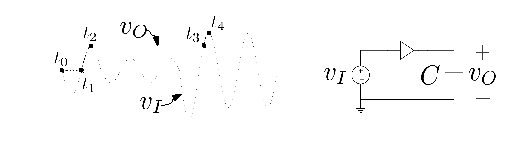
\includegraphics[scale=0.90]{peakDetector}
\caption{چوٹی حاصل کار}
\label{شکل_چوٹی_حاصل_کار}
\end{figure}
ڈایوڈ پر برقی دباو کے \عددی{\SI{0.7}{\volt}} گھٹنے کو نظر انداز کرتے ہوئے چوٹی حاصل کار کی کارکردگی کچھ یوں ہے۔وقت \عددی{t=0}\حاشیہد{\عددی{t_0} وغیرہ کو نقطوں سے ظاہر کیا گیا ہے} پر  \عددی{v_I} چالو کیا جاتا ہے۔لمحہ\عددی{t_0} یعنی \عددی{t=0} پر داخلی برقی دباو \عددی{v_I} اور خارجی برقی دباو \عددی{v_O} دونوں صفر وولٹ کے برابر ہیں۔لمحہ \عددی{t_0} سے لمحہ \عددی{t_1} تک داخلی برقی دباو ڈایوڈ کو الٹ مائل کرتے ہوئے منقطع رکھتا ہے اور یوں اس دوران \عددی{v_O} صفر رہے گا۔\عددی{t_1} سے \عددی{t_2} تک خارجی برقی دباو \عددی{v_O} خوش اسلوبی سے داخلی برقی دباو \عددی{v_I} کی پیروی کرتے ہوئے کپیسٹر کو چارج کرتا ہے۔اس دوران دور میں برقی رو کی مساوات مندرجہ ذیل ہے۔
\begin{align*}
i=C \frac{dv_O}{dt}
\end{align*}
\عددی{t_2} گزرتے ہی \عددی{v_I} کی قیمت کم ہونا شروع ہو جاتا ہے۔یوں \عددی{t_2} سے \عددی{t_3} تک \عددی{v_I< v_O} رہتا ہے جس کی وجہ سے ڈایوڈ منقطع رہتا ہے۔اس دوران کپیسٹر سے چارج کے نکاسی کا کوئی راستہ موجود نہیں ہوتا لہٰذا کپیسٹر پر برقی دباو برقرار رہتا ہے جسے افقی لکیر سے دکھایا گیا ہے۔\عددی{t_3} گزرتے ہی \عددی{v_I} کی قیمت کپیسٹر پر پائے جانے والے برقی دباو سے بڑھ گیا ہے۔یوں ڈایوڈ ایک بار پھر سیدھا مائل ہوتے ہوئے چالو صورت اختیار کر لیتا ہے۔\عددی{t_3} تا \عددی{t_4} \عددی{v_O} دوبارہ \عددی{v_I} کی پیروی کرتا ہے۔\عددی{t_4} کے بعد کپیسٹر پر برقی دباو تبدیل نہیں ہوتا۔

اس تجزیہ سے واضح ہے کہ یہ دور داخلی اشارہ کی چوٹی حاصل کر کے اس پر برقرار رہتا ہے۔اسی لئے اسے مثبت \موٹا{چوٹی حاصل کار}  کہتے ہیں۔اگر اس دور میں ڈایوڈ الٹے رخ لگایا جائے تو خارجی اشارہ \عددی{v_O}منفی چوٹی پر چارج ہو جائے گا اور یوں اس دور کو \موٹا{منفی چوٹی حاصل} کار کہا جائے گا۔

\حصہ{حیطہ اتار کار}
مثبت چوٹی حاصل کار میں کپیسٹر کے متوازی مزاحمت جوڑنے سے \موٹا{حیطہ اتار کار}\فرہنگ{حیطہ!اتار کار}\فرہنگ{AM demodulator}\حاشیہب{AM demodulator}  حاصل ہوتا ہے جسے شکل \حوالہ{شکل_حیطہ_اتر_کار}  میں دکھایا گیا ہے۔
\begin{figure}
\centering
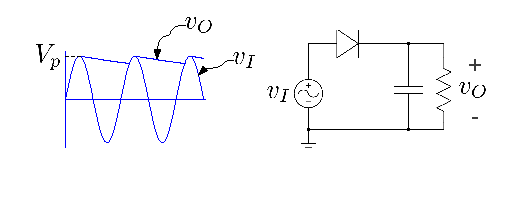
\includegraphics[scale=0.90]{demodulatorAM}
\caption{حیطہ اتار کار}
\label{شکل_حیطہ_اتر_کار}
\end{figure}
%
\begin{figure}
\centering
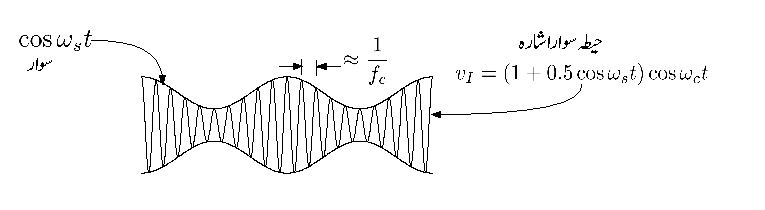
\includegraphics[scale=0.90]{AMmodulation}
\caption{حیطہ سوار اشارہ}
\label{شکل_حیطہ_سوار_اشارہ}
\end{figure}
جیسا کہ آپ دیکھ سکتے ہیں چوٹی \عددی{V_p} کے  فوراً بعد داخلی برقی دباو گھٹتا ہے جبکہ خارجی جانب کپیسٹر اسی چوٹی پر چارج رہ جاتا ہے۔اس سے ڈایوڈ الٹا مائل ہو جاتا ہے اور اس میں سے برقی رو کا گزر ناممکن ہو جاتا ہے۔ڈایوڈ کو منقطع تصور کریں تو ہمارے پاس چارج شدہ کپیسٹر \عددی{C}  اور اس کے متوازی جڑا مزاحمت \عددی{R} رہ جاتا ہے۔کپیسٹر کا چارج اسی مزاحمت کے راستے  خارج ہو کر اس پر برقی دباو گھٹاتا ہے۔ایسا مندرجہ ذیل مساوات کے تحت ہوتا ہے۔
\begin{align} \label{مساوات_حیطہ_اتار_کار_الف}
v_O=V_{p} e^{-\frac{t}{RC}}
\end{align}

اس مساوات میں چوٹی کو \عددی{t=0} تصور کیا گیا ہے۔کپیسٹر سے چارج اس لمحہ تک خارج ہوتا ہے جب تک کپیسٹر پر برقی دباو \عددی{v_O}  دور کے داخلی برقی دباو \عددی{v_I}  سے زیادہ رہے۔جیسے ہی \عددی{v_I}کی مقدار ایک بار پھر \عددی{v_O}کی مقدار سے تجاوز کر جائے، اسی لمحہ ڈایوڈ دوبارہ سیدھا مائل ہو کر کپیسٹر کو دوبارہ چارج کرنا شروع کر دیتا ہے۔شکل میں باریک لکیر سے داخلی برقی دباو جبکہ موٹی لکیر سے خارجی برقی دباو دکھایا گیا ہے۔\موٹا{حیطہ اتار کار} میں \عددی{RC} کو یوں رکھا جاتا ہے کہ  کپیسٹر پر \عددی{v_I} کے چوٹیوں کے برابر برقی دباو رہے جو دراصل \عددی{v_s} ہی ہے۔یوں اصل اشارہ دوبارہ حاصل ہوتا ہے۔

کسی بھی اشارہ یعنی اطلاع  \عددی{v_s} کو ایک جگہ سے دوسری جگہ منتقل کرنے کی خاطر اسے بلند تعدد کے سائن-نما اشارہ \عددی{v_c} کے حیطے پر \موٹا{حیطہ سوار کار}\فرہنگ{حیطہ!سوار کار}\فرہنگ{AM modulator}\حاشیہب{AM modulator} کی مدد سے سوار کیا جاتا ہے۔منتقلی کے مقام پر پہنچنے کے بعد \موٹا{حیطہ سوار اشارے} سے \موٹا{حیطہ اتار کار} کی مدد سے اصل اشارہ یعنی اطلاع کو \عددی{v_s} دوبارہ حاصل کیا جاتا ہے۔\عددی{v_c} کے حیطے پر سوار کرنے سے مراد \عددی{v_c} کے حیطے کو \عددی{v_s} کے مطابق تبدیل کرنے کو کہتے ہیں۔\عددی{v_s=0.5 \cos \omega_s t} کو مثال بناتے ہوئے آگے بڑھتے ہیں۔حیطہ سوار اشارہ حاصل کرنے کی خاطر \عددی{v_s} اور \عددی{v_c} کو \موٹا{حیطہ سوار کار} سے گزارا جاتا ہے جس سے 
\begin{align}\label{مساوات_ڈایوڈ_حیطہ_سوار_اشارہ}
v_I=\left(1+0.5 \cos \omega_s t \right) \cos \omega_c t=V_p \cos \omega t
\end{align}
حاصل ہوتا ہے۔اس اشارہ جس کو شکل \حوالہ{شکل_حیطہ_سوار_اشارہ} میں دکھایا گیا ہے کو \موٹا{حیطہ سوار اشارہ}\فرہنگ{حیطہ!سوار اشارہ}\حاشیہب{AM signal}\فرہنگ{AM signal} \عددی{v_I} کہتے ہیں۔

\عددی{v_I} کے دو متواتر چوٹیوں کے درمیان حیطہ اتار کار کے  کپیسٹر پر برقی دباو گھٹتا ہے۔یہ وقفہ تقریباً \عددی{\tfrac{1}{f_c}} کے برابر ہے جسے استعمال کرتے ہوئے  مساوات \حوالہ{مساوات_حیطہ_اتار_کار_الف} سے \موٹا{مسئلہ مکلارن} کی مدد سے وقفے کے آخر میں برقی دباو
\begin{align}
v_O=V_{p} e^{-\frac{1}{RC f_c}} \approx V_p \left(1-\frac{1}{RC f_c} +\cdots \right )
\end{align}
حاصل ہوتا ہے۔یوں اس دوران برقی دباو میں تبدیلی
\begin{align*}
\abs{\Delta v_O} =\frac{V_p}{RC f_c}
\end{align*}
حاصل ہوتی ہے یعنی اس وقفے کے دوران خارجی اشارے کی وقت کے ساتھ شرح تبدیلی 
\begin{align}\label{مساوات_ڈایوڈ_حیطہ_اتار_کار_خارجی_اشارہ}
\frac{\abs{\Delta v_O}}{\frac{1}{f_c}} =\frac{V_p}{RC}
\end{align}
ہے۔حیطہ اتار کار میں \عددی{RC} کو یوں رکھا جاتا ہے کہ  بھیجے گئے اشارے \عددی{v_s} میں زیادہ سے زیادہ تبدیلی کو بھی پکڑا جا سکے۔\عددی{v_s} میں تبدیلی کی شرح
\begin{align*}
\od{v_s}{t}=-0.5 \omega_s \sin \omega_s t
\end{align*}
ہے جس کی زیادہ سے زیادہ قیمت \عددی{\omega_s t=\tfrac{n \pi}{2}} پر حاصل ہوتی ہے جہاں \عددیء{n=1,3,5,\cdots} ہے۔یہ قیمت 
\begin{align*}
\abs{\od{v_s}{t}}=0.5 \omega_s 
\end{align*} 
ہے۔اس زیادہ سے زیادہ داخلی اشارے کے تبدیلی کی شرح کو \موٹا{حیطہ اتار کار} کے تبدیلی کے شرح کے برابر رکھا جاتا ہے۔\عددی{\omega_s t=\tfrac{n \pi}{2}} پر مساوات \حوالہ{مساوات_ڈایوڈ_حیطہ_سوار_اشارہ} کے تحت \عددی{V_p=1} حاصل ہوتا ہے جسے مساوات \حوالہ{مساوات_ڈایوڈ_حیطہ_اتار_کار_خارجی_اشارہ} میں استعمال کرتے ہوئے یوں
\begin{align}
\frac{1}{RC}=0.5 \omega_s
\end{align}
رکھا جاتا ہے۔یہ مساوات \موٹا{حیطہ اتار کار} کی مساوات ہے۔اگر کپیسٹر کو اس مساوات سے حاصل قیمت سے زیادہ رکھا جائے تب خارجی اشارہ تیزی سے تبدیل ہونے والے داخلی اشارے کو نہیں پکڑ سکے گا۔اگر کپیسٹر کی قیمت اس سے کم رکھی جائے تب خارجی اشارے میں \موٹا{بل}\فرہنگ{بل}\حاشیہب{ripple} زیادہ پایا جائے گا۔ 

\حصہ{پیدا کار برقی دباو}
سمت کار کے خارجی جانب زیادہ قیمت کا کپیسٹر نسب کر کے \موٹا{پیدا کار برقی دباو}\فرہنگ{پیدا کار برقی دباو}\فرہنگ{برقی دباو سپلائی}\حاشیہب{power supply}  حاصل ہوتا ہے جیسا شکل \حوالہ{شکل_پاور_سپلائی} الف میں دکھایا گیا ہے۔اس پر کپیسٹر کے متوازی برقی بار لادا جاتا ہے جسے عموماً \عددی{R_L} سے ظاہر کیا جاتا ہے۔\موٹا{پیدا کار برقی دباو} یعنی برقی طاقت کے \موٹا{سپلائی} کو  گھریلو بجلی یا صنعتی بجلی فراہم کرتے ہوئے یک سمتی برقی دباو \عددی{V_{\textrm{یکسمتی}}} حاصل کیا جاتا ہے۔
 
بے بار پیدا کار برقی دباو کی کارکردگی بالکل چوٹی حاصل کار کی طرح ہے جبکہ برقی بار سے لدے پیدا کار برقی دباو کی کارکردگی حیطہ اتار کار کی طرح ہے۔البتہ پیدا کار میں ہماری کوشش ہوتی ہے کہ  \عددی{V_{\textrm{یکسمتی}}} میں \موٹا{بل} کم سے کم ہو تا کہ اسے یک سمتی برقی دباو کے طور استعمال کرنا ممکن ہو۔پیدا کار برقی دباو تقریباً ہر برقیاتی آلہ یا مشین میں پایا جاتا ہے۔

چونکہ پیداکار برقی دباو داخلی طاقت \عددی{\SI{50}{\hertz}} کے سائن نما \عددی{v_i} سے حاصل کرتا ہے لہٰذا \عددی{C} بھی اسی تعدد سے چارج ہوتا ہے۔\عددی{v_i} کے دو چوٹیوں کے مابین \عددی{\tfrac{1}{50}=\SI{20}{\milli \second}}  (بیس ملی سیکنڈ )  کے وقفے  کے دوران \عددی{R_L} کو کپیسٹر \عددی{C} طاقت مہیا کرتا ہے۔
\begin{figure}
\centering
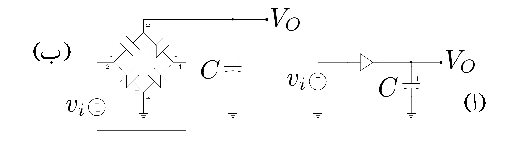
\includegraphics[scale=0.90]{powerSupply}
\caption{پیدا کار برقی دباو}
\label{شکل_پاور_سپلائی}
\end{figure}
\ابتدا{مثال} \شناخت{مثال_پیداکار_برقی_دباو}
ایک عدد \عددی{\SI{12}{\volt}} کا پیدا کار برقی دباو درکار ہے جس سے \عددی{\SI{6}{\kilo \ohm}} داخلی مزاحمت کے برقی بار کو طاقت مہیا کرنا ہے۔برقی بار کو دی جانے والے برقی دباو کے قیمت میں کل تبدیلی \عددی{\SI{\mp 0.5}{\volt}} سے کم ہونا ضروری ہے۔کپیسٹر \عددی{C} کی قیمت حاصل کریں۔

حل: 
شکل \حوالہ{شکل_مثال_پاور_سپلائی} میں ان معلومات کو دکھایا گیا ہے۔کپیسٹر \عددی{t_1} دورانیہ کے لئے  برقی بار کو طاقت فراہم کرتا ہے اور یوں اس دوران اس سے چارج کی نکاسی ہوتی ہے۔البتہ \عددی{t_1} کو دو چوٹیوں کے درمیان وقفے کے برابر ہی عموماً تصور کیا جاتا ہے۔یوں \عددی{t_1=\SI{20}{\milli \second}} لیا جاتا ہے۔

اس مسئلے کو دو طریقوں سے حل کرتے ہیں۔پہلے مثال \حوالہ{مثال_نصف_لہر_سمتکار_مستطیل_داخلی_دباو} کی طرح حل کرتے ہیں۔کپیسٹر نکاسی  کا دورانیہ بیس ملی سیکنڈ ہے۔اس دورانیہ میں  کپیسٹر پر  برقی دباو \عددی{\SI{12.5}{\volt}} سے گھٹ کر \عددی{\SI{11.5}{\volt}} رہ جاتا ہے یوں
\begin{align*}
11.5=12.5 e^{-\frac{0.02}{6000C}}\\
C=\SI{39.98}{\micro \farad}
\end{align*}
حاصل ہوتا ہے۔آئیں اسی مسئلے کو قدر مختلف اور زیادہ آسان طریقے سے حل کریں۔
% 
 \begin{figure}
\centering
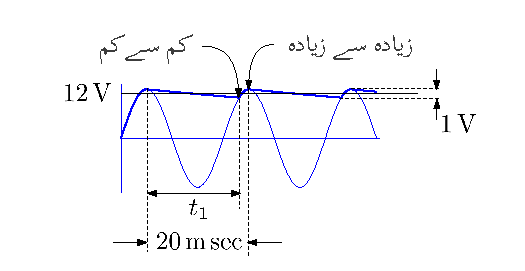
\includegraphics[scale=0.90]{powerSupplyA}
\caption{مثال پیدا کار برقی دباو}
\label{شکل_مثال_پاور_سپلائی}
\end{figure}

درکار بارہ وولٹ کو شکل \حوالہ{شکل_مثال_پاور_سپلائی} میں پختہ لکیر سے دکھایا گیا ہے۔برقی دباو اس سے \عددی{\SI{0.5}{\volt}} کم یا زیادہ ہو سکتا ہے۔یوں برقی بار میں \موٹا{بل}\فرہنگ{بل}\حاشیہب{ripple}\فرہنگ{ripple} \عددی{\SI{0.5}{\volt}} یا \عددی{\SI{1}{\volt}} کے برابر ہے جبکہ زیادہ سے زیادہ برقی دباو \عددی{\SI{12.5}{\volt}} اور کم سے کم برقی دباو \عددی{\SI{11.5}{\volt}} ہے۔بارہ وولٹ پر \عددی{R_L} میں \عددی{\tfrac{12}{6000}=\SI{2}{\milli \ampere}} جبکہ زیادہ سے زیادہ برقی دباو پر  \عددی{\tfrac{12.5}{6000}=\SI{2.08333}{\milli \ampere}} اور کم سے کم برقی دباو پر  \عددی{\tfrac{11.5}{6000}=\SI{1.9167}{\milli \ampere}} کا برقی رو گزرے گا۔

برقی دباو کے تبدیلی سے برقی رو کے تبدیلی کو نظر انداز کرتے ہوئے اس کی اوسط قیمت لی جاتی ہے۔یوں ہم تصور کرتے ہیں کہ \عددی{R_L} میں \عددی{\SI{2}{\milli \ampere}} گزرتا ہے جس سے کپیسٹر کے چارج کی نکاسی ہوتی ہے۔ہم جانتے ہیں کہ
\begin{align*}
I=\frac{\Delta Q}{\Delta t}
\end{align*}
کے برابر ہوتا ہے۔ اس سے کپیسٹر میں  \عددی{t_1} کے دوران کپیسٹر پر پائے جانے والے چارج میں تبدیلی \عددی{\Delta Q} حاصل کرتے ہیں۔
\begin{align*}
\Delta Q=I \times \Delta t=\left(2 \times 10^{-3} \right) \times \left(20 \times 10^{-3} \right)=40 \times 10^{-6}
\end{align*}
کپیسٹر کی مساوات \عددی{Q=CV} کو \عددی{\Delta Q=C \Delta V} لکھتے ہیں جہاں \عددی{\Delta V=\SI{1}{\volt}} کے برابر ہے۔یوں
\begin{align*}
\Delta Q=I \times \Delta t=C \Delta V
\end{align*}
لکھا جا سکتا ہے جس سے
\begin{align*}
C \times 1&=40 \times 10^{-6}\\
C&=\SI{40}{\micro \farad}
\end{align*}
حاصل ہوتا ہے۔

آپ نے دیکھا کہ دونوں طریقوں سے حل کرتے تقریباً برابر جوابات حاصل ہوتے ہیں۔البتہ دوسرا طریقہ استعمال کرتے ہوئے صرف کاغذ اور قلم استعمال کرتے ہوئے جواب کا حصول ممکن ہے۔
\انتہا{مثال}
%===============

کپیسٹر کی قیمت بڑھانے سے سپلائی کے خارجی برقی دباو میں \موٹا{بل} کم کیا جا سکتا ہے۔حقیقت میں ڈایوڈ میں برقی دباو کا گھٹاو اور داخلی بدلتے برقی دباو میں تبدیلی ہمارے قابو میں نہیں ہوتے لہٰذا اس طرح کے پیداکار برقی دباو سے قطعی یک سمتی برقی دباو کا حصول ممکن نہیں ہوتا۔جہاں درکار یک سمتی برقی دباو کی  قیمت چند وولٹ زیادہ یا کم  قابل برداشت ہو وہاں اس طرح کی سپلائی استعمال کی جا سکتی ہے۔یک سمتی برقی دباو کی قیمت زیادہ یا کم ہونے کے باوجود برقی دباو میں \موٹا{بل} کو کپیسٹر سے قابو رکھنا ممکن ہے۔


%================
\ابتدا{مشق}
\عددی{\SI{10}{\milli \ampere}} کے برقی بار کو چلانے کی خاطر \عددی{\SI{5}{\volt}} کا پیداکار برقی دباو درکار ہے جس میں \موٹا{بل} \عددی{\SI{\mp 0.1}{\volt}} سے کم ہونا ضروری ہے۔کپیسٹر کی قیمت حاصل کریں۔اس قسم کا \موٹا{پیداکار برقی دباو} برقیاتی ادوار کو چلانے کی خاطر عموماً درکار ہوتا ہے۔

جواب: \عددی{\SI{1000}{\micro \farad}}
\انتہا{مشق}
%================
مندرجہ بالا مثال کو مد نظر رکھتے ہوئے ہم دیکھتے ہیں کہ شکل \حوالہ{شکل_پاور_سپلائی} ب میں دکھائے پیدا کار برقی دباو میں درکار کپیسٹر کی قیمت شکل  الف کے حوالے سے آدھی ہو گی کیوں کہ اس میں ایک ڈایوڈ یعنی آدھے سمت کار کی جگہ مربع ڈایوڈ یعنی مکمل سمت کار استعمال کیا گیا ہے۔مکمل سمت کار میں کپیسٹر ہر \عددی{\SI{10}{\milli \second}} چارج ہو گا۔مثال \حوالہ{مثال_پیداکار_برقی_دباو} کو شکل \حوالہ{شکل_پاور_سپلائی} ب کے لئے حل کرتے ہوئے \عددی{t_1=\SI{10}{\milli \second}} لیا جائے گا جس سے \عددی{C=\SI{20}{\micro \farad}} حاصل ہوتا ہے۔ 
 
کامل ڈایوڈ تصور کرتے ہوئے خارجی برقی دباو کی زیادہ سے زیادہ قیمت \عددی{V_p} جبکہ اس میں کل \موٹا{بل} \عددی{\Delta V} لکھتے ہوئے
\begin{align}
V_{\textrm{یکسمتی}}=V_p-\frac{\Delta V}{2}
\end{align}
حاصل ہو گا۔
\جزوحصہ{برقیاتی شکنجہ}

عموماً برقیاتی اشارات مطلوبہ جگہ تک پہنچتے پہنچتے اپنی اصل شکل کھو جاتے ہیں۔ ایک عمومی مسئلہ اشارہ کے حیطہ کا برقرار نہ رہنا ہے۔آئیں اس کی ایک مثال دیکھیں۔

آپ جانتے ہیں کہ بدلتی برقی رو مقناطیس پیدا کرتی ہے اور بدلتی مقناطیسی میدان برقی دباو کو جنم دیتا ہے۔یوں اگر باریک اشاراتی تاروں کے قریب عام استعمال کے گھریلو یا صنعتی بجلی کے تار گزریں تو ان میں بدلتی برقی رو باریک اشاراتی تاروں میں برقی دباو پیدا کرتا ہے جس سے اشارہ کا حیطہ متاثر ہوتا ہے۔شکل \حوالہ{شکل_شکنجہ}  میں اشارہ \عددی{v_I}  کا حیطہ یوں متاثر ہوا دکھایا گیا ہے۔یہ اشارہ دراصل سائن شکل کا تھا لیکن یہاں تک پہنچتے پہنچتے اس کا یہ حال ہو چکا ہے۔شکل \حوالہ{شکل_شکنجہ}  میں دکھایا دور اشارہ کے مثبت حیطہ کو \عددی{V_r} کی قیمت پر زبردستی رکھتا ہے جس سے اشارہ کی اصل صورت رو نما ہو جاتی ہے۔ گویا یہ دور اشارہ کے حیطہ کو شکنجہ میں پکڑے رکھتا ہے۔اسی سے اس دور کا نام \موٹا{برقیاتی شکنجہ}\فرہنگ{شکنجہ}\فرہنگ{clamping circuit}\حاشیہب{clamping circuit}  نکلا ہے جسے عموماً چھوٹا  کر کے صرف \موٹا{شکنجہ} کہتے ہیں
\begin{figure}
\centering
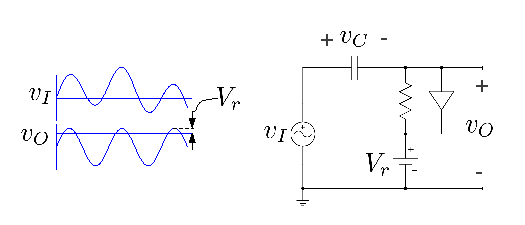
\includegraphics[scale=0.90]{clampingCircuit}
\caption{شکنجہ}
\label{شکل_شکنجہ}
\end{figure}
اس دور کی کارکردگی پچھلے حصہ میں دکھلائے دور کی طرح ہے۔اسے سمجھنے کی خاطر ڈایوڈ   کو کامل ڈایوڈ اور مزاحمت \عددی{R} کو لامحدود تصور کریں۔یہ بھی تصور کریں کہ داخلی اشارہ \عددی{v_I} کے حیطہ \عددی{v_p} کی مقدار خارجی جانب جڑے بیٹری کی برقی دباو \عددی{V_r} سے زیادہ ہے۔


خارجی جانب کی برقی دباو \عددی{v_O} پر غور کرتے معلوم ہوتا ہے کہ یہ کسی صورت \عددی{V_r} سے تجاوز نہیں کر سکتا کیوں کہ جب بھی \عددی{v_O} کی مقدار \عددی{V_r} سے تجاوز کرے،  ڈایوڈ سیدھا مائل ہو جائے گا۔سیدھے مائل ڈایوڈ کی صورت میں \عددی{v_O} اور \عددی{V_r} برابر رہیں گے۔کرچاف کے قانون برائے برقی دباو کے تحت سیدھے مائل ڈایوڈ کی صورت میں
\begin{align*}
v_I=v_C+v_D+V_r
\end{align*}
ہو گا۔داخلی برقی دباو کے چوٹی پر \عددی{v_D} کو صفر وولٹ اور \عددی{v_I} کو \عددی{v_p} لیتے ہوئے اس مساوات سے کپیسٹر کا برقی دباو یوں حاصل ہوتا ہے
\begin{align*}
v_C= v_I-v_D-V_r \approx v_p - V_r
\end{align*}
یوں کپیسٹر اس برقی دباو پر رہتے ہوئے خارجی برقی دباو کے مثبت حیطہ کو \عددی{V_r} سے تجاوز کرنے سے روکتا ہے۔

جیسا کہ پہلے ذکر ہوا اصل استعمال میں داخلی اشارہ کا حیطہ از خود کم اور زیادہ ہوتا ہے۔اس صورت کو شکل میں دکھایا گیا ہے۔اس صورت سے نمٹنے کی خاطر دور میں ڈایوڈ کے متوازی مزاحمت \عددی{R} نسب کی گئی ہے تا کہ اس کے راستے کپیسٹر کا چارج خارج ہو سکے اور یہ بعد میں آنے والی کم چوٹی کو بھی قابو کر سکے۔


\حصہ{برقیاتی تراش}

شکنجہ کے دور میں کپیسٹر کی جگہ مزاحمت استعمال کرنے سے \موٹا{برقیاتی تراش}\فرہنگ{تراش}\فرہنگ{clipper}\حاشیہب{clipper}  کا دور حاصل ہوتا ہے جسے شکل \حوالہ{شکل_ایک_طرف_کا_تراش} میں دکھایا گیا ہے۔\موٹا{برقیاتی تراش} یا \موٹا{تراش} ایک ایسا دور ہے جو اشارہ کے چوٹی کو ایک خاص حد سے تجاوز نہیں کرنے دیتا بلکہ اسے کاٹ دیتا ہے۔دکھایا دور صرف ایک جانب کی چوٹی کاٹتا ہے لہٰذا اس کو \موٹا{ایک طرف کا تراش} کہا جائے گا۔
 \begin{figure}
\centering
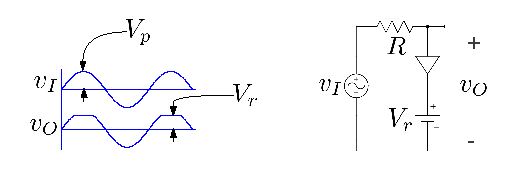
\includegraphics[scale=0.90]{clipperOneSided}
\caption{ایک طرف کا تراش}
\label{شکل_ایک_طرف_کا_تراش}
\end{figure}
جب تک داخلی برقی دباو کی قیمت \عددی{V_r} سے کم ہو ڈایوڈ الٹ مائل یعنی منقطع رہتا ہے۔اس صورت میں خارجی برقی دباو داخلی برقی دباو کے برابر رہے گا یعنی ہو گا اور مزاحمت \عددی{R}  میں برقی رو کی مقدار صفر ایمپیئر رہے گی۔جیسے ہی داخلی برقی دباو  کی قیمت \عددی{V_r} سے تجاوز کر جائے ڈایوڈ سیدھا مائل ہو جاتا ہے۔ جتنی دیر  \عددی{v_I>V_r} رہے اتنی دیر کے لئے  ڈایوڈ کو چالو سوئچ سمجھا جا سکتا ہے اور یوں اس دوران خارجی برقی دباو کی قیمت \عددی{V_r} رہے گی۔اس دوران مزاحمت اور ڈایوڈ دونوں میں برقی رو کی مقدار
\begin{align*}
i_R=\frac{v_I-V_r}{R}
\end{align*}
ہو گی۔

آپ نے دیکھا کہ یہ دور داخلی برقی دباو کو \عددی{V_r} پر تراشتا ہے۔اس دور میں دو ڈایوڈ کے استعمال سے دو اطراف کا تراش حاصل ہوتا ہے جسے شکل \حوالہ{شکل_دو_اطراف_کا_تراش}  میں دکھایا گیا ہے۔
\begin{figure}
\centering
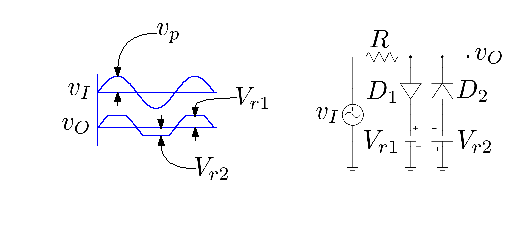
\includegraphics[scale=0.90]{clipperDoubleSided}
\caption{دو اطراف کا تراش}
\label{شکل_دو_اطراف_کا_تراش}
\end{figure}
اس دور میں جب تک \عددی{v_I} کی قیمت مثبت ہو ڈایوڈ \عددی{D_2} الٹا مائل رہتا ہے۔یوں مثبت داخلی برقی دباو کے لئے یہ دور بالکل پچھلے دئے گئے ایک طرف کے تراش کی طرح کام کرتا ہے اور داخلی اشارہ کے مثبت چوٹی کو \عددی{V_{r1}} پر تراشتا ہے۔

منفی داخلی برقی دباو کی صورت میں ڈایوڈ \عددی{D_1} الٹ مائل رہتا ہے اور یہ دور داخلی اشارہ کے منفی چوٹی کو \عددی{V_{r2}} پر تراشتا ہے۔شکل میں داخلی اور تراشے گئے خارجی برقی دباو بھی دکھائے گئے ہیں۔

\حصہ{حسابی ایمپلیفائر کی مدد سے ڈایوڈ کے کامل ادوار}
\جزوحصہ{کامل نصف لہر سمت کار}
ڈایوڈ پر مبنی \موٹا{نصف لہر سمت کار} کے خارجی اشارے کی چوٹی مہیا کردہ داخلی اشارے کے چوٹی سے تقریباً \عددی{\SI{0.7}{\volt}} کم ہوتی ہے۔یہ حقیقت شکل \حوالہ{شکل_نصف_لہر_مثبت_سمت_کار} میں واضح کی گئی۔حسابی ایمپلیفائر استعمال کرتے ہوئے ایسا کامل نصف لہر سمت کار حاصل ہوتا ہے  جس کے خارجی اشارے کی چوٹی داخلی اشارے کے چوٹی کے بالکل برابر ہوتی ہے۔شکل\حوالہ{شکل_کامل_نصف_لہر_سمت_کار} الف میں ایسا کامل نصف لہر مثبت سمت کار دکھایا گیا ہے جس میں خارجی اشارہ \عددی{v_o} کو ڈایوڈ کے خارجی سرے سے حاصل کیا گیا ہے۔ڈایوڈ کی سمت الٹانے سے  کامل نصف لہر منفی سمت کار حاصل ہو گا۔
\begin{figure}
\centering
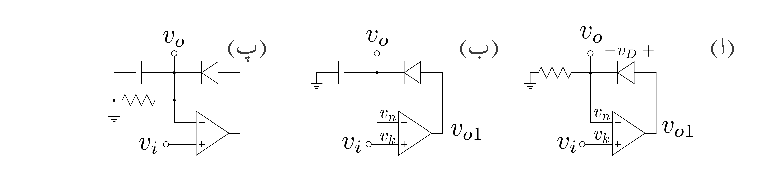
\includegraphics[scale=0.90]{opampHalfWaveRectifierPeakDetector}
\caption{کامل ادوار}
\label{شکل_کامل_نصف_لہر_سمت_کار}
\end{figure}

تصور کریں کہ \عددی{v_i=\SI{0}{\volt}} اور یوں حسابی ایمپلیفائر کا خارجی اشارہ \عددی{v_{o1}} بھی صفر وولٹ ہے۔اب تصور کریں کہ داخلی اشارہ مثبت جانب بڑھتا ہے۔حسابی ایمپلیفائر کا خارجی اشارہ اس قدر مثبت جانب بڑھے گا کہ \عددی{v_k=v_n} یعنی \عددی{v_k=v_i} ہو۔یوں \عددی{v_o=v_i} ہو گا۔آپ دیکھ سکتے ہیں کہ اس صورت میں ڈایوڈ سیدھا مائل ہو گا۔مزید یہ کہ \عددی{v_{o1}=v_i+v_D} کے برابر ہو گا۔

اب تصور کریں کہ داخلی اشارہ منفی جانب بڑھتا ہے۔حسابی ایمپلیفائر کا خارجی اشارہ \عددی{v_{o1}} اس قدر منفی جانب بڑھنے کی کوشش کرے گا کہ \عددی{v_k=v_n} ہوں۔البتہ \عددی{v_{o1}} منفی ہوتے ہی ڈایوڈ الٹا مائل ہو کر منقطع ہو جاتا ہے۔یوں حسابی ایمپلیفائر کا خارجی اشارہ \عددی{v_k} پر اثر انداز نہیں ہو پاتا۔ایسی صورت میں حسابی ایمپلیفائر کا خارجی اشارہ مکمل منفی یعنی \عددی{v_{o1}=V_{EE}} ہو کر رہ جائے گا۔ڈایوڈ منقطع ہونے سے  حسابی ایمپلیفائر کا منفی مداخل مزاحمت \عددی{R} کے ذریعہ برقی زمین سے جڑ جاتا ہے۔حسابی ایمپلیفائر کا داخلی برقی رو صفر ہونے کے ناطے مزاحمت میں بھی برقی رو \عددی{I} کا گزر ممکن نہیں۔یوں \عددی{v_k=I R=0} یعنی \عددی{v_o=\SI{0}{\volt}} ہو گا۔آپ دیکھ سکتے ہیں کہ منفی داخلی اشارے کی صورت میں خارجی اشارہ صفر وولٹ رہتا ہے۔

مثبت داخلی اشارے کی صورت میں \عددی{v_o=v_i} جبکہ منفی داخلی اشارے کی صورت میں \عددی{v_o=\SI{0}{\volt}} حاصل ہوتا ہے جو کہ مثبت نصف لہر سمت کار کی کارکردگی ہے۔

\جزوحصہ{کامل چوٹی حاصل کار}
شکل \حوالہ{شکل_کامل_نصف_لہر_سمت_کار} الف میں مزاحمت کی جگہ کپیسٹر نسب کرنے سے شکل  ب حاصل ہوتا ہے جو کامل مثبت \موٹا{چوٹی حاصل کار} کا دور ہے۔\عددی{v_i=\SI{0}{\volt}} اور \عددی{v_o=\SI{0}{\volt}} سے شروع کرتے ہوئے اس دور کی کارکردگی دیکھتے ہیں۔داخلی اشارہ مثبت جانب بڑھنے سے \عددی{v_{o1}} اس قدر بڑھتا ہے کہ \عددی{v_k=v_n} رہے۔یوں \عددی{v_o=v_i} رہتا ہے۔جب داخلی اشارہ اپنے چوٹی \عددی{V_p} پر پہنچتا ہے، اس لمحہ \عددی{v_k=V_p} اور یوں \عددی{v_n=V_p} ہوتا ہے۔ اس لمحہ کپیسٹر بھی \عددی{V_p} برقی دباو پر چارج ہو جاتا ہے۔\عددی{v_k=v_n} حاصل کرنے کی خاطر اس لمحہ \عددی{v_{o1}=V_P+v_D} کے برابر ہو گا۔

داخلی اشارہ اپنے چوٹی تک پہنچنے کے بعد کم ہونا شروع ہوتا ہے۔حسابی ایمپلیفائر کا خارجی اشارہ \عددی{v_{o1}} کم ہو کر کوشش کرتا ہے کہ \عددی{v_k=v_n} رکھ سکے۔البتہ ڈایوڈ کے خارجی جانب نسب کپیسٹر پر \عددی{V_p} برقی دباو پایا جاتا ہے اور \عددی{v_{o1}} کی قیمت جیسے ہی \عددی{V_p} سے کم ہوتا ہے اسی لمحہ ڈایوڈ الٹ مائل ہو کر منقطع ہو جاتا ہے۔ڈایوڈ منقطع ہونے سے کپیسٹر پر چارج کے نکاسی  کا کوئی راستہ نہیں رہتا اور یوں اس پر برقرار \عددی{V_p} برقی دباو رہتا ہے۔اس طرح \عددی{v_o=V_p} رہتا ہے۔ 

آپ نے دیکھا کہ کپیسٹر پر داخلی اشارے کے چوٹی کے بالکل برابر برقی دباو حاصل ہوتا ہے جسے بطور خارجی اشارہ \عددی{v_o} لیا جاتا ہے۔صرف ڈایوڈ پر مبنی چوٹی حاصل کار میں کپیسٹر پر داخلی اشارے کے چوٹی سے \عددی{v_D} برابر کم برقی دباو پایا جاتا ہے جبکہ موجودہ دور حقیقی چوٹی حاصل کرتا ہے۔

\جزوحصہ{کامل حیطہ اتار کار}
شکل \حوالہ{شکل_کامل_نصف_لہر_سمت_کار} پ میں کامل \موٹا{حیطہ اتار کار} دکھایا گیا ہے۔امید کی جاتی ہے کہ اس کی کارکردگی  آپ خود سمجھ پائیں گے۔

\جزوحصہ{ڈایوڈ لاگ ایمپلیفائر}
حسابی منفی ایمپلیفائر میں مزاحمت کی جگہ ڈایوڈ نسب کرنے سے شکل \حوالہ{شکل_ڈایوڈ_لاگ_ایمپلیفائر} الف کا \موٹا{لاگ ایمپلیفائر}\فرہنگ{لاگ ایمپلیفائر}\فرہنگ{log amplifier}\حاشیہب{log amplifier} حاصل ہوتا ہے۔مثبت \عددی{v_i} کی صورت میں \عددی{v_o} منفی ہو گا جس سے \عددی{D_1} سیدھا مائل جبکہ \عددی{D_2} الٹا مائل ہو گا۔اسی طرح منفی  \عددی{v_i} کی صورت میں \عددی{v_o} مثبت ہو گا جس سے \عددی{D_1} الٹا مائل جبکہ \عددی{D_2} سیدھا مائل ہو گا۔یوں کسی بھی وقت ایک ڈایوڈ منقطع رہتا ہے جبکہ دوسرا سیدھا مائل رہتا ہے۔اگرچہ حقیقت میں منفی متغیرہ کا لاگ نہیں پایا جاتا اور یوں دور میں صرف \عددی{D_1} ہونا چاہئے تھا لیکن عموماً دو ڈایوڈ استعمال کئے جاتے ہیں۔یوں داخلی اشارہ  مثبت یا منفی ممکن ہوتا ہے۔

مثبت \عددی{v_i} کی صورت میں حل کرتے ہیں۔حسابی ایمپلیفائر کے مثبت مداخل برقی زمین کے ساتھ جڑا ہے لہٰذا اس پر برقی دباو \عددی{v_k} صفر ہو گا۔منفی مداخل پر برقی دباو \عددی{v_n} لکھتے ہوئے کرچاف کے قانون برائے برقی رو کی مدد سے
\begin{align*}
\frac{v_n-v_i}{R}+i_D=0
\end{align*}
لکھا جا سکتا ہے جہاں \عددی{i_D} ڈایوڈ \عددی{D_1} کی برقی رو ہے۔اس مساوات میں  \عددی{v_n=0} اور \عددی{i_D} کی جگہ ڈایوڈ کی مساوات استعمال کرتے ہوئے 
\begin{align*}
\frac{v_n-v_i}{R}+I_S e^{\frac{v_n-v_o}{V_T}}=0\\
-\frac{v_i}{R}+I_S e^{\frac{-v_o}{V_T}}=0\\
\frac{v_i}{I_S R}= e^{\frac{-v_o}{V_T}}
\end{align*}
حاصل ہوتا ہے جہاں ڈایوڈ پر برقی دباو کو \عددی{v_n-v_o} لیا گیا ہے۔دونوں جانب \موٹا{قدرتی لاگ}\حاشیہب{natural log} لیتے ہوئے حاصل ہوتا ہے۔
\begin{align*}
v_o=-V_T \ln {\left( \frac{v_i}{I_S R} \right)}
\end{align*}
%
\begin{figure}
\centering
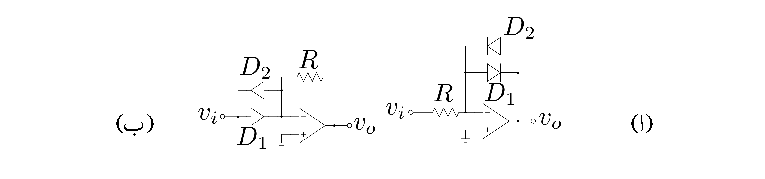
\includegraphics[scale=0.90]{logAmplifier}
\caption{لاگ ایمپلیفائر}
\label{شکل_ڈایوڈ_لاگ_ایمپلیفائر}
\end{figure}

شکل  ب میں  \موٹا{قدرتی الٹ-لاگ ایمپلیفائر}\فرہنگ{الٹ لاگ}\فرہنگ{anti-log}\حاشیہب{natural anti-log} دکھایا گیا ہے۔حسابی ایمپلیفائر کے دونوں مداخل کو برقی زمین تصور کرتے ہوئے مثبت \عددی{v_i} کی صورت میں ڈایوڈ \عددی{D_1} سیدھا مائل ہوتے ہوئے
\begin{align*}
i_D&=I_S e^{\frac{v_i-v_n}{V_T}}\\
&=I_S e^{\frac{v_i}{V_T}}
\end{align*}
برقی رو گزارے گا جو حسابی ایمپلیفائر کے منفی مداخل پر مزاحمت کی جانب مڑ جائے گا۔یوں
\begin{align*}
I_S e^{\frac{v_i}{V_T}}=\frac{v_n-v_o}{R}\\
v_o=-I_S R e^{\frac{v_i}{V_T}}
\end{align*}
حاصل ہوتا ہے۔آپ دیکھ سکتے ہیں کہ یہ دور داخلی اشارے کا \موٹا{قدرتی الٹ-لاگ} حاصل کرتا ہے۔
%===================
\جزوحصہ{ضرب کار}
\عددی{v_A} اور \عددی{v_B} کے لاگ جمع کرنے سے \عددی{\ln v_A+\ln v_B=\ln v_A v_B} حاصل ہوتا ہے جس کا الٹ-لاگ لینے سے \عددی{v_A v_B} یعنی دونوں متغیرات کا حاصل ضرب حاصل ہوتا ہے۔اسی حقیقت کو استعمال کرتے ہوئے لاگ اور الٹ-لاگ ایمپلیفائر استعمال کرتے  ہوئے شکل \حوالہ{شکل_ڈایوڈ_ضرب_کار} میں \موٹا{ضرب کار}\فرہنگ{ضرب کار}\حاشیہب{multiplier}\فرہنگ{multiplier} حاصل کیا گیا ہے۔لاگ ایمپلیفائر کے مساوات استعمال کرتے ہوئے ہم لکھ سکتے ہیں۔

\begin{align*}
v_{o1}&=-V_T \ln \frac{v_{i1}}{I_S R}\\
v_{o2}&=-V_T \ln \frac{v_{i1}}{I_S R}
\end{align*}
اسی طرح جمع کار کے مساوات سے 
\begin{align*}
v_{o3}&=-\left(v_{o1}+v_{o2} \right)\\
&=V_T \ln \frac{v_{i1}}{I_S R}+V_T \ln \frac{v_{i2}}{I_S R}\\
&=V_T \ln \frac{v_{i1} v_{i2}}{I_S^2 R^2}
\end{align*}
اور الٹ-لاگ کے مساوات سے
\begin{align*}
v_0&=-I_S R e^{\frac{v_{o3}}{V_T}}\\
&=-I_S R e^{\ln \frac{v_{i1} v_{i2}}{I_S^2 R^2}}\\
&=-\frac{v_{i1} v_{i2}}{I_S R}
\end{align*}
حاصل ہوتا ہے۔یہ \موٹا{ضرب کار} داخلی متغیرات کو آپس میں ضرب دیتے ہوئے \عددی{\frac{-1}{I_S  R}} سے بھی ضرب دیتا ہے۔

شکل میں جمع کار کی بجائے منفی کار کے استعمال سے \موٹا{تقسیم کار}\فرہنگ{تقسیم کار}\حاشیہب{divider}\فرہنگ{divider} حاصل ہوتا ہے۔
%
\begin{figure}
\centering
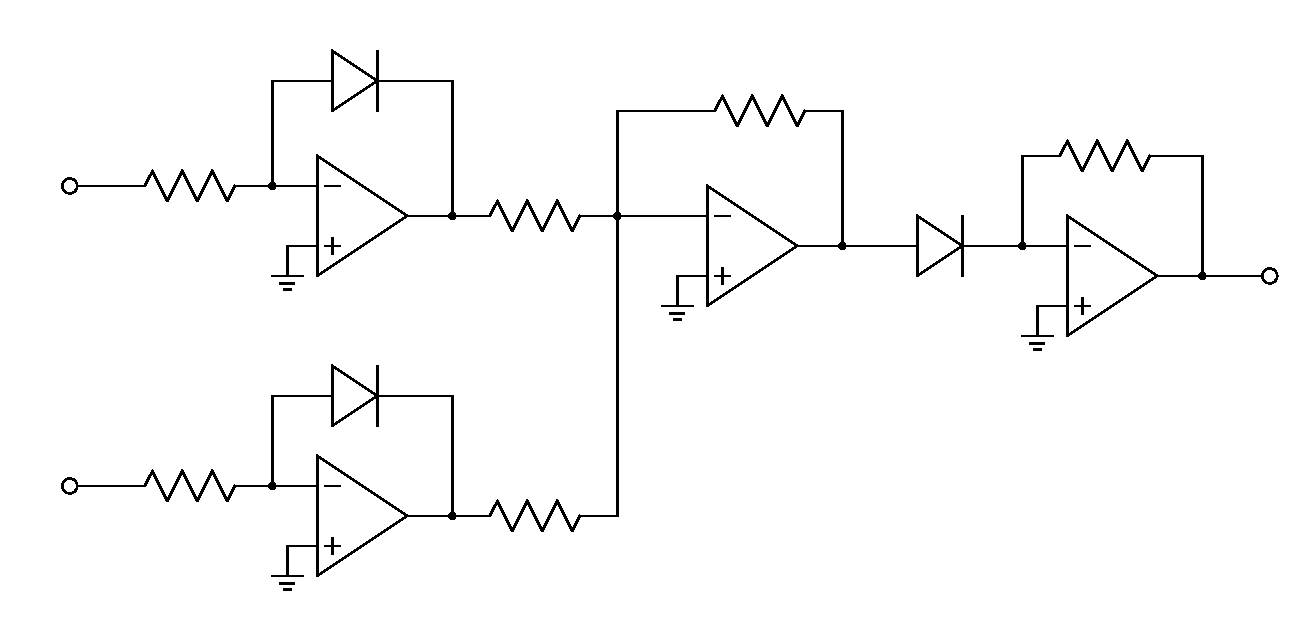
\includegraphics[scale=0.90]{multiplierDiode}
\caption{ضرب کار}
\label{شکل_ڈایوڈ_ضرب_کار}
\end{figure}



%==================

\جزوحصہ{کامل مکمل لہر سمت کار}
شکل \حوالہ{شکل_کامل_مکمل_لہر_سمت_کار} میں کامل \موٹا{مکمل لہر سمت کار} دکھایا گیا ہے۔آئیں اس کی کارکردگی مثبت اور منفی \عددی{v_i} کی صورت میں دیکھیں۔

مثبت \عددی{v_i} کی صورت میں \عددی{v_{o1}} منفی ہو جائے گا جس سے \عددی{D_1} الٹا مائل ہو کر منقطع جبکہ \عددی{D_2} سیدھا مائل ہو جائے گا۔\عددی{D_2} سیدھا مائل ہونے سے  \عددی{U_1} پر \عددی{v_n=v_k}  ہو گا۔\عددی{D_1} کو منقطع اور \عددی{U_1} کے منفی مداخل کو برقی زمین پر تصور کرتے ہوئے  شکل \حوالہ{شکل_کامل_مکمل_لہر_سمت_کار_الف} الف حاصل ہوتا ہے جو کہ سیدھا سادہ جمع کار ہے جس سے
\begin{align*}
v_o=-v_i
\end{align*}
حاصل ہوتا ہے۔ شکل \حوالہ{شکل_کامل_مکمل_لہر_سمت_کار_الف} الف میں \عددی{v_1} بھی دکھایا گیا ہے۔چونکہ اس کے دونوں جانب مزاحمتوں کے سرے صفر وولٹ پر ہیں لہٰذا اس صورت \عددی{v_1=\SI{0}{\volt}} رہے گا۔شکل \حوالہ{شکل_کامل_مکمل_لہر_سمت_کار_الف} ت میں مثبت \عددی{v_i} کی صورت میں \عددی{v_o} اور \عددی{v_1} دکھائے گئے ہیں۔
\begin{figure}
\centering
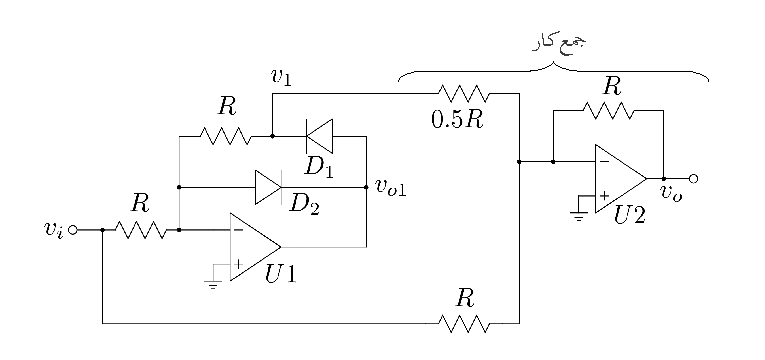
\includegraphics[scale=0.90]{opampFullWaveRectifier}
\caption{کامل مکمل لہر سمت کار}
\label{شکل_کامل_مکمل_لہر_سمت_کار}
\end{figure}
%
\begin{figure}
\centering
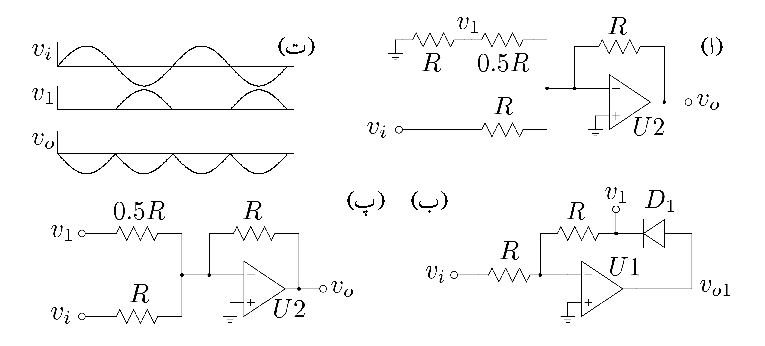
\includegraphics[scale=0.90]{opampFullWaveRectifierA}
\caption{کامل مکمل لہر سمت کار کی کارکردگی}
\label{شکل_کامل_مکمل_لہر_سمت_کار_الف}
\end{figure}

منفی \عددی{v_i} کی صورت میں \عددی{v_{o1}} مثبت ہو جائے گا جس سے \عددی{D_2} الٹا مائل ہو کر منقطع جبکہ \عددی{D_1} سیدھا مائل ہو جائے گا۔یوں \عددی{U_1} حسابی ایمپلیفائر شکل \حوالہ{شکل_کامل_مکمل_لہر_سمت_کار_الف} ب صورت اختیار کر لے گا جس کے لئے ہم لکھ سکتے ہیں
\begin{align*}
v_k=0\\
\frac{v_n-v_i}{R}+\frac{v_k-v_1}{R}=0
\end{align*}
اور یوں
\begin{align*}
v_1=-v_i
\end{align*}
حاصل ہوتا ہے۔آپ دیکھ سکتے ہیں کہ \عددی{v_{o1}=v_1+v_D} ہو گا جہاں \عددی{v_D} سیدھے مائل ڈایوڈ \عددی{D_1} پر برقی دباو ہے۔ \عددی{v_1} کے استعمال سے جمع کار کو شکل \حوالہ{شکل_کامل_مکمل_لہر_سمت_کار_الف} پ کے طرز پر بنایا جا سکتا ہے جس سے
\begin{align*}
v_o=-v_i-2 v_1
\end{align*}
حاصل ہوتا ہے۔شکل \حوالہ{شکل_کامل_مکمل_لہر_سمت_کار_الف} ت میں منفی \عددی{v_i} کی صورت میں \عددی{v_1} اور \عددی{v_o} دکھائے گئے ہیں۔

\حصہ{ڈایوڈ کے منتقی ادوار}
 ڈایوڈ پر مبنی ادوار حل کرنے کے طریقہ پر اس حصہ میں غور کیا جائے گا۔ ڈایوڈ پر مبنی ادوار حل کرتے وقت اگر سیدھے مائل اور اُلٹے مائل ڈایوڈوں  کہ نشاندہی کر دی جائے تو ان ادوار کو حل کرنا نہایت آسان ہو جاتا ہے۔اس صورت میں سیدھے مائل ڈایوڈوں کی جگہ چالو سوئچ اور اُلٹے مائل ڈایوڈوں  کی جگہ منقطع سوئچ نسب کر کے دور کو حل کیا جا سکتا ہے۔بدقسمتی سے قبل از وقت یہ جاننا کہ کون کون سے ڈایوڈ سیدھے مائل اور کون کون سے ڈایوڈ  اُلٹے مائل ہیں عموماً ناممکن ہوتا ہے۔ ڈایوڈ کے ادوار حل کرنے کا کوئی ایک سادہ طریقہ نہیں پایا جاتا البتہ گھبرانے کی بات نہیں چونکہ ایسے ادوار حل کرنے کے مشق سے یہ اندازہ لگانا کہ کون کون سے ڈایوڈ سیدھے یا الٹے مائل ہیں عموماً ممکن ہوتا ہے۔اس طریقہ کو مشق سے بہتر سیکھا جا سکتا ہے۔ایسا کرنے کی خاطر شکل \حوالہ{شکل_منتقی_جمع} میں دئے دور پر غور کریں۔
\begin{figure}
\centering
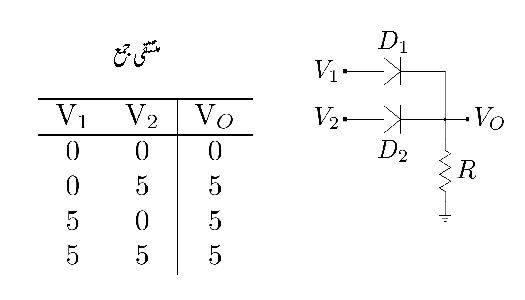
\includegraphics[scale=0.90]{diodeORgate}
\caption{منتقی جمع}
\label{شکل_منتقی_جمع}
\end{figure}

اس دور میں دو ڈایوڈ استعمال کئے گئے ہیں۔دور کے دو غیر تابع داخلی برقی دباو (اشارات) کو \عددی{V_1} اور \عددی{V_2} جبکہ خارجی برقی دباو کو \عددی{V_O} کہا گیا ہے۔ یہ ایک مخصوص دور ہے جس کے داخلی برقی دباو کے دو ہی ممکنہ قیمتیں ہیں۔ یہ تو یا صفر وولٹ \عددی{(\SI{0}{\volt})}   اور یا پھر پانچ وولٹ \عددی{(\SI{5}{\volt})}  ہو سکتے ہیں۔یوں داخلی جانب چار ممکنہ صورتیں پائی جاتی ہیں جنہیں شکل میں بطور جدول  دکھایا گیا ہے۔آئیں باری باری ان چار صورتوں پر غور کریں۔

پہلی صورت میں دونوں داخلی برقی دباو صفر وولٹ ہیں یعنی \عددی{V_1=0} اور \عددی{V_2=0} ہیں۔یہ جدول کی پہلی صف میں دکھایا گیا ہے۔اس صورت میں واضح ہے کہ دور میں برقی رو ممکن نہیں۔یوں خارجی جانب نسب مزاحمت میں برقی رو صفر ہونے کی وجہ سے اس کے سروں کے مابین برقی دباو بھی صفر وولٹ ہو گا۔جدول کی پہلی صف میں دائیں جانب \عددی{V_O} کی صف میں \عددی{0} اسی کو ظاہر کرتا ہے۔

دوسری صورت  \عددی{V_1} صفر وولٹ جبکہ \عددی{V_2}  پانچ وولٹ کے برابر ہے یعنی \عددی{V_1=\SI{0}{\volt}} جبکہ \عددی{V_2=\SI{5}{\volt}} ہے۔اس صورت کو جدول کے دوسری صف میں دکھایا گیا ہے۔غور کرنے سے آپ دیکھ سکتے ہیں کہ اس صورت میں ڈایوڈ \عددی{D_2} سیدھا مائل جبکہ \عددی{D_1} الٹ مائل ہے۔یوں \عددی{D_2}  کو چالو سوئچ جبکہ \عددی{D_1} کو منقطع سوئچ تصور کر کے یہ واضح ہے کہ خارجی برقی دباو پانچ وولٹ ہے یعنی \عددی{V_O=\SI{5}{\volt}}  ہے۔

	اسی طرح جدول کی تیسری صف کے حوالے سے \عددی{D_1} سیدھا مائل جبکہ \عددی{D_2} الٹ مائل ہو گا اور یوں \عددی{V_O=5} ہو گا۔جدول کی آخری صف  میں دونوں ڈایوڈ سیدھے مائل ہوں گے اور یوں \عددی{V_O=5} ہو گا۔
	اس دور کی جدول منتقی جمع کو ظاہر کرتی ہے لہٰذا یہ  \موٹا{جمع گیٹ}\فرہنگ{گیٹ!جمع}\فرہنگ{gate!OR}\حاشیہب{OR gate}  ہے۔اس شکل میں مزید  ڈایوڈ جوڑ کر داخلی اشارات کی تعداد بڑھائی جا سکتی ہے۔ 


\begin{figure}
\centering
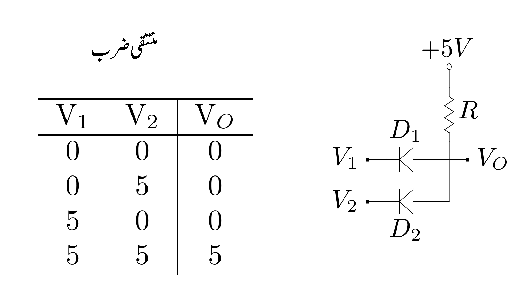
\includegraphics[scale=0.90]{diodeANDgate}
\caption{منتقی ضرب}
\label{شکل_منتقی_ضرب}
\end{figure}
شکل \حوالہ{شکل_منتقی_ضرب} میں ڈایوڈ   پر مبنی \موٹا{ضرب گیٹ}\فرہنگ{گیٹ!ضرب}\فرہنگ{gate!AND}\حاشیہب{AND gate}  دکھایا گیا ہے۔پہلے جدول میں دئے آخری صف پر غور کرتے ہیں۔اگر دونوں داخلی اشارات کی قیمتیں پانچ وولٹ \عددی{(\SI{5}{\volt})} ہوں تو مزاحمت میں برقی رو صفر ایمپیئر ہو گی لہٰذا خارجی برقی دباو بھی پانچ وولٹ ہو گا یعنی \عددی{V_O=5} ہو گا۔

جدول میں دئے بقایا ممکنات پر غور کرتے آپ آسانی سے تمام صورتوں میں خارجی برقی دباو حاصل کر سکتے ہیں۔


\حصہ{یک سمتی برقی بار کا خط} \label{حصہ_یکسمتی_برقی_بار_کا_خط}
	برقی بار کے خط اس کتاب میں آگے جا کر ٹرانزسٹر\حاشیہب{transistor} کے ادوار میں  نہایت کارآمد ثابت ہوں گے۔ ڈایوڈ کے ادوار میں اسے متعارف کرانے سے ان خط کا سمجھنا نسبتاً آسان ہوتا ہے۔

گزشتہ صفحات میں ڈایوڈ کے ادوار حل کرتے سیدھے مائل ڈایوڈ کو چالو سوئچ جبکہ اُلٹے مائل ڈایوڈ کو منقطع سوئچ تصور کیا جاتا رہا۔ایسا کرنے سے ڈایوڈ کی خاصیت نظر انداز ہو جاتی ہے۔اگرچہ بیشتر مواقع پر ایسا کرنا درست ہوتا ہے، بہر حال کبھی کبھار ڈایوڈ کی خاصیت کو مدِ نظر رکھنا ضروری ہوتا ہے۔اس حصہ میں ایسا ہی کیا جائے گا۔

شکل \حوالہ{شکل_ڈایوڈ_بار_کا_خط}  میں دکھائے گئے دور کو مثال بناتے ہیں۔کرچاف کے قانون برائے برقی دباو کے مطابق اس دور کے لئے ہم یوں لکھ سکتے ہیں۔
\begin{align} \label{مساوات_ڈایوڈ_بار_کا_خط}
V_B=v_D+i_D R
\end{align}
اس مساوات میں \عددی{i_D} اور \عددی{v_D} دو متغیرات ہیں اور یوں اسے حل کرنا ممکن نہیں۔اسے حل کرنے کی خاطر ہمیں ڈایوڈ کی مساوات بھی درکار ہے یعنی
\begin{align} \label{مساوات_ڈایوڈ_کا_خط_جس_پر_بار_لدا_جائے}
i_D=I_S \left (e^{\frac{v_D}{V_T}}-1 \right ) \approx I_S e^{\frac{v_S}{V_T}}
\end{align}
%
\begin{figure}
\centering
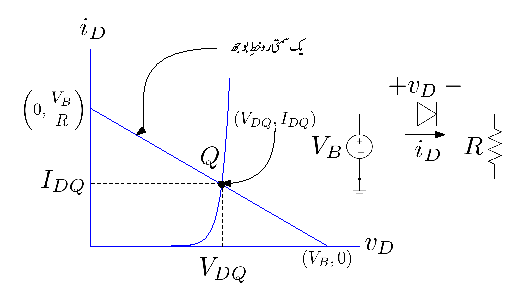
\includegraphics[scale=0.90]{diodeDCloadLine}
\caption{ برقی بار کا خط اور نقطہِ مائل}
\label{شکل_ڈایوڈ_بار_کا_خط}
\end{figure}
	ان دو مساوات کو کئی طریقوں سے حل کر کے \عددی{i_D} اور \عددی{v_D} اصل کئے جا سکتے ہیں۔آئیں انہیں حل کرنے کے چند طریقے دیکھیں۔

\جزوحصہ{گراف کا طریقہ}
شکل \حوالہ{شکل_ڈایوڈ_بار_کا_خط} میں مساوات \حوالہ{مساوات_ڈایوڈ_بار_کا_خط}  اور مساوات  \حوالہ{مساوات_ڈایوڈ_کا_خط_جس_پر_بار_لدا_جائے} کو گراف کیا گیا ہے۔جس نقطے پر دونوں مساوات کے خط ٹکراتے ہیں یہی ان کا حل ہے یعنی \عددی{\left ( V_{DQ},I_{DQ}\right )}۔ اس نقطے کو \موٹا{یک سمتی نقطہِ مائل}\فرہنگ{یک سمتی!نقطہ مائل}\فرہنگ{DC bias point}\حاشیہب{DC bias point} یا \موٹا{یک سمتی نقطہ کارکردگی}\فرہنگ{یک سمتی!نقطہ کارکردگی}  کہتے ہیں۔ان ناموں کو عموماً چھوٹا کر کے \موٹا{نقطہِ مائل} یا \موٹا{نقطہِ کارکردگی} پکارتے ہیں۔نقطہ کارکردگی کو \عددی{Q} سے ظاہر کیا جاتا ہے۔

شکل \حوالہ{شکل_ڈایوڈ_بار_کا_خط} میں مساوات  \حوالہ{مساوات_ڈایوڈ_بار_کا_خط} کے خط کو \موٹا{یک سمتی بار کا خط}\حاشیہد{گھوڑے پر بار لادا جاتا ہے۔یہاں \عددی{R} بطور برقی بار کردار ادا کرتا ہے اور اس کے مساوات کے گراف کو \موٹا{بار کا خط} کہتے ہیں}\فرہنگ{یک سمتی!بار کا خط}\فرہنگ{بار کا خط!یک سمتی}\فرہنگ{DC load line}\حاشیہب{DC load line} کہا گیا ہے۔اس نام کو چھوٹا کر کے اسے \موٹا{بار کا خط}  بھی کہتے ہیں۔آئیں اس خط پر غور کرتے ہیں۔بار کے خط کی \موٹا{ڈھلوان}\فرہنگ{ڈھلوان}\فرہنگ{gradient}\حاشیہب{gradient}
\begin{align*}
\frac{\Delta i_D}{\Delta v_D}=-\frac{1}{R}
\end{align*}
کے برابر ہے۔بار کا خط افقی محور یعنی برقی دباو \عددی{v_D} کے محور کو \عددی{(V_B,0)} پر ٹکراتا ہے جبکہ عمودی محور یعنی برقی رو \عددی{i_D} کے محور کو  \عددی{\left(0,\tfrac{V_B}{R} \right)} پر ٹکراتا ہے۔

یوں اگر مزاحمت برقرار رکھتے ہوئے دور میں داخلی برقی دباو \عددی{V_B} کی قیمت بڑھا کر \عددی{V_{B1}} کر دی جائے تو بار کا خط افقی محور کو موجودہ جگہ سے قدرِ دائیں جانب \عددی{(V_{B1},0)} پر ٹکرائے گا اور عمودی محور کو  \عددی{(0,\tfrac{V_{B1}}{R})}  پر ٹکرائے گا۔

شکل \حوالہ{شکل_داخلی_برقی_دباو_کا_بار_کے_خط_پر_اثر}  میں بار کے خطوط کو داخلی برقی  \عددی{V_B} اور \عددی{V_{B1}} کے لئے گراف کیا گیا ہے۔آپ دیکھ سکتے ہیں کہ بیرونی برقی دباو \عددی{V_B}بڑھانے سے  بار کے خط کا ڈھلوان تبدیل نہیں ہوتا اور یوں دونوں خطوط آپس میں متوازی ہوتے ہیں۔
\begin{figure}
\centering
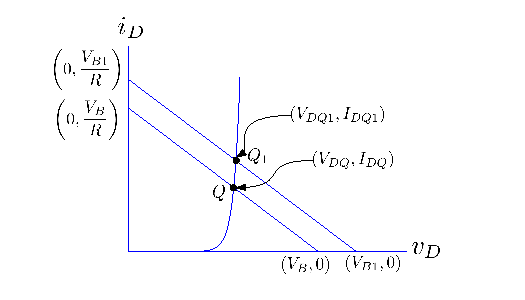
\includegraphics[scale=0.90]{DCloadLineVersusInputVoltage}
\caption{داخلی برقی دباو کا بار کے خط پر اثر}
\label{شکل_داخلی_برقی_دباو_کا_بار_کے_خط_پر_اثر}
\end{figure}
اس کے برعکس اگر بیرونی برقی دباو \عددی{V_B} برقرار رکھی جائے اور مزاحمت \عددی{R_1} کر دیا جائے تو بار کے خط کا ڈھلوان تبدیل ہو گا جبکہ یہ اب بھی محورِ برقی دباو کو \عددی{\left(V_B,0 \right)} پر ٹکرائے گا۔محورِ برقی رو سے ٹکرانے کا مقام تبدیل ہو کر \عددی{\left(0,\tfrac{V_B}{R_1} \right)} ہو جائے گا۔شکل \حوالہ{شکل_مزاحمت_کا_بار_کے_خط_پر_اثرات}  میں اس صورت کو دکھایا گیا ہے جہاں مزاحمت کی نئی قیمت \عددی{R_1} کو اس کی پرانی قیمت \عددی{R} سے کم تصور کیا گیا ہے۔
\begin{figure}
\centering
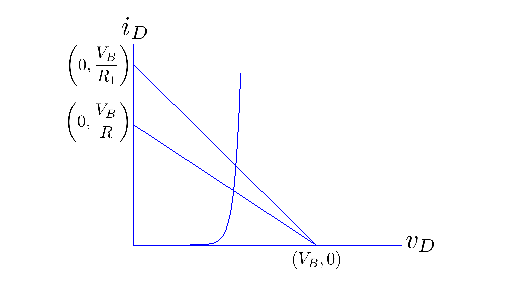
\includegraphics[scale=0.90]{DCloadLineVersusResistance}
\caption{مزاحمت کی تبدیلی کا بار کے خط پر اثر}
\label{شکل_مزاحمت_کا_بار_کے_خط_پر_اثرات}
\end{figure}
\جزوحصہ{دہرانے کا طریقہ}
عموماً مساوات \موٹا{دہرانے کے طریقے}\فرہنگ{دہرانے کا طریقہ}\فرہنگ{iteration method}\حاشیہب{iteration method}  سے با آسانی حل کئے جاتے ہیں۔موجودہ مسئلہ بھی کچھ اسی نوعیت کا ہے اور اسے بھی دہرانے کے طریقے سے نپٹا جا سکتا ہے۔اس طریقے کو مثال کی مدد سے دیکھتے ہیں۔

%===========
\ابتدا{مثال}
شکل \حوالہ{شکل_ڈایوڈ_بار_کا_خط}  میں \عددی{V_B=\SI{15}{\volt}} اور \عددی{R=\SI{15}{\kilo \ohm}} ہیں۔اگر اس ڈایوڈ
 میں \عددی{V_D=\SI{0.6}{\volt}} پر \عددی{I_D=\SI{2}{\milli \ampere}} برقی رو گزرتا ہے تو اس دور میں برقی رو حاصل کریں۔ 

حل:	مساوات \حوالہ{مساوات_ڈایوڈ_کا_خط_جس_پر_بار_لدا_جائے}  سے
\begin{align*}
I_S = \frac{i_D}{\left( e^{\frac{v_D}{V_T}} \right )}=\frac{2 \times 10^{-3}}{e^{\frac{0.6}{0.025}}}=\SI{7.550269e-14}{\ampere}
\end{align*}
حاصل ہوتا ہے۔ہمیں قبل از وقت ڈایوڈ کی برقی رو یا اس پر برقی دباو معلوم نہیں مگر دئے گئے معلومات سے ہم یہ اخذ کر سکتے ہیں کہ اگر برقی رو دو ملی ایمپیئر کے قریب ہو تو برقی دباو اشاریہ چھ وولٹ کے قریب ہو گا۔

\عددی{\SI{2}{\milli \ampere}} کو \عددی{I_{D_0}} لکھتے ہوئے (یعنی \عددی{I_{D_0}=\SI{2}{\milli \ampere}}) اور
 \عددی{\SI{0.6}{\volt}} کو  \عددی{V_{D_0}} لکھتے ہوئے (یعنی \عددی{V_{D_0}=\SI{0.6}{\volt}}) ہم سوال حل کرتے ہیں۔طریقہ کار کچھ یوں ہے کہ ہم اخذ کریں گے کہ ڈایوڈ پر  \عددی{V_{D_0}} برقی دباو ہے۔اس قیمت کو استعمال کرتے ہوئے مساوات \حوالہ{مساوات_ڈایوڈ_بار_کا_خط}  کی مدد سے ہم برقی رو حاصل کریں گے جسے ہم \عددی{I_{D_1}} کہیں گے۔مساوات \حوالہ{مساوات_ڈایوڈ_کا_خط_جس_پر_بار_لدا_جائے}  میں \عددی{I_{D_1}} کی قیمت استعمال کرتے ہوئے ڈایوڈ پر برقی دباو حاصل کیا جائے گا جسے ہم \عددی{V_{D_1}} کہیں گے۔

ڈایوڈ پر \عددی{V_{D_0}} برقی دباو اس صورت ہوتا جب اس میں \عددی{I_{D_0}} برقی رو گزرتی جبکہ ہم دیکھ سکتے ہیں کہ اصل دور میں برقی رو \عددی{I_{D_1}} کے قریب ہو گی اور یوں \عددی{I_{D_1}} کے نسبت سے حاصل شدہ برقی دباو \عددی{V_{D_1}} اصل قیمت کے زیادہ قریب برقی دباو ہو گا۔یوں اگر  \عددی{V_{D_1}} استعمال کرتے ہوئے یہ سارا سلسلہ دوبارہ دہرایا جائے یعنی مساوات \حوالہ{مساوات_ڈایوڈ_بار_کا_خط}  میں \عددی{V_{D_1}}  استعمال کرتے ہوئے \عددی{I_{D_2}} حاصل کیا جائے تو حاصل برقی رو مزید بہتر جواب ہو گا اور اگر مساوات \حوالہ{مساوات_ڈایوڈ_کا_خط_جس_پر_بار_لدا_جائے}  میں \عددی{I_{D_2}} استعمال کرتے ہوئے \عددی{V_{D_2}} حاصل کیا جائے تو یہ \عددی{V_{D_1}} سے بہتر جواب ہو گا۔ اس طریقے کو اس وقت تک  دہرایا جاتا ہے جب تک حاصل قیمتوں میں تبدیلی قابلِ نظر انداز ہو جائے۔آئیں دہرانے کے اس طریقے کو استعمال کریں۔
 
مساوات \حوالہ{مساوات_ڈایوڈ_بار_کا_خط}  میں \عددی{V_{D_0}=\SI{0.6}{\volt}} استعمال کرنے سے
\begin{align*}
I_{D_1}=\frac{V_B-V_{D_0}}{R}=\frac{15-0.6}{15000}=\SI{0.96}{\milli \ampere}
\end{align*}
اور مساوات \حوالہ{مساوات_ڈایوڈ_کا_خط_جس_پر_بار_لدا_جائے}  میں \عددی{I_{D_1}} کے استعمال سے
\begin{align*}
V_{D_1}=V_T \ln \frac{I_{D_1}}{I_S}=0.025 \times \ln \left (\frac{0.96 \times 10^{-3}}{7.550269 \times 10^{-14}} \right )=\SI{0.58165077}{\volt}
\end{align*}
یہ برقی دباو گزشتہ اخذ کردہ قیمت سے زیادہ درست قیمت ہے لہٰذا اس کو استعمال کرتے ہوئے ہم ایک مرتبہ پھر مساوات \حوالہ{مساوات_ڈایوڈ_بار_کا_خط} حل کرتے ہیں۔
\begin{align*}
I_{D_2}=\frac{15-0.58165}{15000}=\SI{0.9612233}{\milli \ampere}
\end{align*}
یہ جواب بالکل درست تب ہوتا اگر \عددی{\SI{0.9612233}{\milli \ampere}} پر ڈایوڈ کا برقی دباو \عددی{\SI{0.58165077}{\volt}} ہوتا مگر ایسا نہیں ہے لہٰذا ہمیں ایک مرتبہ پھر ڈایوڈ کے برقی دباو کا بہتر اندازہ لگانا ہو گا۔یوں \عددی{\SI{0.9612233}{\milli \ampere}} کو \عددی{I_{D_2}} اور  ڈایوڈ پر برقی دباو کو \عددی{V_{D_2}} لیتے ہوئے۔
\begin{align*}
V_{D_2}=V_T \ln \frac{I_{D_2}}{I_S}=-0.025 \times \ln \left ( \frac{0.9612233 \times 10^{-3}}{7.550269 \times 10^{-14}} \right )=\SI{0.58168261}{\volt}
\end{align*}
حاصل ہوتا ہے۔اور اس نئی قیمت کو استعمال کرتے ہوئے
\begin{align*}
I_{D_3}=\frac{V_B-V_{D_2}}{R}=\frac{15-0.58168261}{15000}=\SI{0.9612211}{\milli \ampere}
\end{align*}
حاصل ہوتا ہے۔ہم دیکھتے ہیں کہ گزشتہ دو حاصل جواب یعنی\عددی{I_{D_2}=\SI{0.9612233}{\milli \ampere}}  اور \عددی{I_{D_3}=\SI{0.9612211}{\milli \ampere}} تقریباً برابر ہیں۔ایسا ہونا اس بات کی نشانی ہے کہ جواب اصل جواب کے بہت قریب ہے اور یوں \عددی{I_{D_4}=\SI{0.96122}{\milli \ampere}} کو ہم درست جواب تسلیم کر لیتے ہیں۔

\انتہا{مثال}

%=======

\حصہ{کارتیسی محدد اور ترسیم}\label{حصہ_کارتیسی_محدد_اور_ترسیم}
اس حصے میں کارتیسی محدد  اور ترسیم پر غور کیا جائے گا جس کی اس کتاب میں کئی جگہ ضرورت پیش آئے گی۔اگرچہ اس حصے کو کتاب کے آخر میں ضمیمہ کے طور رکھنا چاہئے تھا مگر اس کی اہمیت کو دیکھتے ہوئے میں نے اسے اس باب کا حصہ بنا لیا ہے۔طلبہ سے گزارش کی جاتی ہے کہ وہ اس حصے کو بخوبی سمجھیں۔
\جزوحصہ{محدد کی منتقلی}  \شناخت{حصہ_ڈایوڈ_محدد_کی_منتقلی}
شکل \حوالہ{شکل_کارتیسی_محدد} الف میں دو کارتیسی محدد  دکھائے گئے ہیں۔ \عددی{(x-y)} کارتیسی محدد  میں دو نقطے \عددی{P(6,8)} اور \عددی{Q(4,6)} دکھائے گئے ہیں۔\عددی{(x' - y')} محدد میں یہی نقطے \عددی{P'(2,2)} اور \عددی{Q'(0,0)} بن جاتے ہیں۔
\begin{figure}
\centering
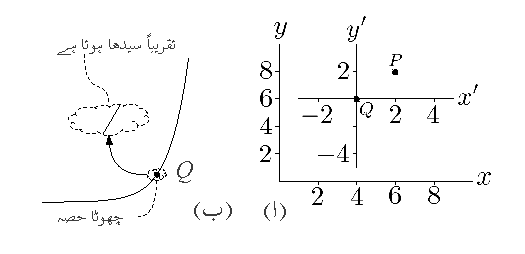
\includegraphics[scale=0.90]{cartesianCoordinates}
\caption{ (ا) کارتیسی محدد۔  (ب) خط کے چھوٹے حصے کا سیدھا پن}
\label{شکل_کارتیسی_محدد}
\end{figure}
\جزوحصہ{خط کا چھوٹا حصہ سیدھا تصور کیا جا سکتا ہے} \شناخت{حصہ_ڈایوڈ_چھوٹا_حصہ_کے_سیدھا_پن}
شکل \حوالہ{شکل_کارتیسی_محدد} ب میں یہ حقیقت دکھایا گیا ہے کہ کسی بھی خط کے چھوٹے سے حصے کو سیدھا تصور کیا جا سکتا ہے۔اگر کبھی آپ کسی خط کا چھوٹا حصہ لیں اور آپ کو لگے کہ یہ چھوٹا حصہ سیدھا تصور کرنے کے قابل نہیں ہے تو اس سے مزید چھوٹا حصہ لیجئے۔اس شکل میں چھوٹے بلبلے میں گھیرے خط کو بڑھے بلبلے میں بڑھا چڑھا کر دکھایا گیا ہے جہاں اس کا سیدھا پن صاف واضح ہے۔

\جزوحصہ{گراف سے قیمت حاصل کرنے کا عمل}
شکل \حوالہ{شکل_وقت_کے_ساتھ_تبدیل_ہوتے_متغیرات} ب کے گراف سے مختلف \عددی{x}   پر\عددی{y(x)}  کی قیمت حاصل کر کے انہیں جدول \حوالہ{جدول_گراف_سے_حاصل_کی_گئی_قیمتیں}  میں دکھایا گیا ہے۔آپ گراف سے قیمت حاصل کرنے کے اس عمل سے بخوبی واقف ہیں۔اس شکل میں \عددی{y(x)}  خم دار خط ہے۔
\begin{table} [h]
\caption{گراف سے حاصل کی گئی قیمتیں}
\label{جدول_گراف_سے_حاصل_کی_گئی_قیمتیں}
\centering
\begin{LTR}
\begin{tabular}{c|c c c c c c}
x & 0 & 1 & 2 & 3 & 4 & 5 \\
\midrule
y & 0 & 0.03 & 0.12 & 0.44 & 1.49 & 4.99 \\
\end{tabular}
\end{LTR}

\end{table}


\begin{figure}
\centering
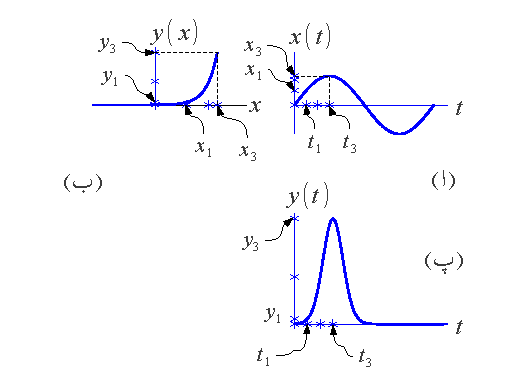
\includegraphics[scale=0.90]{timeVaryingSignals}
\caption{ وقت کے ساتھ بدلتے متغیرات کی مثال}
\label{شکل_وقت_کے_ساتھ_تبدیل_ہوتے_متغیرات}
\end{figure}
اب تصور کریں کہ \عددی{x(t)} وقت کے ساتھ تبدیل ہوتا تفاعل ہے اور ہم چاہتے ہیں کہ وقت کے ساتھ \عددی{y(t)}  کی تبدیلی گراف کریں۔ \عددی{x(t)} کے وقت کے ساتھ گراف کی شکل کچھ بھی ہو سکتی ہے۔شکل \حوالہ{شکل_وقت_کے_ساتھ_تبدیل_ہوتے_متغیرات} الف میں \عددی{x(t)} کوسائن نما تصور کیا گیا ہے۔


شکل  \حوالہ{شکل_وقت_کے_ساتھ_تبدیل_ہوتے_متغیرات} الف میں مختلف اوقات مثلاً  \عددی{t_0,t_1,t_2,\ \dots t_n} پر \عددی{x_0,x_1,x_2\dots x_n} کی قیمت حاصل کریں جہاں \عددی{x_0}  سے مراد \عددی{t_0} پر \عددی{x} کی قیمت یعنی \عددی{x(t_0)} ہے۔\عددی{t_0} تا \عددی{t_n} نقاط کی کُل تعداد  یعنی \عددی{\left(n+1 \right)}  کا تعین آپ جیسے اور جتنی چاہیں کر سکتے ہیں۔اسی طرح کسی دو قریبی نقاط کے مابین فاصلہ مثلاً
\begin{align*}
\Delta t_2=t_3 -t_2
\end{align*}
آپ جتنی چاہیں رکھ سکتے ہیں۔اس کے علاوہ کسی دو قریبی نقاط کے درمیان فاصلہ مثلاً 
\begin{align*}
\Delta t_5=t_6-t_5
\end{align*}
اور کسی اور دو قریبی نقاط کے درمیان فاصلہ  مثلاً
\begin{align*}
\Delta t_8=t_9-t_8
\end{align*}
ایک دونوں سے مختلف ہو سکتے ہیں۔اس طرح آپ کے پاس جدول \حوالہ{جدول_ایکس_بالمقابل_ٹی} حاصل ہو گا۔
\begin{table} [h]
\caption{\عددی{x(t)} بالمقابل \عددی{t}  کا جدول}
\label{جدول_ایکس_بالمقابل_ٹی}
\centering
\begin{LTR}
\begin{tabular}{c c c c c }
$ t_0 $ & $ t_1 $ & $ t_2 $ & $\cdots$ & $ t_n $ \\
\midrule
$ x_0 $ & $ x_1 $ & $ x_2 $ & $\cdots$ & $ x_n $ \\
\end{tabular}
\end{LTR}
\end{table}

جدول \حوالہ{جدول_ایکس_بالمقابل_ٹی} میں دئے \عددی{x} پر شکل \حوالہ{شکل_وقت_کے_ساتھ_تبدیل_ہوتے_متغیرات} ب سے \عددی{y} کے قیمتیں حاصل کریں۔یوں آپ کے پاس \عددی{y_0,y_1,y_2,\dots y_n} حاصل ہوں گے۔ان قیمتوں کو استعمال کرتے ہوئے \عددی{y(t)} بالمقابل \عددی{t} کا جدول \حوالہ{جدول_وائے_بالمقابل_ٹی} حاصل ہو گا جسے شکل \حوالہ{شکل_وقت_کے_ساتھ_تبدیل_ہوتے_متغیرات} پ کی طرح گراف کریں۔
\begin{table} [h]
\caption{\عددی{y(t)} بالمقابل \عددی{t}  کا جدول}
\label{جدول_وائے_بالمقابل_ٹی}
\centering
\begin{LTR}
\begin{tabular}{c c c c c }
$ t_0 $ & $ t_1 $ & $ t_2 $ & $\cdots$ & $ t_n $ \\
\midrule
$ y_0 $ & $ y_1 $ & $ y_2 $ & $\cdots$ & $ y_n $ \\
\end{tabular}
\end{LTR}
\end{table}
یہاں میں بتلانا چاہوں گا کہ اس مثال میں تفاعل \عددی{y(x)} \موٹا{خم دار}\فرہنگ{خم دار}\حاشیہب{curved}  تھا۔اس کو استعمال کرتے ہوئے تفاعل \عددی{x(t)} سے تفاعل \عددی{y(t)} حاصل کی گئی۔ \عددی{x(t)} اور \عددی{y(t)} کی شکلیں بالکل مختلف ہیں۔

مندرجہ بالا تمام عمل کو نہایت عمدگی اور نسبتاً زیادہ آسانی کے ساتھ بھی سرانجام دیا جا سکتا ہے۔آئیں اس بہتر طریقے کو شکل \حوالہ{شکل_سیدھا_تفاعل_شکل_برقرار}  کی مدد سے دیکھیں جہاں بدلتے اشارہ \عددی{x(t)} کو شکل \حوالہ{شکل_سیدھا_تفاعل_شکل_برقرار} الف میں گھما کر دکھایا گیا ہے۔ اس مثال میں بھی  \عددی{x(t)} کو سائن نما تصور کیا گیا ہے جبکہ  تفاعل \عددی{y(x)} کو سیدھا خط یعنی
\begin{align} \label{مساوات_محور_سے_گزرتا_سیدھا_خط}
y(x)= m x
\end{align}
تصور کرتے ہوئے شکل  ب میں دکھایا گیا ہے۔\حاشیہد{سیدھے خط کی مساوات \عددی{y=mx+c} ہے جہاں \عددی{c} وہ نقطہ ہے جہاں خط \عددی{y} محور کو کاٹتا ہے۔سیدھا خط \عددی{(0,0)} سے گزرنے کی صورت میں \عددی{c=0} ہو گا اور یوں سیدھے خط کی مساوات \عددی{y=mx} ہو گی۔} جیسے کہ آپ آگے دیکھیں گے، سیدھا \عددی{y(x)} نہایت اہمیت کا حامل ہے اور اس موقع سے فائدہ اٹھاتے ہوئے ہم اسی کو استعمال کرتے ہوئے آگے بڑھتے ہیں۔مساوات \حوالہ{مساوات_محور_سے_گزرتا_سیدھا_خط}   میں \عددی{m} شکل \حوالہ{شکل_کارتیسی_محدد} ب میں نقطہ \عددی{Q} پر خط کے چھوٹے سیدھے حصے کی ڈھلوان ہے یعنی 
\begin{align} \label{مساوات_ڈایوڈ_سیدھے_خط_کی_ڈھلوان_الف}
m=\left . \frac{\partial y}{\partial x} \right|_Q
\end{align}
%
\begin{figure}
\centering
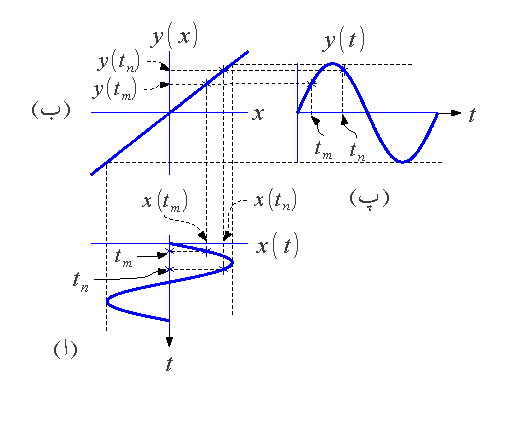
\includegraphics[scale=0.90]{linearFunctionMaintainsSignalShape}
\caption{سیدھا تفاعل اشارے کی شکل برقرار رکھتا ہے }
\label{شکل_سیدھا_تفاعل_شکل_برقرار}
\end{figure}
شکل \حوالہ{شکل_سیدھا_تفاعل_شکل_برقرار} الف میں دو نقطے \عددی{t_m} اور \عددی{t_n}  کو مثال بناتے ہوئے پورے عمل کو سمجھایا گیا ہے۔ان دو نقطوں پر \عددی{x(t_m)} اور \عددی{x(t_n)} حاصل کئے جاتے ہیں۔ان کی قیمت جاننا ضروری نہیں، بس اتنا درکار ہے کہ ان کی نشاندہی گراف پر کر دی جائے۔

شکل  الف اور شکل  ب یوں بنائے جاتے ہیں کہ شکل  ب کا \عددی{x} محدد شکل  الف کے \عددی{x} محدد کے متوازی ہو اور ان کی جسامت بھی برابر ہو۔یوں شکل  الف میں \عددی{x(t_m)} اور \عددی{x(t_n)} سے سیدھی لکیریں شکل  ب تک لے جائیں ۔اس طرح شکل  ب سے \عددی{y(t_m)} اور \عددی{y(t_n)}حاصل ہوں گے۔

شکل  ب اور شکل  پ یوں بنائے جاتے ہیں کہ شکل  پ کا \عددی{y} محدد شکل  ب کے \عددی{y} محدد کے بالکل دائیں جانب برابر رکھا جائے اور ان کی جسامت بھی برابر ہو۔یوں شکل  ب کے \عددی{y(t_m)} اور \عددی{y(t_n)} نقطوں سے شکل  پ تک افقی لکیریں بنائیں۔شکل  پ پر ان نقطوں کو وقت \عددی{t_m} اور \عددی{t_n} کے ساتھ گراف کریں۔مندرجہ بالا پورا عمل شکل  \حوالہ{شکل_سیدھا_تفاعل_شکل_برقرار}  کو دیکھتے ہی ایک دم سمجھ آ جانا چاہئے۔

شکل \حوالہ{شکل_سیدھا_تفاعل_شکل_برقرار}  میں \عددی{y(x)} ایک خطی ( یعنی غیر-خم دار ) تفاعل ہے۔اسے استعمال کرتے ہوئے شکل  پ حاصل کی گئی۔شکل  پ اور شکل  الف ہو بہو ایک ہی طرح ہیں۔ان کے صرف حیطے مختلف ہو سکتے ہیں۔یہ ایک نہایت اہم نتیجہ ہے جس کا برقیات کے میدان میں کلیدی کردار ہے۔اس حقیقت کو استعمال کرتے ہوئے غیر-خم دار تفاعل کے اشکال میں چونکہ صرف حیطہ تبدیل ہوتا ہے لہٰذا عموماً اشارہ  \عددی{x(t)}  کے چوٹیوں سے شکل  ب تک اور یہاں سے شکل  پ تک لکیریں کھینچ کر شکل  پ مکمل کر دیا جاتا ہے۔

شکل \حوالہ{شکل_وقت_کے_ساتھ_تبدیل_ہوتے_متغیرات}  اور شکل \حوالہ{شکل_سیدھا_تفاعل_شکل_برقرار}  میں \عددی{x(t)} کو داخلی ( یا اصل ) اشارہ ، \عددی{y(t)} کو خارجی ( یا منعکس\حاشیہب{image}) اشارہ جبکہ \عددی{y(x)}  کو آئینہ\حاشیہب{mirror} تصور کریں۔یوں ہم کہہ سکتے ہیں کہ غیر-خم دار آئینے میں اشارے کی شکل جوں کی توں رہتی ہے جبکہ خم دار آئینہ شکل بگاڑ دیتا ہے۔
\begin{figure}
\centering
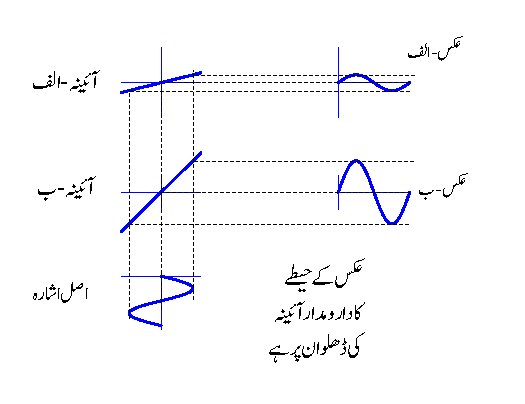
\includegraphics[scale=0.90]{mirrorSlopeVersusSignalAmplitude}
\caption{عکس کا حیطہ بالمقابل آئینے کی ڈھلوان}
\label{شکل_عکس_کا_حیطہ_بالمقابل_ڈھلوان}
\end{figure}
شکل \حوالہ{شکل_عکس_کا_حیطہ_بالمقابل_ڈھلوان}  میں آئینہ کی ڈھلون کا عکس کے حیطے پر اثر دکھایا گیا ہے۔ آئینہ  الف کی ڈھلوان آئینہ  ب کی ڈھلوان سے زیادہ ہے۔جیسے آپ دیکھ سکتے ہیں کہ آئینے کی ڈھلوان بڑھانے سے عکس کا حیطہ بڑھتا ہے جبکہ آئینہ کی ڈھلوان گھٹانے سے عکس کا حیطہ گھٹتا ہے۔آئینے کی ڈھلوان یوں بھی رکھی جا سکتی ہے کہ عکس کے حیطے میں کوئی تبدیلی پیدا نہ ہو اور یہ اصل اشارہ کے حیطے کے برابر ہی رہے۔

مندرجہ بالا تذکرہ کو تحلیلی جامہ پہناتے ہیں۔مساوات \حوالہ{مساوات_محور_سے_گزرتا_سیدھا_خط}  میں \عددی{x(t)}  لکھتے ہوئے اس مساوات کو یوں لکھا جا سکتا ہے۔
\begin{gather}
\begin{aligned}[t]
y [x(t)]&=m x(t)\\
y(t)&=m x(t)
\end{aligned}
\end{gather}
اس مساوات کے تحت \عددی{y(t)} کا حیطہ \عددی{x(t)} کے حیطے کا \عددی{m} گنا ہو گا جہاں \عددی{m} آئینہ کی ڈھلوان ہے۔

برقیات کے میدان میں برقی دباو \عددی{v}  اور برقی رو \عددی{i}  کا استعمال ہوتا ہے۔روایتی طور پر برقی دباو کو \عددی{x(t)} جبکہ برقی رو کو \عددی{y(t)} تصور کیا جاتا ہے۔شکل \حوالہ{شکل_ڈایوڈ_کا_باریک_اشاراتی_مزاحمت}  میں ایسا دکھایا گیا ہے۔آپ جانتے ہیں کہ  یک سمتی برقی دباو تقسیمِ یک سمتی برقی رو کو مزاحمت \عددی{R} جبکہ یک سمتی برقی رو تقسیمِ یک سمتی برقی دباو کو موصلیت \عددی{G} لکھا جاتا ہے۔مزید یہ کہ باریک اشاراتی مزاحمت کو \عددی{r} جبکہ باریک اشاراتی موصلیت کو \عددی{g} لکھا جاتا ہے۔یوں مساوات \حوالہ{مساوات_ڈایوڈ_سیدھے_خط_کی_ڈھلوان_الف}   میں چھوٹے ( یعنی باریک ) سیدھے حصے کی ڈھلون  \عددی{m} کی جگہ باریک اشاراتی موصلیت \عددی{g}  کا استعمال ہو گا۔یوں مساوات \حوالہ{مساوات_محور_سے_گزرتا_سیدھا_خط}  کو برقیات کے میدان میں استعمال کرتے وقت مندرجہ ذیل طرز پر لکھا جائے گا۔

\begin{align} \label{مساوات_موصلیت_نما_کے_استعمال_سے_رو_کا_حصول}
i(t)= g v(t)
\end{align}
اسی طرح مساوات \حوالہ{مساوات_ڈایوڈ_سیدھے_خط_کی_ڈھلوان_الف}  کو یوں لکھا جائے گا
\begin{align} \label{مساوات_موصلیت_نما_کی_تعریف}
g = \left .  \frac{\partial  i}{\partial v} \right |_Q
\end{align}
اور باریک اشاراتی مزاحمت \عددی{r} کے لئے یوں لکھا جائے گا۔
\begin{align}
r=\left . \frac{\partial i}{\partial v} \right|_Q ^{-1}
\end{align}

\begin{figure}
\centering
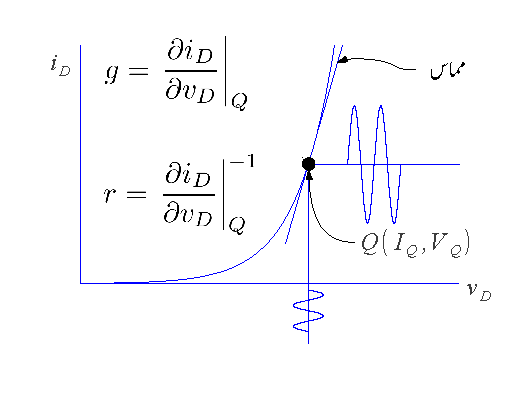
\includegraphics[scale=0.90]{smallSignalConductanceAndResistanceDiode}
\caption{ باریک اشاراتی موصلیت اور باریک اشاراتی مزاحمت}
\label{شکل_ڈایوڈ_کا_باریک_اشاراتی_مزاحمت}
\end{figure}
\حصہ{باریک اشاراتی تجزیہ} \label{حصہ_باریک_اشاراتی_تجزیہ}
شکل \حوالہ{شکل_باریک_اشارہ} الف میں داخلی برقی دباو \عددی{v_I} استعمال کی گئی ہے۔گراف میں   \عددی{v_I}  کی قیمت مثبت رہتے ہوئے مسلسل تبدیل ہوتی دکھائی گئی ہے۔جیسا شکل  ب میں دکھایا گیا ہے، \عددی{v_I}  کو یوں بھی تصور کیا جا سکتا ہے کہ اسے یک سمتی برقی دباو  \عددی{V_I} اور بدلتے برقی دباو  \عددی{v_i} کو سلسلہ وار جوڑ کر حاصل کیا گیا ہے یعنی
\begin{align}
v_I = V_I+v_i
\end{align}
%
\begin{figure}
\centering
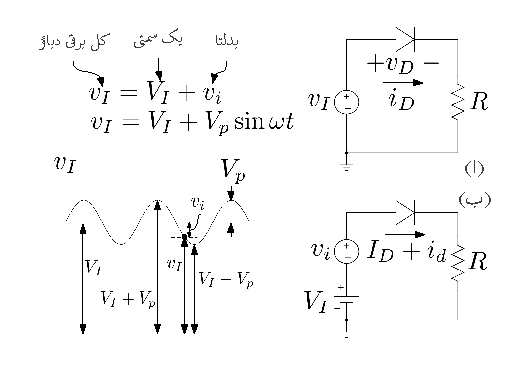
\includegraphics[scale=0.90]{smallSignalDetails}
\caption{باریک اشارہ}
\label{شکل_باریک_اشارہ}
\end{figure}

\موٹا{باریک اشارہ}\فرہنگ{باریک اشارہ}\فرہنگ{small signal}\حاشیہب{small signal}  سے مراد وہ بدلتا اشارہ ہے جس کا حیطہ دور میں پائے جانے والے یک سمتی برقی دباو یا  یک سمتی برقی رو کی قیمتوں سے نہایت کم ہو ( یعنی \عددی{v_i << V_I} )۔

شکل \حوالہ{شکل_داخلی_برقی_دباو_کا_بار_کے_خط_پر_اثر}  میں تغیر پذیر داخلی برقی دباو کا بار کے خط پر اثر دکھایا گیا۔اسی ترکیب کو یہاں استعمال کرتے ہوئے باریک داخلی اشارہ \عددی{v_i}  کی موجودگی میں ڈایوڈ کی کارکردگی پر غور کیا جائے گا۔تغیر پذیر داخلی برقی دباو \عددی{v_I}  سے نپٹنے کی خاطر مختلف لمحات پر وقت کو ساکن تصور کرتے ہوئے ان لمحات پر داخلی برقی دباو کی کل قیمت لی جاتی ہے۔ان قیمتوں پر بار کے خط اور ڈایوڈ کی مساوات کا خط گراف کیا جاتا ہے۔یوں مختلف اوقات پر ڈایوڈ کے مختلف نقطہ مائل \عددی{(V_{DQ},I_{DQ})}  حاصل کئے جاتے ہیں۔

شکل \حوالہ{شکل_ڈایوڈ_پر_باریک_اشارات}  میں \عددیء{\omega t_0=\SI{0}{\degree}}،   \عددیء{\omega t_0=\SI{90}{\degree}} اور  \عددیء{\omega t_0=\SI{270}{\degree}}  پر داخلی برقی دباو \عددیء{v_I(t_0)=V_I}، \عددی{v_I(t_1)=V_I+V_p} اور \عددی{v_I(t_2)=V_I-V_p} استعمال کرتے بار کے خط گراف کئے گئے ہیں۔
\begin{figure}
\centering
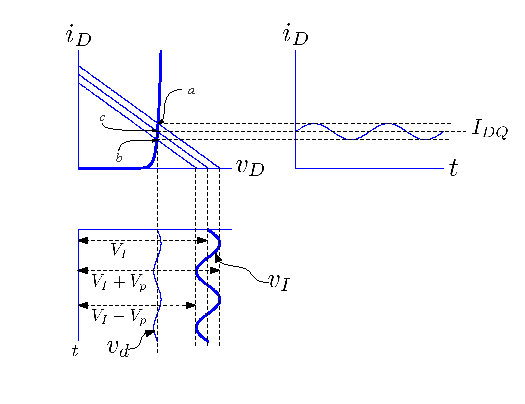
\includegraphics[scale=0.90]{smallSignalsOnDiode}
\caption{ ڈایوڈ پر باریک اشارات}
\label{شکل_ڈایوڈ_پر_باریک_اشارات}
\end{figure}
%=========================================

شکل \حوالہ{شکل_باریک_اشارہ} کے داخلی برقی دباو کے گراف کو گھڑی کی سمت  \عددیء{\SI{90}{\degree}}  کے زاویہ گھما کر شکل \حوالہ{شکل_ڈایوڈ_پر_باریک_اشارات}  میں بنایا گیا ہے۔یوں تغیر پذیر داخلی برقی دباو سے بار کے خط حاصل کرتے ہوئے دور میں بدلتی برقی رو حاصل کی جاتی ہے۔یہ  ترکیب شکل پر غور کرنے سے واضح ہو گی۔


\جزوحصہ{بدلتی رو، بار کا خط}\شناخت{حصہ_ڈایوڈ_بدلتی_رو_بار_خط}
حصہ \حوالہ{حصہ_یکسمتی_برقی_بار_کا_خط}  میں یک سمتی بار کے خط پر گفتگو کی گئی۔اسی کو آگے بڑھاتے ہوئے \موٹا{بدلتی رو، بار کے خط}\فرہنگ{بدلتی رو، بار کا خط}\فرہنگ{AC load line}\حاشیہب{AC load line}  کو یہاں پیش کیا جائے گا جس کا اگلے بابوں میں کلیدی کردار ہو گا۔
\begin{figure}
\centering
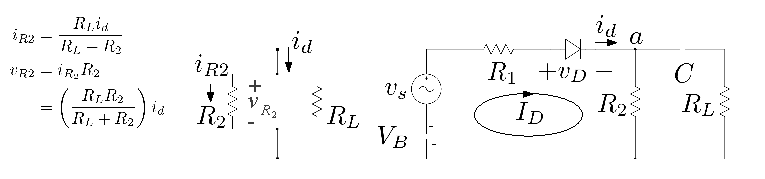
\includegraphics[scale=0.90]{ACloadLineCircuit}
\caption{ڈایوڈ کے دور میں کپیسٹر کے استعمال سے بدلتی رو، بار کا خط پیدا ہوتا ہے}
\label{شکل_ڈایوڈ_بدلتے_بار_کا_دور}
\end{figure}
شکل \حوالہ{شکل_ڈایوڈ_بدلتے_بار_کا_دور}  میں دکھائے ڈایوڈ کے دور میں کپیسٹر بھی استعمال کیا گیا ہے۔تصور کریں کہ باریک اشارہ \عددی{v_s} کے تعدد پر کپیسٹر کو قصر دور ( یعنی\عددی{\left | X_C \right | \to 0}) تصور کیا جا سکتا ہے۔چونکہ کپیسٹر میں سے یک سمتی برقی رو نہیں گزرتی لہٰذا یک سمتی برقی رو  \عددی{R_L} سے نہیں گزرے گی۔کپیسٹر کو یک سمتی متغیرات کے لئے کھلے دور تصور کیا جا سکتا ہے۔ایسا کرنے سے یک سمتی دور حاصل ہوتا ہے جس کے  یک سمتی بار کے خط کی ڈھلوان \عددی{\tfrac{-1}{R_1+R_2}} ہو گی اور \عددی{R_L }  کا اس میں کوئی کردار نہیں ہو گا۔

بدلتے اشارہ کے نقطہ نظر سے ڈایوڈ کے خارجی جانب دو متوازی جڑے مزاحمت پائے جاتے ہیں جن کی کل مزاحمت \عددی{R_t}  ہے یعنی
\begin{align}
R_t= \frac{R_L R_2}{R_L+R_2}
\end{align}
%
\begin{figure}
\centering
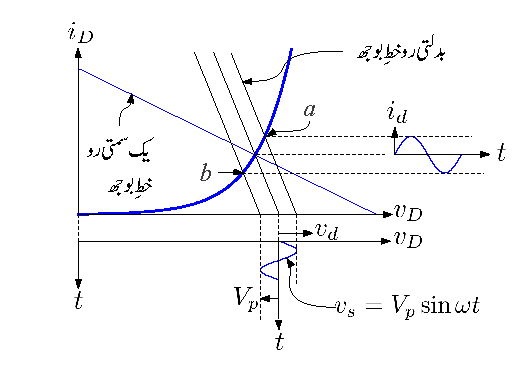
\includegraphics[scale=0.90]{diodeACloadLine}
\caption{بدلتی بار کا خط}
\label{شکل_ڈایوڈ_بدلتا_بار_کا_خط}
\end{figure}
بدلتے اشارہ کو \عددی{R_t} برقی بار دکھائی دیتا ہے۔یوں بدلتے اشارہ کے بار کے خط کی ڈھلوان \عددی{-\tfrac{1}{R_t}} ہو گی جو کہ یک سمتی بار کے خط کے ڈھلوان سے مختلف ہے۔یوں بدلتی رو، بار کا خط کھینچتے کرتے وقت اس کی ڈھلوان \عددی{-\tfrac{1}{R_t}} رکھی جائے گی۔بدلتے اشارہ کے تبدیل کے ساتھ  بدلتی رو، بار کا خط بھی جگہ تبدیل کرتا ہے۔یہ بالکل ایسا ہی ہے جیسے شکل \حوالہ{شکل_ڈایوڈ_پر_باریک_اشارات}  میں یک سمتی بار کے خط کے لئے دکھایا گیا۔چونکہ بدلتی بار کے خط کی ڈھلوان ہمیں معلوم ہے لہٰذا اسے گراف کرنے کی خاطر ہمیں مزید صرف اس پر ایک نقطہ درکار ہے۔اگر بدلتے اشارے کا حیطہ کم کرتے کرتے صفر کر دیا جائے تو یک سمتی صورتِ حال پیدا ہوتی ہے اور ہم جانتے ہیں کہ یک سمتی بار کا خط نقطہ مائل سے گزرتا ہے۔یوں صاف ظاہر ہے کہ بدلتے بار کا خط بھی نقطہ مائل سے گزرتا ہے۔شکل \حوالہ{شکل_ڈایوڈ_بدلتا_بار_کا_خط} میں دونوں بار کے خط گراف کئے گئے ہیں۔

اس طرح پہلے یک سمتی بار کا خط گراف کیا جاتا ہے جس سے نقطہ مائل حاصل کیا جاتا ہے۔نقطہ مائل سے گزرتا بدلتی رو، بار کا خط گراف کیا جاتا ہے جس کی ڈھلوان بدلتے اشارہ کے بار سے حاصل کی جاتی ہے۔بدلتے اشارہ کے موجودگی میں بدلتی رو، بار کا خط ڈایوڈ کے خط پر نقطہ \عددی{Q} کے قریب قریب رہتے ہوئے \عددی{a}  اور \عددی{b} کے درمیان چال قدمی کرتا ہے۔یہاں بھی نقطہ کارکردگی پر باریک اشارات کے لئے ڈایوڈ کے خط کو سیدھا تصور کرتے ہوئے محدد \عددی{v_d- i_d} بنائے جا سکتے ہیں جن سے\عددی{v_d} اور \عددی{i_d} کو پڑھا جا سکتا ہے۔

\عددی{v_d} اور \عددی{i_d} کو تحلیلی طریقے سے بھی حاصل کیا جا سکتا ہے۔ایسا کرنے کی خاطر شکل \حوالہ{شکل_ڈایوڈ_بدلتے_بار_کا_دور} پر غور کرتے ہیں۔اگر یہاں \عددی{v_s=0} رکھا جائے تو بائیں دائرے میں صرف یک سمتی برقی رو \عددی{I_D} گزرے گی جس سے مزاحمت \عددی{R_2} پر برقی دباو \عددی{I_D R_2} پیدا ہو گا۔یہی برقی دباو جوڑ \عددی{a} پر پایا جائے گا۔\عددی{R_L} اور کپیسٹر \عددی{C} آپس میں سلسلہ وار جڑے ہیں۔یوں ان کی برقی رکاوٹ \عددی{R_L+\tfrac{1}{j \omega C}} ہے۔یہ برقی رکاوٹ \عددی{R_2} کے متوازی جڑی ہے۔\عددیء{R_2}،\عددی{R_L} اور کپیسٹر مل کر برقی رکاوٹ \عددی{Z} پیدا کرتے ہیں جہاں
\begin{align}
\frac{1}{Z}&=\frac{1}{R_2}+\frac{1}{R_L+\frac{1}{j \omega C}}\\
Z&=\frac{R_2 \left(R_L+\frac{1}{j \omega C} \right)}{R_2+R_L+\frac{1}{j \omega C}}
\end{align}
کے برابر ہے۔کپیسٹر یک سمتی برقی رو کے لئے کھلے سرے کردار ادا کرتا ہے لہٰذا \عددی{R_L} میں یک سمتی برقی رو کی قیمت صفر ایمپیئر ہو گی اور اس پر یک سمتی برقی دباو کی قیمت بھی صفر وولٹ ہو گا۔کپیسٹر \عددی{C} جوڑ \عددی{a} پر پائے جانے والے یک سمتی برقی دباو کو برداشت کرے گا اور یوں کپیسٹر پر \عددی{V_C=I_D R_2} برقی دباو پایا جائے گا۔کرچاف کے قانون برائے برقی دباو سے لکھا جا سکتا ہے۔
\begin{align} \label{مساوات_ٹرانزسٹر_یکسمتی_سپلائی_بار_مساوات_جزو}
V_B=I_D R_1+V_D+I_D R_2
\end{align}
آئیں اب شکل \حوالہ{شکل_ڈایوڈ_بدلتے_بار_کا_دور} میں یک سمتی برقی دباو \عددی{V_B} برقرار رکھتے ہوئے \عددی{v_s} کو صفر سے بڑھایا جاتا ہے تا ہم \عددی{v_s \ll V_B} رکھا جاتا ہے۔\عددی{V_B+v_s} اب کل برقی رو \عددی{i_D=I_D+i_d} پیدا کریں گے۔\عددی{I_D} کی کہانی تبدیل نہیں ہوتی البتہ \عددی{i_d} پر غور درکار ہے۔\عددی{i_d} مزاحمت \عددی{R_1} اور ڈایوڈ سے گزرتے ہوئے جوڑ \عددی{a} پر پہنچتی ہے جہاں اسے دو راستے ملتے ہیں۔اس مثال کی خاطر کپیسٹر کو یک سمتی برقی رو کے لئے قصر دور تصور کرتے ہوئے صورت حال کو شکل میں دکھایا گیا ہے۔\عددی{i_d} کا کچھ حصہ \عددی{R_2} میں گزرے کا یعنی
\begin{align}
i_{R2}=\left(\frac{R_L}{R_L+R_2}\right) i_d
\end{align}
یوں \عددی{R_2} میں کل برقی رو کی قیمت \عددی{I_D+i_{R_2}} ہو گی۔کرچاف کے قانون برائے برقی دباو کو بائیں دائرے میں استعمال کرتے ہوئے
\begin{align*}
V_B+v_s&=i_D R_1+v_D+\left(I_D+i_{R2} \right)R_2\\
&=\left(I_D+i_d \right)R_1+ \left(V_D+v_d \right)+\left[I_D+\left(\frac{R_L}{R_L+R_2}\right) i_d \right]R_2
\end{align*}
لکھا جائے گا جہاں دوسرے قدم پر \عددی{i_D=I_D+i_d} اور \عددی{v_D=V_D+v_d} کا استعمال کیا گیا۔ اس مساوات کو دو مساوات میں یوں لکھا جا سکتا ہے۔
\begin{align} \label{مساوات_ٹرانزسٹر_یکسمتی_بدلتا_بار_کے_خط}
V_B&=I_D R_1 +V_D+I_D R_2\\
v_s&=i_d R_1+v_d+i_d \left (\frac{R_L R_2}{R_L+R_2} \right )
\end{align}
مندرجہ بالا مساوات کا پہلا جزو یک سمتی بار کے خط کی مساوات ہے جبکہ اس کا دوسرا جزو بدلتی رو بار کے خط کی مساوات ہے۔شکل \حوالہ{شکل_ڈایوڈ_بدلتے_بار_کا_دور} کو شکل \حوالہ{شکل_دور_کا_یکسمتی_اور_بدلتا_حصہ} میں دوبارہ دکھایا گیا ہے جہاں اصل دور کے ساتھ ساتھ دو مزید ادوار دکھائے گئے ہیں۔شکل \حوالہ{شکل_دور_کا_یکسمتی_اور_بدلتا_حصہ} ب میں صرف  یک سمتی سپلائی \عددی{V_B} استعمال کرتے ہوئے اصل دور کے وہ حصے دکھائے گئے ہیں جن میں یک سمتی برقی رو \عددی{I_D} گزرتی ہے۔اس میں کرچاف کے قانون برائے برقی دباو سے مساوات \حوالہ{مساوات_ٹرانزسٹر_یکسمتی_بدلتا_بار_کے_خط} کا پہلا جزو حاصل ہوتا ہے۔اسی طرح شکل \حوالہ{شکل_دور_کا_یکسمتی_اور_بدلتا_حصہ} پ میں صرف بدلتا سپلائی \عددی{v_s} استعمال کرتے ہوئے اصل دور کے وہ حصے شامل کئے گئے ہیں جن میں بدلتی برقی رو \عددی{i_d} گزرتی ہے۔اس شکل میں ڈایوڈ پر برقی دباو کو \عددی{v_d} لکھتے ہوئے اس بات کی وضاحت کی گئی ہے کہ ڈایوڈ پر بدلتے برقی دباو کی بات کی جا رہی ہے۔اس دور پر کرچاف کے قانون برائے برقی دباو سے مساوات  \حوالہ{مساوات_ٹرانزسٹر_یکسمتی_بدلتا_بار_کے_خط} کا دوسرا جزو حاصل ہوتا ہے۔
\begin{figure}
\centering
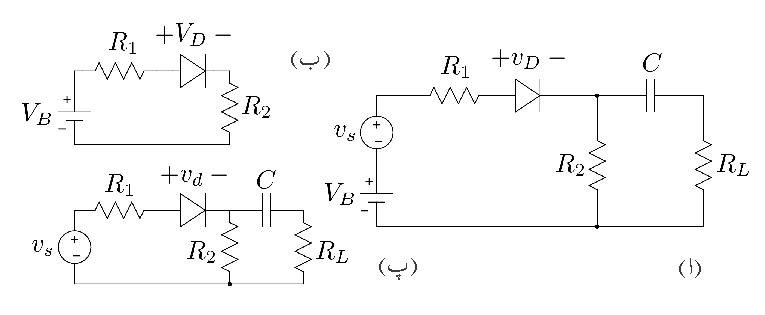
\includegraphics[scale=0.90]{ACloadLineCircuitSplitted}
\caption{دور کا یک سمتی اور بدلتے حصے میں تقسیم }
\label{شکل_دور_کا_یکسمتی_اور_بدلتا_حصہ}
\end{figure}
بدلتے بار کے خط کی مساوات میں ڈایوڈ کا باریک اشارات مزاحمت \عددی{r_d}  استعمال کرتے ہوئے \عددی{v_d=i_d r_d} لکھا جا سکتا ہے اور یوں اس خط سے \عددی{i_d}  حاصل کیا جا سکتا ہے۔
\begin{align*}
v_s&=i_d R_1+i_d r_d + i_d \left (\frac{R_L R_2}{R_L+R_2} \right )\\
i_d&=\frac{v_s}{R_1+r_d+\left (\frac{R_L R_2}{R_L+R_2} \right )}
\end{align*}
اور \عددی{v_d = i_d r_d}  کے استعمال سے \عددی{v_d}حاصل کیا جا سکتا ہے۔

یوں اصل شکل کو شکل  ب اور شکل  پ کے طرز پر بناتے ہوئے یک سمتی اور بدلتی برقی رو (اور بدلتے برقی دباو) باری باری حاصل کئے جا سکتے ہیں۔یہ نہایت اہم اور عمومی ترکیب ہے جسے برقیات کے میدان میں عموماً استعمال کیا جاتا ہے۔اس کتاب میں اس ترکیب کا بار بار استعمال کیا جائے گا۔ 

\جزوحصہ{باریک اشاراتی مزاحمت}
تغیر پذیر داخلی برقی دباو میں باریک اشارات کو نظر انداز کرتے ہوئے حاصل نقطہ مائل کو شکل \حوالہ{شکل_ڈایوڈ_پر_باریک_اشارات}  میں \عددی{c} سے ظاہر کیا گیا ہے۔باریک اشارہ کی موجودگی میں یہ نقطہ  تبدیل ہوتے ہوئے \عددی{a} اور \عددی{b} کے درمیان رہتا ہے۔ان دو نکتوں کے مابین ڈایوڈ کا خط تقریباً ایک سیدھی لکیر کی مانند ہے۔\حاشیہد{حصہ \حوالہ{حصہ_ڈایوڈ_چھوٹا_حصہ_کے_سیدھا_پن} میں دیکھا گیا کہ کسی بھی خط کے باریک حصے کو سیدھا تصور کیا جا سکتا ہے} یاد رہے کہ مزاحمت کی برقی دباو بالمقابل برقی رو کا خط سیدھی لکیر ہوتا ہے۔اگر نقطہ \عددی{c} پر \عددی{v_d - i_d} کا کارتیسی محدد بنایا جائے\حاشیہد{حصہ \حوالہ{حصہ_ڈایوڈ_محدد_کی_منتقلی} میں محدد کی منتقلی پر بحث کی گئی}  اور گراف کو \عددی{a} سے \عددی{b} تک محدود کر دیا جائے تو اس خطے میں ڈایوڈ کے مساوات کا گراف عام مزاحمت کا گراف معلوم ہوتا ہے۔شکل \حوالہ{شکل_ڈایوڈ_کے_باریک_اشارات_کا_حصول} الف کے نقطہ کارکردگی \عددی{Q}  کے قریب قریب رہتے ہوئے ڈایوڈ کے خط کو سیدھا تصور کرتے ہوئے شکل  ب میں دکھایا گیا ہے۔ یوں ان دو نکتوں کے مابین ڈایوڈ کو مزاحمت \عددی{r_d} تصور کیا جا سکتا ہے جہاں 
\begin{align} \label{مساوات_ڈایوڈ_کی_مزاحمت_الف}
r_d = \frac{v_d}{i_d}
\end{align}
شکل \حوالہ{شکل_ڈایوڈ_کے_باریک_اشارات_کا_حصول} الف میں وسیع اشاراتی محدد \عددی{(i_D  -  v_D)} جبکہ شکل \حوالہ{شکل_ڈایوڈ_کے_باریک_اشارات_کا_حصول} ب میں باریک اشاراتی محدد \عددی{(i_d  -  v_d)}  استعمال کئے گئے ہیں۔شکل  ب میں ہم یہ بھی دیکھتے ہیں کہ نقطہ کارکردگی پر ڈایوڈ کے باریک اشاراتی مزاحمت \عددی{r_d} کو استعمال کرتے ہوئے ڈایوڈ کے باریک اشاراتی برقی دباو \عددی{v_d (t)} پر اس کے باریک اشاراتی برقی رو \عددی{i_d (t)} کا خط بھی نہایت آسانی کے ساتھ حاصل کیا جا سکتا ہے۔
\begin{figure}
\centering
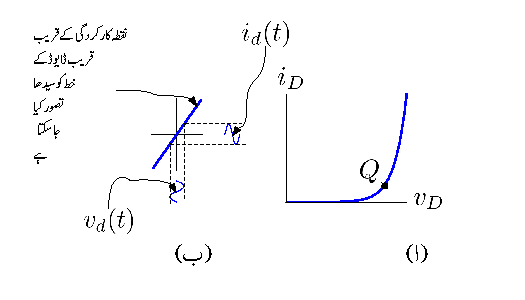
\includegraphics[scale=0.90]{diodeGraphicalSmallSignals}
\caption{ ڈایوڈ کے باریک اشارات کا حصول}
\label{شکل_ڈایوڈ_کے_باریک_اشارات_کا_حصول}
\end{figure}
باریک اشارہ کے موجودگی میں ڈایوڈ نقطہ مائل کے قریب قریب رہے گا۔ یوں اگر نقطہ \عددی{c} کو\عددی{(V_{DQ},I_{DQ})}لکھا جائے تو نقطہ \عددی{a} کو
\عددی{(V_{DQ}+\Delta V_{DQ},I_{DQ}+\Delta I_{DQ})} 
جبکہ نقطہ \عددی{b} کو
\عددی{(V_{DQ}-\Delta V_{DQ},I_{DQ}-\Delta I_{DQ})} 
لکھا جا سکتا ہے۔یوں نقطہ \عددی{c} پر ڈایوڈ کی  مزاحمت \عددی{r_d}  یوں حاصل کی جائے گی۔
\begin{align} \label{مساوات_ڈایوڈ_کی_مزاحمت_ب}
r_d = \left . \frac{\Delta v_D}{\Delta i_D} \right |_{I_{DQ}}=\frac{\Delta V_{DQ}}{\Delta I_{DQ}}
\end{align}
مساوات \حوالہ{مساوات_ڈایوڈ_کی_مزاحمت_الف}  اور مساوات \حوالہ{مساوات_ڈایوڈ_کی_مزاحمت_ب}  اس مزاحمت کو سمجھنے کے مختلف طریقے ہیں۔

\عددی{r_d} کو ڈایوڈ کا \موٹا{باریک اشاراتی مزاحمت}\فرہنگ{باریک اشاراتی!مزاحمت}\فرہنگ{small signal!resistance}\حاشیہب{small signal resistance}  کہتے ہیں اور اس کی قیمت \موٹا{نقطہ کارکردگی} پر منحصر ہے۔

\جزوحصہ{خطِ مماس سے باریک اشاراتی مزاحمت کا حصول}
شکل \حوالہ{شکل_ڈایوڈ_نقطہ_کارکردگی_پر_مماس}  میں نقطہ کارکردگی پر \موٹا{خطِ مماس}\فرہنگ{خط مماس}\حاشیہب{tangent}  دکھایا گیا ہے۔ آپ دیکھ سکتے ہیں کہ نقطہ کارکردگی پر خطِ مماس  سے ڈایوڈ کا باریک اشاراتی مزاحمت \عددی{r_d}  حاصل کیا جا سکتا ہے۔آئیں \عددی{r_d}  کو چالو ڈایوڈ کے مساوات (یعنی مساوات \حوالہ{مساوات_چالو_ڈایوڈ} ) کے خطِ مماس سے حاصل کریں۔ نقطہ کارکردگی پر چالو ڈایوڈ کا خطِ مماس حاصل کرنے کی خاطر چالو ڈایوڈ کی مساوات کا تفرق\حاشیہب{differenciation}  لیں گے۔اس تفرق کی قیمت نقطہ \عددی{i_D=I_{DQ}} پر حاصل کر کے نقطہ کارکردگی پر مزاحمت \عددی{r_d}  حاصل کی جائے گی یعنی
\begin{figure}
\centering
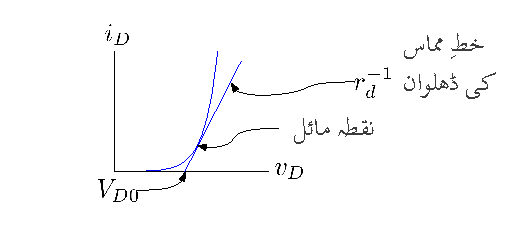
\includegraphics[scale=0.90]{tangentAtQpointDiode}
\caption{ نقطہ کارکردگی پر خطِ مماس سے باریک اشاراتی مزاحمت کا حصول}
\label{شکل_ڈایوڈ_نقطہ_کارکردگی_پر_مماس}
\end{figure}
%
\begin{gather}
\begin{aligned}[t]
i_D &=I_S \left (e^{\frac{v_D}{V_T}}-1 \right ) \approx I_S e^{\frac{v_D}{V_T}}\\
\od{i_D}{v_D}&=\frac{I_S e^{\frac{v_D}{V_T}}}{V_T}
\end{aligned}
\end{gather}
چونکہ  \عددی{i_D=I_S e^{\frac{v_D}{V_T}}}  ہے لہٰذا ہم لکھ سکتے ہیں کہ 
\begin{gather}
\begin{aligned}[t]
\od{i_D}{v_D}&=\frac{I_S e^{\frac{v_D}{V_T}}}{V_T}=\frac{i_D}{V_T}\\
\left . \od{i_D}{v_D} \right |_{I_{DQ}}&=\frac{I_{DQ}}{V_T}
\end{aligned}
\end{gather}
خطِ مماس کے اس ڈھلوان سے باریک اشاراتی مزاحمت حاصل کرتے ہیں۔
\begin{align} \label{مساوات_ڈایوڈ_کی_مزاحمت_کا_رو_سے_حصول}
r_d = \left . \left(\od{i_D}{v_D} \right )^{-1} \right|_{I_{DQ}}=\frac{V_T}{I_{DQ}}
\end{align}
%=================

\ابتدا{مثال}
ایک ڈایوڈ جس کا \عددی{I_S=\SI{9.32e-14}{\ampere}} کے برابر ہو کی   \عددی{i_D=\SI{25}{\micro \ampere}}  اور \عددی{\SI{15}{\milli \ampere}}  کی برقی رو پر باریک اشاراتی مزاحمت حاصل کریں۔

حل:	مساوات \حوالہ{مساوات_ڈایوڈ_کی_مزاحمت_کا_رو_سے_حصول}  کے تحت \عددی{i_D=15 mA} پر
\begin{align}
r_d =\frac{25 \times 10^{-3}}{15 \times 10^{-3}}=\SI{1.666}{\ohm}
\end{align}
اور \عددی{i_D=\SI{25}{\micro \ampere}} پر
\begin{align}
r_d =\frac{25 \times 10^{-3}}{25 \times 10^{-6}}=\SI{1000}{\ohm}
\end{align}
\انتہا{مثال}
%==========

\حصہ{طبیعیاتِ نیم موصل اشیاء}
 ڈایوڈ \موٹا{نیم موصل}\فرہنگ{نیم موصل}\فرہنگ{semiconductor}\حاشیہب{semiconductor} مواد سے بنائے جاتے ہیں۔اس حصہ میں نیم موصل اشیاء کی طبیعیات پر غور کیا جائے گا۔اگرچہ برقیاتی پرزہ جات جرمینیم یا سلیکان دونوں سے بنائے جا سکتے ہیں، حقیقت میں سلیکان کی عمدہ خوبیوں کی بدولت برقیاتی پرزہ جات زیادہ تر سلیکان سے ہی بنایا جاتا ہے۔اسی وجہ سے اس کتاب میں صرف سلیکان پر بات کی جائے گی۔

کیمیائی \موٹا{دوری جدول}\فرہنگ{کیمیائی دوری جدول}\حاشیہب{periodic table}  کے چوتھے قطار یعنی چوتھے جماعت\فرہنگ{جماعت}\حاشیہب{group}  میں کاربن\عددی{\ce{C}}\حاشیہب{carbon}، سلیکان\عددی{\ce{Si}}\حاشیہب{silicon}، جرمینیم\عددی{\ce{Ge}}\حاشیہب{germanium} وغیرہ پائے جاتے ہیں۔ان تمام عناصر\حاشیہب{elements} کے ایٹمی نمونہ یا ایٹمی ماڈل\فرہنگ{ایٹمی ماڈل}\فرہنگ{atomic model}\حاشیہب{atomic model}  کے بیرونی مدار\حاشیہب{shell} میں چار الیکٹران\حاشیہب{electrons}  پائے جاتے ہیں۔یوں ان کی \موٹا{کیمیائی گرفت}\فرہنگ{کیمیائی گرفت}\فرہنگ{bond}\حاشیہب{covalent bond}  \عددی{+4}     یا \عددی{-4} ممکن ہے۔اس جماعت کے عناصر \موٹا{شریک گرفتی بند}\فرہنگ{شریک گرفتی بند}\فرہنگ{covalent bond}\حاشیہب{covalent bond}  بناتے ہیں۔

برقیاتی پرزہ جات بنانے کی خاطر \عددی{99.9999999} فی صد خالص سلیکان درکار ہوتا ہے جسے عموماً \موٹا{نو-نو صاف} سلیکان پکارا جاتا ہے۔اتنی خالص سلیکان حاصل کرنا از خود فنی مہارت کی انتہا ہے۔خالص سلیکان غیر موصل ہوتا ہے البتہ اس میں، نہایت باریک مقدار میں، مختلف اجزاء کی \موٹا{ملاوٹ}\فرہنگ{ملاوٹ}\فرہنگ{doping}\حاشیہب{doping}  سے اس کے \موٹا{موصلیت}\فرہنگ{موصلیت}\فرہنگ{conductance}\حاشیہب{conductance} کو تبدیل کر کے اسے موصل بنایا جا سکتا ہے۔اسی لئے سلیکان کو \موٹا{نیم موصل}\فرہنگ{نیم موصل}\حاشیہب{semiconductor}  پکارا جاتا ہے۔وزن کے لحاظ سے زمین کے بیرونی ٹھوس سطح کا \عددی{\SI{28}{\percent}} سلیکان پر مشتمل ہے۔عام ریت سلیکان اور آکسیجن کا مرکب \ce{SiO2} ہے۔

سلیکان کا \موٹا{ایٹمی عدد}\فرہنگ{ایٹمی عدد}\فرہنگ{atomic number}\حاشیہب{atomic number}  یا \موٹا{جوہری عدد}\عددی{14} ہے۔یوں اس کے بیرونی مدار میں چار الیکٹران پائے جاتے ہیں۔اس کے بیرونی مدار میں آٹھ الیکٹران پورا کرنے کی خاطر یہ چار قریبی سلیکان ایٹموں کے ساتھ شریک گرفتی بند بنا کر سلیکان کا \موٹا{قلم}\فرہنگ{قلم}\فرہنگ{crystal}\حاشیہب{crystal}  بناتا ہے۔شکل \حوالہ{شکل_سلیکان_ایٹم_اور_شریک_گرفتی_بند}  میں اس کی سادہ صورت دکھائی گئی ہے۔  
\begin{figure}
\centering
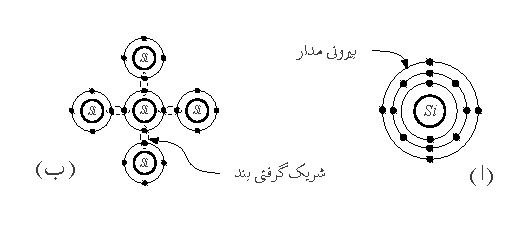
\includegraphics[scale=0.90]{covalentBond}
\caption{سلیکان ایٹم اور سلیکان قلم میں شریک گرفتی بند}
\label{شکل_سلیکان_ایٹم_اور_شریک_گرفتی_بند}
\end{figure}
حتمی صفر حرارت \عددی{\SI{0}{\kelvin}} پر موجود سلیکان کے قلم میں تمام شریک گرفتی بند برقرار رہتے ہیں اور یوں اس میں آزاد الیکٹران  کے عدم موجودگی کی وجہ سے یہ غیر موصل ہوتا ہے۔جیسے جیسے سلیکان کا درجہ حرارت بلند کیا جائے، حرارتی توانائی کی بنا پر اس میں جگہ جگہ شریک گرفتی بند منقطع ہونا شروع ہو جاتے ہیں۔

شریک گرفتی بند میں قید الیکٹران اس بند کے ٹوٹنے سے آزاد ہو جاتا ہے۔بند کے ٹوٹنے سے الیکٹران خارج ہو کر آزاد منفی چارج کے طور  سلیکان میں حرکت کرتا ہے اور یوں یہ قلم کی موصلیت میں کردار ادا کرتا ہے۔اس طرح شریک گرفتی بند کی قید سے آزاد ہوا الیکٹران جو اب سلیکان میں آزادی سے حرکت کر سکتا ہو کو \موٹا{آزاد الیکٹران}\فرہنگ{آزاد!الیکٹران}\فرہنگ{free electron}\حاشیہب{free electron} یا \موٹا{متحرک الیکٹران}\فرہنگ{متحرک الیکٹران}\فرہنگ{mobile!electron}\حاشیہب{mobile electron}  کہتے ہیں۔اسی طرح شریک گرفتی بند ٹوٹنے کی وجہ سے الیکٹران کے اخراج سے اس مقام پر \موٹا{خالی خلاء} رہ جاتا ہے اور یہاں موجود سلیکان کا ایٹم مثبت چارج اختیار کر لیتا ہے۔مثبت ایٹم قریب موجود شریک گرفتی بندوں سے الیکٹران کھنچنے کی کوشش کرتا ہے اور کبھی کبھار ایسا کرنے میں کامیاب ہو جاتا ہے۔یوں اس ایٹم کا چارج دوسرے ایٹم کو منتقل ہو جاتا ہے اور ساتھ ہی ساتھ اس خلاء کا مقام بھی تبدیل ہو کر دوسرے ایٹم کے مقام پر منتقل ہو جاتا ہے۔ایسا بار بار ہونے سے خلاء مسلسل جگہ تبدیل کرتا ہے۔خلاء اور مثبت ایٹم کا مقام ایک ساتھ حرکت کرتے ہیں گویا کہ خلاء از خود مثبت چارج ہو۔یوں سلیکان میں آزادی سے حرکت کرتے مثبت خلاء کو \موٹا{آزاد خول}\فرہنگ{آزاد!خول}\فرہنگ{free hole}\حاشیہب{free hole} یا \موٹا{متحرک خول}\فرہنگ{متحرک خول}\فرہنگ{mobile!hole}\حاشیہب{mobile hole}  کہتے ہیں۔آزاد خول بالکل \موٹا{آزاد الیکٹران} کی طرح سلیکان کی موصلیت میں کردار ادا کرتا ہے۔آزاد خول کا چارج الیکٹران کے چارج کے برابر مگر مثبت ہوتا ہے۔

حرارت سے \موٹا{شریک گرفتی بند} ٹوٹنے کی وجہ سے پیدا \موٹا{آزاد الیکٹران} (منفی چارج) کو \موٹا{حرارتی الیکٹران}\فرہنگ{حرارتی!الیکٹران}
\فرہنگ{thermal!electron}\حاشیہب{thermal electron}  جبکہ اس سے پیدا \موٹا{آزاد خول} (مثبت چارج) کو \موٹا{حرارتی خول}\فرہنگ{حرارتی!خول}
\فرہنگ{thermal!hole}\حاشیہب{thermal hole}  بھی کہتے ہیں۔چونکہ ایک شریک گرفتی بند ٹوٹنے سے ایک آزاد الیکٹران اور ایک آزاد خول وجود میں آتے ہیں لہٰذا حرارتی الیکٹران اور حرارتی خول کی تعداد ہر صورت برابر رہتی ہے۔حرارت سے پیدا الیکٹران اور خول کو \موٹا{اقلیتی الیکٹران}\فرہنگ{اقلیتی!الیکٹران}\فرہنگ{minority!electrons}\حاشیہب{minority electrons}  اور \موٹا{اقلیتی خول}\فرہنگ{اقلیتی!خول}\فرہنگ{minority!hole}\حاشیہب{minority hole}  بھی کہتے ہیں۔حرارت سے آزاد الیکٹران اور آزاد خول کے پیدائش کے عمل کو \موٹا{حرارتی پیدائش}\فرہنگ{حرارتی!پیدائش}\فرہنگ{thermal!generation}\حاشیہب{thermal generation}  کہتے ہیں۔\موٹا{حرارتی پیدائش کی شرح}\فرہنگ{حرارتی!پیدائش کی شرح}\فرہنگ{thermal!generation rate}\فرہنگ{generation rate}\حاشیہب{thermal generation rate}  کا انحصار درجہ حرارت پر ہے۔

آزاد الیکٹران اور آزاد خول سلیکان میں بلا ترتیب حرکت کرتے ہیں اور ایسا کرتے ہوئے کبھی کبھار آپس میں دوبارہ جڑ جاتے ہیں۔ان کے جڑنے سے ایک آزاد الیکٹران اور ایک آزاد خول کا وجود ختم ہو جاتا ہے۔اس عمل کو \موٹا{دوبارہ جڑنا}\فرہنگ{دوبارہ!جڑنا}\فرہنگ{جڑنا!دوبارہ}\فرہنگ{recombination}\حاشیہب{recombination}  جبکہ اس کی شرح کو \موٹا{دوبارہ جڑنے کی شرح}\فرہنگ{دوبارہ!جڑنے کی شرح}\فرہنگ{جڑنا!شرح}\فرہنگ{recombination rate}\حاشیہب{recombination rate} کہتے ہیں۔

جب حرارتی پیدائش کی شرح اور دوبارہ چڑنے کی شرح برابر ہو تو اس صورت کو \موٹا{حرارتی توازن} کہتے ہیں۔نیم موصل اشیاء کی طبیعیات سے معلوم ہوتا ہے کہ حرارتی پیدائش سے پیدا آزاد الیکٹران کی \موٹا{تعدادی کثافت}\فرہنگ{تعدادی کثافت}\فرہنگ{number density}\حاشیہب{number density} \عددی{n}  یا آزاد خول کی تعدادی کثافت  \عددی{p} کو مندرجہ ذیل مساوات سے حاصل کیا جا سکتا ہے۔
\begin{align} \label{مساوات_ڈایوڈ_حرارتی_توازن_میں_تعدادی_کثافت}
p_i^{2}=n_i^{2}=B T^{3} e^{-\frac{E_{\sigma}}{k T}}
\end{align}
جہاں
\begin{description}
\item
[\عددی{n_i} ] حرارتی الیکٹران کی تعداد فی مربع سنٹی میٹر ہے۔
\item
[\عددی{p_i}  ] حرارتی خول کی تعداد فی مربع سنٹی میٹر ہے۔
\item
[\عددی{B} ] کی مقدار ہر عنصر کے لئے مختلف ہے۔سلیکان کے لئے اس کی قیمت \عددی{\num{5.4e31}} ہے۔
\item
[\عددی{T}] حتمی حرارت ہے۔اس کی اکائی کیلون \عددی{\si{\kelvin}} ہے۔
\item
[\عددی{k} ]  بولٹزمن کا مستقل \عددی{\SI{8.62e-5}{\eV/\kelvin}}
\item
[\عددی{E_G}]  یہ شریک گرفتی بند منقطع کرنے کے لئے درکار توانائی ہے جس کی قیمت سلیکان کے لئے \عددی{ \SI{1.12}{\eV}} ہے۔
\end{description}



یاد رہے کہ حرارتی الیکٹران اور حرارتی خول کی تعدادی کثافتیں برابر ہوتی ہیں۔یعنی
\begin{align}
n_i = p_i
\end{align}

\حصہ{منفی قسم کا نیم موصل}
کیمیائی دوری جدول کے پانچویں جماعت میں نائٹروجن \عددیء{\ce{N}}، فاسفورس \عددی{\ce{P}}  وغیرہ پائے جاتے ہیں۔ان عناصر کے ایٹموں کے بیرونی مدار میں پانچ الیکٹران پائے جاتے ہیں۔نائٹروجن کو مثال بناتے دیکھتے ہیں کہ سلیکان کے قلم میں ان عناصر کی، نہایت باریک مقدار میں، موجودگی کے کیا اثرات مرتب ہوتے ہیں۔

سلیکان کے قلم میں سلیکان کے ایٹم ایک خاص ترتیب سے جڑے ہوتے ہیں۔سلیکان کے قلم میں شامل کئے جانے والے ملاوٹی نائٹروجن کے ایٹموں کی تعداد   نہایت کم ہوتی ہے اور یوں نائٹروجن کے ایٹموں کی موجودگی کا قلم میں ایٹموں کے ترتیب پر کوئی اثر نہیں ہوتا۔شامل کئے جانے والے ملاوٹی  نائٹروجن کے ایٹم قلم میں جگہ جگہ سلیکان ایٹم کی جگہ لے کر  قلم  کا حصہ بن جاتے ہیں۔شکل  \حوالہ{شکل_منفی_نیم_موصل_کا_حصول} میں نائٹروجن کے ایٹم کو سلیکان کے قلم میں بستے دکھایا گیا ہے۔نائٹروجن ایٹم کے بیرونی مدار میں موجود پانچ الیکٹرانوں میں سے چار الیکٹران قلم میں قریب چار سلیکان ایٹموں کے ساتھ شریک گرفتی بند بنانے ہیں جبکہ پانچواں الیکٹران فالتو رہ جاتا ہے۔اس فالتو الیکٹران کا نائٹروجن ایٹم کے ساتھ کمزور بند\حاشیہب{bond}  ہوتا ہے جسے الیکٹران کی حرارتی توانائی جلد منقطع کر کے الیکٹران کو آزاد کر دیتی ہے۔اس طرح آزاد الیکٹران قلم میں مکمل آزادی کے ساتھ حرکت کر سکتے ہیں جس سے قلم موصل ہو جاتا ہے۔قلم میں نائٹروجن ایٹموں کی تعداد تبدیل کر کے اس کی موصلیت پر قابو رکھا جاتا ہے۔شکل \حوالہ{شکل_منفی_نیم_موصل_کا_حصول}  میں ایک آزاد الیکٹران\حاشیہب{free electron}  کو سلیکان ایٹموں کے مابین دکھایا گیا ہے۔یوں اگر شامل کئے گئے ملاوٹی نائٹروجن ایٹموں کی تعدادی کثافت \عددی{N_D} ایٹم فی مربع سنٹی میٹر ہو تب اس سے پیدا آزاد الیکٹرانوں کی کثافت \عددی{n_{n0}} تقریباً اتنی ہی ہو گی یعنی
\begin{align}
n_{n0} \approx N_D
\end{align}
اس مساوات میں حرارتی آزاد الیکٹرانوں کی تعداد کو نظر انداز کیا گیا ہے جو کہ ایک جائز قدم ہے۔نیم موصل اشیاء کی طبیعیات سے معلوم ہوتا ہے کہ حرارتی توازن کی صورت میں آزاد الیکٹران کی کثافت \عددی{n_{n0}}  اور آزاد خول کی کثافت \عددی{p_{n0}}  کے ضرب کا جواب اٹل ہوتا ہے یعنی
\begin{align} \label{مساوات_ڈایوڈ_حرارتی_توازن_میں_اٹل_تعدادی_کثافتیں}
n_{n0} p_{n0} = n_i^{2}
\end{align}
جہاں کسی بھی درجہ حرارت پر \عددی{n_i^2} کی قیمت مساوات \حوالہ{مساوات_ڈایوڈ_حرارتی_توازن_میں_تعدادی_کثافت}  سے حاصل ہو گی۔یوں منفی نیم موصل سلیکان میں آزاد خول کی کثافت
\begin{align}
p_{n0} = \frac{n_i^2}{n_{n0}} \approx \frac{n_i^2}{N_D}
\end{align}
ہو گی۔منفی نیم موصل میں \موٹا{اکثریتی الیکٹرانوں}\فرہنگ{اکثریتی!الیکٹران}\فرہنگ{majority!electrons}\حاشیہب{majority electrons} کی کثافت شامل کئے جانے والے ملاوٹی ایٹموں کی تعداد پر منحصر ہے جبکہ اس میں \موٹا{اقلیتی خول}\حاشیہب{minority holes} کی کثافت درجہ حرارت پر منحصر ہے۔ منفی نیم موصل میں آزاد الیکٹران کی تعداد آزاد خول کی تعداد سے کئی درجہ زیادہ ہو گی۔

اس مثال میں نائٹروجن کی شمولیت سے سلیکان میں متحرک آزاد الیکٹران یعنی \موٹا{متحرک منفی چارج}\فرہنگ{متحرک منفی چارج}\حاشیہب{mobile negative charge}  نے \موٹا{موصلیت} پیدا کی۔ایسے سلیکان کو \موٹا{منفی قسم} کا نیم موصل یا \قریب{\موٹا{منفی نیم موصل}}\فرہنگ{منفی نیم موصل}\فرہنگ{نیم موصل!منفی}
\فرہنگ{n-type semiconductor}\حاشیہب{n-type semiconductor}  کہتے ہیں۔یوں منفی نیم موصل تیار کرنے کی خاطر سلیکان میں کیمیائی دوری جدول کے پانچویں جماعت کے عناصر بطور \موٹا{ملاوٹ} شامل کئے جاتے ہیں۔
\begin{figure}
\centering
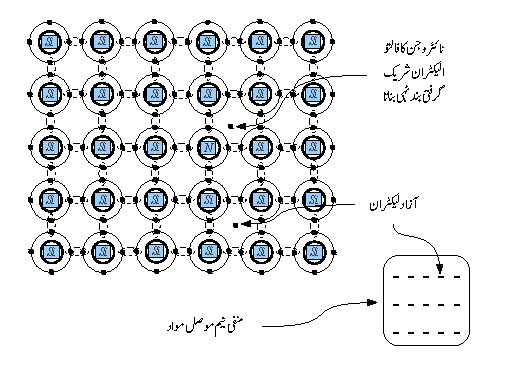
\includegraphics[scale=0.90]{nSemiconductor}
\caption{نائٹروجن کی شمولیت سے منفی قسم کے نیم موصل کا حصول}
\label{شکل_منفی_نیم_موصل_کا_حصول}
\end{figure}
کسی بھی مکمل ایٹم میں پروٹون اور الیکٹران کی تعداد برابر ہوتی ہے۔یوں ایٹم کا کُل چارج صفر ہوتا ہے۔سلیکان میں نائٹروجن بطور ملاوٹ شامل کرنے سے اس کا کُل چارج صفر ہی رہتا ہے۔نائٹروجن ایٹم کے فالتو الیکٹران کی جدائی کے بعد نائٹروجن ایٹم مثبت چارج رکھتا ہے۔یوں اگرچہ قلم کا کل چارج اب بھی صفر ہی ہے لیکن جس مقام پر نائٹروجن کا مثبت ایٹم موجود ہو اس مقام پر کل چارج مثبت ہو گا اور جس مقام پر آزاد الیکٹران موجود ہو وہاں کل چارج منفی ہو گا۔

قلم میں تمام ایٹم اپنی اپنی جگہ جکڑے رہتے ہیں۔یہ اپنی اپنی جگہ جھول سکتے ہیں لیکن جگہ تبدیل نہیں کر سکتے۔ایسے ایٹموں کو ساکن تصور کرتے ہوئے ہم دیکھتے ہیں کہ قلم میں جگہ جگہ ساکن مثبت چارج والے نائٹروجن ایٹم پائے جاتے ہیں۔یوں منفی قسم کے نیم موصل قلم میں مثبت چارج ساکن رہتے ہیں جبکہ اس میں منفی چارج (آزاد الیکٹران) حرکت پذیر ہوتے ہیں۔یوں منفی نیم موصل مواد میں برقی رو کا بہاو آزاد الیکٹران کے حرکت سے ہوتا ہے۔آزاد الیکٹران نیم موصل مواد کے وجود میں بالکل اسی طرح حرکت کرتے ہیں جیسے بند ڈبہ میں گیس کے ایٹم یا مالیکیول حرکت کرتے ہیں۔ اسی وجہ سے آزاد الیکٹران کو کبھی کبھار \موٹا{الیکٹران گیس}\فرہنگ{الیکٹران گیس}\فرہنگ{electron gas}\حاشیہب{electron gas}   بھی کہا جاتا ہے۔

ان دو اقسام کے چارجوں کا تذکرہ کرتے عموماً \موٹا{ساکن چارج}\فرہنگ{ساکن چارج}\فرہنگ{immobile!charges}\حاشیہب{immobile charges}  اور \موٹا{متحرک چارج}\فرہنگ{متحرک چارج}\فرہنگ{mobile!charges}\حاشیہب{mobile charges}  کی بات کی جاتی ہے۔یوں منفی قسم کے نیم موصل مادے میں موصلیت صرف \موٹا{متحرک چارجوں} کی وجہ سے پیدا ہوتی ہے ۔ساکن چارج کا قلم کے موصلیت پیدا کرنے  میں کوئی کردار نہیں۔منفی نیم موصل مواد کو ظاہر کرنا بھی شکل  میں دکھایا گیا ہے جہاں \عددی{(-)} آزاد الیکٹران کے وجود کو اجاگر کرتا ہے نا کہ کُل برقی چارج کو۔سلیکان میں بیرونی مادہ مثلاً نائٹروجن  کے شمولیت سے پیدا آزاد الیکٹران کو \موٹا{اکثریتی الیکٹران}\فرہنگ{اکثریتی!الیکٹران}\فرہنگ{majority!electrons}\حاشیہب{majority electrons}  بھی کہتے ہیں۔

\حصہ{مثبت قسم کا نیم موصل}
کیمیائی دوری جدول کے تیسرے جماعت میں بوران \عددیء{\ce{B}}، المونیم \عددی{\ce{Al}}  وغیرہ پائے جاتے ہیں جن کے بیرونی مدار میں صرف تین الیکٹران ہوتے ہیں۔سلیکان کے قلم میں اس جماعت کے عناصر کی شمولیت کے اثرات دیکھنے کی خاطر المونیم کی شمولیت کو مثال بناتے ہیں۔
\begin{figure}
\centering
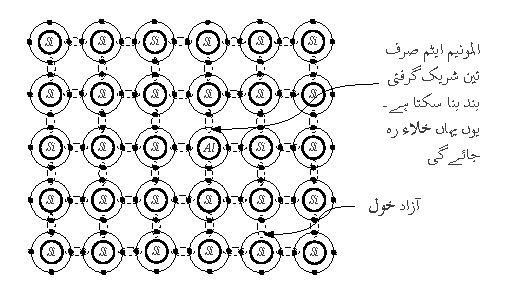
\includegraphics[scale=0.90]{pSemiconductor}
\caption{ المونیم ایٹم قلم میں سلیکان ایٹم کی جگہ لیتا ہے}
\label{شکل_مثبت_نیم_موصل}
\end{figure}
سلیکان کے قلم میں سلیکان کے ایٹم ایک خاص ترتیب سے جڑے ہوتے ہیں۔سلیکان کے قلم میں بطور ملاوٹ شامل کئے جانے والے المونیم ایٹموں کی تعداد نہایت کم ہونے کی بنا پر یہ قلم میں ایٹموں کے ترتیب پر اثر انداز نہیں ہوتے۔شامل کئے جانے والے ملاوٹی المونیم کے ایٹم قلم میں جگہ جگہ سلیکان ایٹم کی جگہ لے کر  قلم  کا حصہ بن جاتے ہیں۔

شکل \حوالہ{شکل_مثبت_نیم_موصل}  میں المونیم کے ایٹم کو سلیکان کے قلم میں بستے دکھایا گیا ہے۔قلم میں بستے المونیم ایٹم کے بیرونی مدار میں موجود تین الیکٹران قلم میں قریب تر تین سلیکان ایٹموں کے ساتھ شریک گرفتی بند بنا لیتے ہیں۔المونیم ایٹم کے بیرونی مدار میں چوتھے الیکٹران کی عدم موجودگی کی بنا پر قریب چوتھے سلیکان ایٹم کے ساتھ شریک گرفتی بند بنانا ممکن نہیں ہوتا۔یوں اس بند کی جگہ خلاء رہ جاتی ہے۔

شکل \حوالہ{شکل_آزاد_خول}  کو دیکھتے ہوئے آگے پڑھیں۔حرارتی توانائی سے عین ممکن ہوتا ہے کہ اس خلاء کے قریب کوئی شریک گرفتی بند منقطع ہو جائے اور وہاں سے الیکٹران خارج ہو جائے۔ خارج شدہ الیکٹران بھٹکتا بھٹکتا المونیم کے قریب خلاء کو پُر کر کے  یہاں شریک گرفتی بند کو جنم دیتا ہے۔ایسا ہونے سے المونیم ایٹم منفی چارج اختیار کر لیتا ہے جبکہ جہاں سے الیکٹران خارج ہوا ہو اس مقام پر مثبت \موٹا{آزاد خول}\فرہنگ{آزاد!خول}\فرہنگ{free hole}\حاشیہب{free hole}  رہ جاتا ہے۔اس مثبت آزاد خول کو خول  الف کہتے ہوئے گفتگو آگے بڑھاتے ہیں۔اسی طرح حرارتی توانائی نو پیدا خول  الف کے قریب کسی اور شریک گرفتی بند کو منقطع کر کے یہاں سے الیکٹران خارج کرتے ہوئے خول  ب پیدا کرے گا اور خارج الیکٹران خول  الف تک پہنچ کر اسے پُر کر کے یہاں خول کے وجود کو ختم کر دے گا۔اسی طرح خول  پ پیدا ہونے سے خول  ب پُر ہو گا وغیرہ وغیرہ۔یوں آزاد خول مسلسل جگہ تبدیل کرے گا جبکہ منفی المونیم ایٹم ساکن رہتا ہے۔مسلسل حرکت پذیر مثبت خول  (آزاد خول) کی بدولت قلم کی موصلیت وجود میں آتی ہے جبکہ ساکن منفی چارج (المونیم ایٹم) کا قلم کی موصلیت میں کوئی کردار نہیں۔یوں مثبت نیم موصل مواد میں برقی رو کا بہاو آزاد خول کے حرکت سے ہوتا ہے۔ 

چونکہ اس طرح کے قلم میں خول 	بطور مثبت چارج کردار ادا کرتا ہے اور یہی موصلیت کو جنم دیتا ہے لہٰذا اسے \موٹا{مثبت قسم} کی نیم موصل مواد یا \موٹا{مثبت نیم موصل}\فرہنگ{مثبت نیم موصل}\فرہنگ{نیم موصل!مثبت}\فرہنگ{p-type semiconductor}\حاشیہب{p-type semiconductor}  کہتے ہیں۔مثبت نیم موصل مواد کو ظاہر کرنا بھی شکل \حوالہ{شکل_آزاد_خول}  میں دکھایا گیا ہے جہاں \عددی{(+)} آزاد خول کے وجود کو اجاگر کرتا ہے نا کہ کُل برقی چارج کو۔

اس طرح آزاد خول قلم میں مکمل آزادی کے ساتھ حرکت کر سکتے ہیں جس سے قلم موصل ہو جاتا ہے۔قلم میں المونیم ایٹموں کی تعداد تبدیل کر کے اس کی موصلیت پر قابو رکھا جاتا ہے۔آزاد خول  نیم موصل مواد کے وجود میں بالکل اسی طرح حرکت کرتے ہیں جیسے بند ڈبہ میں گیس کے ایٹم یا مالیکیول حرکت کرتے ہیں۔ اسی وجہ سے آزاد خول کو کبھی کبھار \موٹا{خول گیس}\فرہنگ{خول گیس}\فرہنگ{hole gas}\حاشیہب{hole gas}   بھی کہا جاتا ہے۔سلیکان میں بیرونی مواد مثلاً \عددی{\ce{Al}} کے شمولیت سے پیدا آزاد خول کو \موٹا{اکثریتی خول}\فرہنگ{اکثریتی!خول}\فرہنگ{majority!holes}\حاشیہب{majority holes}  بھی کہتے ہیں۔
\begin{figure}
\centering
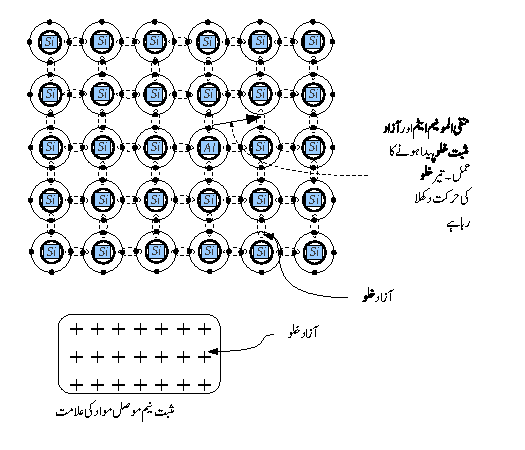
\includegraphics[scale=0.90]{freeHoles}
\caption{ آزاد خول کی حرکت اور مثبت نیم موصل مواد ظاہر کرنے کی علامت}
\label{شکل_آزاد_خول}
\end{figure}
مثبت نیم موصل سلیکان بناتے وقت اگر اس میں شامل کئے جانے والے ملاوٹی ایٹموں کی کثافت \عددی{N_A} ایٹم فی مربع سینٹی میٹر ہو تب اس میں حرارتی آزاد خول کو نظر انداز کرتے ہوئے اکثریتی آزاد خول کی کثافت \عددی{p_{n0}} بھی تقریباً اتنی ہو گی یعنی
\begin{align}
p_{p0}=N_A
\end{align}
جبکہ حرارتی متوازن صورت میں اس میں آزاد الیکٹرانوں کی کثافت مساوات \حوالہ{مساوات_ڈایوڈ_حرارتی_توازن_میں_اٹل_تعدادی_کثافتیں}  کے تحت
\begin{align}
n_{p0}=\frac{n_i^2}{p_{p0}} \approx \frac{n_i^2}{N_A}
\end{align}
ہو گا۔مثبت نیم موصل میں اکثریتی خول\حاشیہب{majority holes} کی کثافت شامل کئے جانے والے ملاوٹی  ایٹموں کی تعداد پر منحصر ہے جبکہ اس میں اقلیتی الیکٹرانوں\حاشیہب{minority electrons} کی کثافت درجہ حرارت پر منحصر ہے۔
\حصہ{مال برداری}
 آزاد الیکٹران اور آزاد خول \موٹا{نفوذ}\فرہنگ{نفوذ}\فرہنگ{diffusion}\حاشیہب{diffusion}  اور \موٹا{بہاو}\فرہنگ{بہاو}\فرہنگ{drift}\حاشیہب{drift}  کے ذریعہ سلیکان میں حرکت کر کے ایک مقام سے دوسرے مقام منتقل ہو سکتے ہیں۔کائنات میں قدرتی \موٹا{مال برداری}\فرہنگ{مال برداری}\فرہنگ{transportation}\حاشیہب{transportation}  ان دو خود کار طریقوں سے ہوتی ہے۔پانی میں سیاہی کا پھیلاو اور دریا میں پانی کا بہاو انہیں کی بدولت ہے۔

\جزوحصہ{نفوذ} 
نفوذ سے مراد الیکٹران اور خول کی وہ بلا ترتیب حرکت ہے جو حرارتی توانائی کی وجہ سے پیدا ہوتی ہے۔سلیکان میں آزاد الیکٹران (آزاد خول) کی یکساں تعدادی کثافت کی صورت میں آزاد الیکٹران (آزاد خول)  کے نفوذ سے برقی رو پیدا نہیں ہوتی البتہ اگر کسی طرح آزاد الیکٹران (یا آزاد خول) کی تعدادی کثافت ایک مقام پر زیادہ کر دی جائے تو اس صورت میں زیادہ تعدادی کثافت والے مقام سے کم تعدادی کثافت کے مقام کی جانب آزاد الیکٹرانوں (خولوں) کا بہاو ہو گا جس سے برقی رو پیدا ہو گی۔ایسے برقی رو کو \موٹا{نفوذی برقی رو}\فرہنگ{نفوذی برقی رو}\فرہنگ{diffusion current}\حاشیہب{diffusion current}  کہتے ہیں۔اس حقیقت کو شکل \حوالہ{شکل_نفوذ}  کی مدد سے بہتر سمجھا جا سکتا ہے جہاں فرضی سلیکان کے ایک سلاخ میں لمبائی کے جانب آزاد الیکٹرانوں کی تعداد تبدیل ہوتے دکھائی گئی ہے۔اسی شکل میں اس کا گراف بھی دکھایا گیا ہے۔اس شکل میں آزاد الیکٹران دائیں جانب نفوذ کریں گے۔اس طرح سلاخ میں روایتی برقی رو کی سمت بائیں جانب ہو گی۔

پانی میں رنگ نفوذ کے ذریعہ حل ہوتا ہے۔
\begin{figure}
\centering
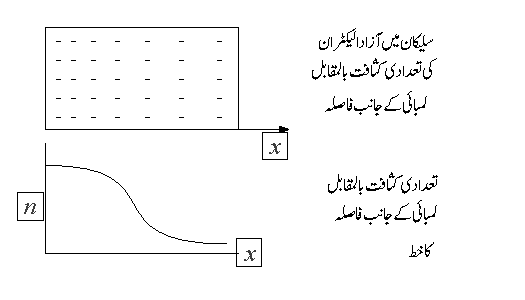
\includegraphics[scale=0.90]{diffusionCause}
\caption{ تعدادی کثافت میں نا ہمواری نفوذ پیدا کرتا ہے}
\label{شکل_نفوذ}
\end{figure}
آزاد خول کے نفوذی برقی رو کی مساوات شکل \حوالہ{شکل_آزاد_خول_سے_حاصل_برقی_رو}  کی مدد سے حاصل کرتے ہیں۔شکل میں سلیکان کی مثبت نیم موصل سلاخ دکھائی گئی ہے جس کا رقبہ عمودی تراش \عددی{A} ہے۔شکل میں نقطہ  الف پر آزاد خولوں کی تعدادی کثافت \عددی{(p)}  جبکہ اس کے قریب \عددی{\Delta x}  فاصلہ پر نقطہ  ب پر تعدادی کثافت \عددی{p+\Delta p} ہے۔ان دو نقطوں پر سلاخ کے چھوٹی سی لمبائی \عددی{\Delta x} میں کل خولوں کی تعداد \عددی{p A \Delta x}  اور \عددی{(p+\Delta p) A \Delta x} ہو گی۔ہم تصور کرتے ہیں کہ سلاخ میں خول صرف لمبائی کے جانب حرکت کرتے ہیں۔اس طرح حصہ  الف کے آدھے خول، یعنی \عددیء{p A \Delta x/2}،  بائیں جانب اور آدھے دائیں جانب حرکت کریں گے۔اسی طرح حصہ  ب کے آدھے خول، یعنی \عددی{(p+\Delta p) A \Delta x /2} ، بائیں اور آدھے دائیں جانب حرکت کریں گے۔یوں ان دو نقطوں کے درمیان نقطہ دار لکیر پر دائیں جانب گزرتے کل خولوں کی تعداد
\begin{align*}
\frac{p A \Delta x}{2}-\frac{(p+\Delta p ) A \Delta x}{2}=-\frac{\Delta p A \Delta x}{2}
\end{align*}
 ہو گی۔خول کے چارج کو \عددی{q} لکھتے ہوئے اس لکیر سے دائیں جانب گزرتے کل چارج کی مقدار کو یوں لکھا جا سکتا ہے۔
\begin{align*}
\Delta Q_p = -\frac{q \Delta p A \Delta x}{2}
\end{align*}
	تصور کریں کہ چارجوں کی یوں منتقلی وقت \عددی{\Delta t}  میں عمل میں آتی ہے۔اس طرح سلاخ میں برقی رو \عددی{I_p = \Delta Q_p / \Delta t}ہو گی یعنی
\begin{align*}
I_p=\frac{\Delta Q_p}{\Delta t} = -\frac{q \Delta p A \Delta x}{2 \Delta t}
\end{align*}
اس برقی رو کی کثافت \عددی{J_p} کو یوں لکھا جا سکتا ہے۔
\begin{align}
J_p=\frac{I_p}{A} = -\frac{q \Delta p \Delta x}{2 \Delta t}
\end{align}
کسی بھی تفاعل \عددی{y}  کے لئے ہم لکھ سکتے ہیں
 \عددی{\Delta y =\od{y}{x} \Delta x}
یوں موجودہ صورت میں لکھا جا سکتا ہے۔
\begin{align}
\Delta p = \od{p}{x} \Delta x
\end{align}
ان دو مساواتوں سے حاصل ہوتا ہے
\begin{align}
J_p = \frac{I_p}{A}=-q \od{p}{x} \frac{\Delta x^2}{2 \Delta t}
\end{align}
اس مساوات میں
\begin{align}
D_p = \frac{\Delta x^2}{2 \Delta t}
\end{align}
لکھ کر حاصل ہوتا ہے
\begin{align}
J_p = -q D_p \od{p}{x}
\end{align}
یہ مساوات نفوذی برقی رو کی کثافت یا \موٹا{کثافتِ نفوذی رو}\فرہنگ{کثافتِ نفوذی رو}\فرہنگ{diffusion current density}\حاشیہب{diffusion current density} کو بیان کرتا ہے۔\حاشیہد{نفوذ کے ذریعہ مال برداری کے اس قلیہ کو اڈلف فِق Adolf Fick نے دریافت کیا}
\begin{figure}
\centering
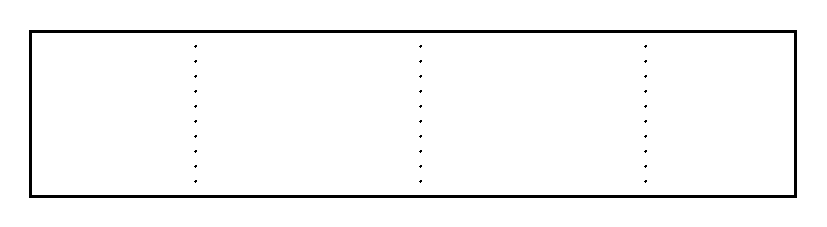
\includegraphics[scale=0.90]{diffusionCurrent}
\caption{  آزاد خول سے حاصل نفوذی برقی رو}
\label{شکل_آزاد_خول_سے_حاصل_برقی_رو}
\end{figure}
جہاں
\begin{description}
\item
[\عددی{J_p} ] آزاد خولوں سے پیدا نفوذی برقی رو کی کثافت\حاشیہب{diffusion current density}  ہے۔
\item
[\عددی{q}] خول کے چارج کی مقدار یعنی \عددی{\SI{1.6e-19}{\coulomb}} ہے۔
\item
[\عددی{D_p}] خول کے \موٹا{نفوذ کا مستقل}\فرہنگ{نفوذ کا مستقل!خول}\فرہنگ{مستقل!نفوذِ خول}\فرہنگ{diffusion constant! holes}\حاشیہب{hole's diffusion constant}  ہے۔سلیکان میں \عددی{D_p =\SI{12}{cm^2 /s}}کے برابر ہوتا ہے۔
\item
[\عددی{p}] آزاد خول کی تعدادی کثافت ہے۔
\end{description}


آزاد الیکٹرانوں کے لئے نفوذی برقی رو کی کثافت کی مساوات مندرجہ ذیل ہے۔
\begin{align}
J_n = q D_n \od{n}{x}
\end{align}
اس مساوات میں منفی کی علامت استعمال نہ کرنے سے ہی برقی رو کی صحیح سمت حاصل ہوتی ہے۔ \عددی{D_n} آزاد الیکٹران کے \موٹا{نفوذ کا مستقل}\فرہنگ{نفوذ کا مستقل!الیکٹران}\فرہنگ{مستقل!نفوذِ الیکٹران}\فرہنگ{diffusion constant! electrons}\حاشیہب{electron's diffusion constant} ہے جس کی قیمت سلیکان کے لئے \عددی{\SI{34}{cm^2/s}} ہے۔

\جزوحصہ{بہاو}
	آزاد الیکٹران اور آزاد خول کے حرکت کرنے کا دوسرا ذریعہ \موٹا{بہاو}\فرہنگ{بہاو}\فرہنگ{drift}\حاشیہب{drift} ہے ۔بہاو سے پیدا برقی رو کو \موٹا{بہاو برقی رو}\فرہنگ{بہاو برقی رو}\فرہنگ{drift current}\حاشیہب{drift current}  کہتے ہیں۔

اگر سلیکان کے ایک سلاخ، جس کی لمبائی \عددی{L} ہو، کے دو سروں کے مابین برقی دباو \عددی{V} مہیا کی جائے تو اس سلاخ میں \موٹا{برقی!شدت}\فرہنگ{برقی شدت}\فرہنگ{electric field intensity}\حاشیہب{electric field intensity}  \عددی{E} پیدا ہو گی جہاں
\begin{align*}
E=\frac{V}{L}
\end{align*}
کے برابر ہے۔برقی دباو کی شدت آزاد الیکٹران اور آزاد خول کو اسراع دے گا۔آزاد خول کا رفتار برقی شدت کی سمت میں جبکہ آزاد الیکٹران کا رفتار اس کے اُلٹ سمت میں بڑھے گا۔برقی شدت سے پیدا چارجوں کے رفتار کو \موٹا{رفتارِ بہاو}\فرہنگ{رفتار بہاو}\فرہنگ{drift speed}\حاشیہب{drift speed}  کہتے ہیں۔آگے صرف آزاد الیکٹران پر گفتگو کرتے ہیں اگرچہ  یہ سب کچھ آزاد خول کے لئے بھی درست ہے۔اس گفتگو میں آزاد الیکٹران کو صرف الیکٹران کہیں گے۔

الیکٹران کی رفتار کے دو اجزاء ہیں۔ایک جزو حرارتی رفتار ہے جبکہ دوسرا جزو بہاو کی رفتار یا رفتارِ بہاو ہے۔اگر سلیکان کے سلاخ میں ہر مقام پر حرارت یکساں ہو تب اس سلاخ میں حرارتی رفتار کی اوسط قیمت ہر مقام پر برابر ہو گی۔حرارتی رفتار بلا ترتیب ہے اور یوں سمتی حرارتی رفتار کی اوسط قیمت صفر ہوتی ہے۔لہٰذا اس صورت میں سمتی حرارتی رفتار کا سلیکان میں برقی رو پیدا کرنے میں کوئی کردار نہیں۔اس کے برعکس الیکٹران کی \موٹا{سمتی رفتارِ بہاو}\فرہنگ{سمتی رفتارِ بہاو}\فرہنگ{drift velocity}\حاشیہب{drift velocity}  برقی شدت کے اُلٹ سمت میں ہوتی ہے اور اس کی اوسط قیمت برقی شدت پر منحصر ہوتی ہے۔یوں برقی شدت کے موجودگی میں سلیکان میں برقی رو سمتی رفتارِ بہاو کے وجہ سے ہوتی ہے۔سمتی رفتارِ بہاو پر اب گفتگو کرتے ہیں۔

برقی شدت کی وجہ سے حرکت کرتے چارج وقتاً فوقتاً ساکن ایٹموں کے ساتھ ٹکرا کر اپنی توانائی ضائع کر دیتے ہیں اور ان کی \موٹا{لمحاتی سمتی رفتارِ بہاو}\حاشیہب{instantaneous drift velocity}  صفر ہو جاتی ہے۔ٹکرانے کے بعد یہ ایک بار پھر برقی شدت کی وجہ سے رفتار پکڑتے ہیں۔یوں ٹکرانے کی وجہ سے الیکٹران کی رفتار لگاتار نہیں بڑھتی بلکہ یہ کسی اوسط رفتار سے سلیکان میں برقی شدت کے اُلٹ سمت حرکت کرتے ہیں۔اس اوسط سمتی رفتار کو \موٹا{اوسط سمتی رفتارِ بہاو}  یا صرف \موٹا{سمتی رفتارِ بہاو} کہتے ہیں۔ 

سلیکان کے قلم میں برقی شدت \عددی{E} کے موجودگی میں الیکٹران پر قوت \عددی{F=-q E} عمل کرے گا۔اس قوت کی وجہ سے الیکٹران اسراع \عددی{a}  پکڑے گا جسے \موٹا{نیوٹن}\حاشیہب{Newton' law} کے مساوات \عددی{F=m_n a}  سے حاصل کیا جا سکتا ہے یعنی
\begin{align*}
a=-\frac{q E}{m_n}
\end{align*}
اگر الیکٹران کے ٹکرانے کا اوسط وقفہ  \عددی{t_n} ہو تو اتنے وقت میں ساکن حال سے چلا الیکٹران رفتار \عددی{v_{t_n}} اختیار کرے گا جہاں
\begin{align*}
v_{t_n}= a \times t_n = -\frac{q E t_n}{m_n}
\end{align*}
دورانیہ \عددی{t_n} میں یوں الیکٹران کا اوسط رفتار اس کے آدھا ہو گا یعنی
\begin{align*}
v_n =\frac{v_{t_n}}{2}=-\frac{q E t_n}{2 m_n}
\end{align*}
اس مساوات میں \عددی{\mu_n = \frac{q t_n}{2 m_n}} لکھنے سے اسے یوں لکھا جا سکتا ہے
\begin{align}
v_n = -\mu_n E
\end{align}
جہاں  \عددی{\mu_n} کو الیکٹران کی \موٹا{حرکت پذیری}\فرہنگ{حرکت پذیری!الیکٹران}\فرہنگ{electron mobility}\حاشیہب{electron mobility} کہتے ہیں۔اگر سمتی رفتارِ بہاو کو\عددی{\si{cm/s}}  اور برقی شدت کو \عددی{\si{V/cm}} میں ناپا جائے تو سلیکان میں الیکٹران کی \موٹا{حرکت پذیری} \عددی{\mu_n} کی قیمت \عددی{\SI{1350}{cm^2/Vs}}\شناخت{الیکٹران_کی_حرکت_پذیری} ہے۔اسی طرح آزاد خول کے لئے ہم لکھ سکتے ہیں۔
\begin{align}
v_p = \mu_p E
\end{align}
جہاں سلیکان میں آزاد خول کی حرکت پذیری \عددی{\mu_p} کی قیمت \عددی{\SI{480}{cm^2/Vs}} کے لگ بھگ ہے۔سلیکان کے سطح پر حرکت پذیری کی قیمت گہرائی پر حرکت پذیری کے قیمت سے دس گنا تک کم ہو سکتی ہے۔یہاں \موٹا{گہرائی پر الیکٹران کی حرکت پذیری} اور \موٹا{گہرائی پر خول کی حرکت پذیری} کی بات کی گئی۔
\begin{figure}
\centering
\includegraphics[scale=0.90]{driftCurrent}
\caption{ برقی شدت سے برقی رو کا پیدا ہونا}
\label{شکل_برقی_شدت_سے_پیدا_برقی_رو}
\end{figure}
شکل \حوالہ{شکل_برقی_شدت_سے_پیدا_برقی_رو}  میں مثبت نیم موصل سلیکان کا سلاخ دکھایا گیا ہے جس میں آزاد خول کی تعدادی کثافت \عددی{p}  فی مربع سنٹی میٹر ہے۔اگر اس سلاخ میں برقی شدت \عددی{E} ہو تو اس میں آزاد خول کی سمتی رفتارِ بہاو \عددی{v_p} اسی سمت میں ہو گی۔یوں ایک سیکنڈ میں آزاد خول اس سلاخ میں \عددی{v_p} سنٹی میٹر کا فاصلہ طے کریں گے۔سلاخ کے لمبائی \عددی{L} کا حجم \عددی{A \times L} ہے اور اتنے حجم میں \عددی{p \times A \times L}  آزاد خول ہوں گے۔یوں اتنے حجم میں کل آزاد چارج \عددی{\Delta Q=q p A L}  ہو گا۔اگر \عددی{v_p} سنٹی میٹر لمبائی کی بات کریں تو اتنے سلاخ میں موجود آزاد خول کا چارج \عددی{\Delta Q = q p A v_p} ہو گا۔سلاخ کے دائیں جانب سطح \عددی{A}  سے یوں ہر سیکنڈ \عددی{q p A v_p} چارج گزرے گا اور یوں اس سلاخ میں برقی رو \عددی{I_p} کی قیمت \عددی{q p A v_p} ہو گی۔اس برقی رو کی کثافت \عددی{J_p}
\begin{align}
J_p = \frac{I_p}{A}=q p v_p = q p \mu_p E
\end{align}
ہو گا۔

بالکل اسی طرح آزاد الیکٹران کے لئے بھی مساوات لکھی جا سکتی ہے۔آزاد الیکٹران کے چارج کو \عددی{(-q)} لکھتے ہوئے چونکہ اس کے لئے \عددی{v_n =\mu_n E} ہے لہٰذا آزاد الیکٹران کے لئے اس مساوات کو یوں لکھا جا سکتا ہے۔
\begin{align}
J_n = \frac{I_n}{A}=(-q) n v_n = (-q) n (-\mu_n) E = q n \mu_n E
\end{align}
	آزاد الیکٹران اور آزاد خول کے موجودگی میں برقی رو دونوں چارجوں کی وجہ سے پیدا ہو گی اور یوں اس صورت میں ہم لکھ سکتے ہیں۔
\begin{align}
J_\sigma=q n \mu_n E+ q p \mu_p E=q (n \mu_n+p \mu_p)E
\end{align}
اس مساوات میں  
\begin{align}
\sigma = (n \mu_n+p \mu_p)
\end{align}
لکھنے سے اسے یوں لکھا جا سکتا ہے۔
\begin{align} \label{مساوات_ڈایوڈ_اہم_کا_قانون_الف}
J_\sigma = q \sigma E
\end{align}
یہ مساوات برقی شدت کی بدولت بہاو سے پیدا برقی رو کی مساوات ہے جس میں\عددی{\sigma} سلیکان کے \موٹا{موصلیت کا مستقل}\فرہنگ{موصلیت!مستقل}\فرہنگ{conductivity}\حاشیہب{conductivity}  ہے۔مساوات \حوالہ{مساوات_ڈایوڈ_اہم_کا_قانون_الف}  درحقیقت \موٹا{قانونِ اُوہم}\حاشیہب{Ohm' law'}  ہے۔


\حصہ{مثبت اور منفی اقسام کے نیم موصل مواد کا ملاپ} 
	مثبت نیم موصل مواد اور منفی نیم موصل مواد کے ملاپ سے ڈایوڈ   وجود میں آتا ہے۔شکل \حوالہ{شکل_ڈایوڈ_کی_بناوٹ}  میں اس کی بناوٹ اور علامت دکھائی گئی ہے۔حقیقت میں ڈایوڈ تیار کرتے وقت سلیکان کی ایک ہی پتری پر منفی اور مثبت  قسم کے نیم موصل احاطے ملا کر بنائے جاتے ہیں۔
\begin{figure}
\centering
\includegraphics[scale=0.90]{pnJunctionAsDiode}
\caption{ڈایوڈ کی بناوٹ اور اس کی علامت}
\label{شکل_ڈایوڈ_کی_بناوٹ}
\end{figure}
	تصور کریں کہ مثبت نیم موصل اور منفی نیم موصل سلیکان کو جوڑا جاتا ہے۔اس وقت کا صورتِ حال شکل \حوالہ{شکل_رکاوٹی_برقی_دباو}-ا میں دکھایا گیا ہے۔نفوذ کی وجہ سے مثبت نیم موصل حصے سے آزاد خول منفی نیم موصل حصے کی جانب حرکت کریں گے اور اسی طرح منفی نیم موصل حصے سے آزاد الیکٹران مثبت نیم موصل حصے کی جانب حرکت کریں گے۔مثبت نیم موصل حصے سے خولوں کے نکل جانے سے یہاں سرحد کے قریب ساکن منفی ایٹم نمودار یا بے پردہ  ہوں گے۔اسی طرح منفی نیم موصل حصے سے الیکٹران کے نکل جانے سے یہاں سرحد کے قریب ساکن مثبت ایٹم نمودار یا بے پردہ ہوں گے۔مثبت نیم موصل حصے میں داخل الیکٹرانوں میں سے چند سرحد کے قریب آزاد خولوں سے مل کر ختم ہو جائیں گے جبکہ بقایا اس حصے میں بطور اقلیتی چارج اس وقت تک بسیں گے جب تک یہ کسی خول کے ساتھ مل کر ختم نہ ہو جائیں۔اسی طرح منفی حصے میں داخل آزاد خولوں میں سے جند یہاں آزاد الیکٹرانوں سے مل کر ختم ہو جائیں گے جبکہ بقایا اس حصے میں بطور اقلیتی چارج اس وقت تک بسیں گے جب تک یہ کسی آزاد خول کے ساتھ مل کر ختم نہ ہو جائیں۔یہ صورتِ حال شکل \حوالہ{شکل_رکاوٹی_برقی_دباو} ب میں دکھائی گئی ہے جہاں ساکن ایٹموں کو گول دائرے میں بند دکھایا گیا ہے۔آزاد الیکٹرانوں اور آزاد خولوں کے اس حرکت سے پیدا نفوذی برقی رو کو \عددی{I_D} لکھتے ہیں جہاں نیچے کر کے نفوذ کے مستقل \عددی{D} لکھنے سے اس برقی رو کی بطور نفوذی برقی رو پہچان کی گئی ہے۔
\begin{figure}
\centering
\includegraphics[scale=0.90]{diodeVoltage}
\caption{رکاوٹی برقی دباو}
\label{شکل_رکاوٹی_برقی_دباو}
\end{figure}
نیم موصل سلیکان از خود \موٹا{غیر چارج شدہ}\حاشیہب{neutral} ہوتا ہے۔شکل  ب کے دونوں جانب غیر چارج شدہ  نیم موصل سلیکان ہے جبکہ ان کے درمیانی سرحد پر چارج شدہ ساکن ایٹم نمودار ہو چکے ہیں۔اس درمیانے خطے کو \موٹا{ویران خطہ}\حاشیہب{depletion region} کہتے ہیں۔یوں سرحد کے دائیں جانب مثبت ایٹم جبکہ اس کے بائیں جانب منفی ایٹم موجود ہیں۔آپ جانتے ہیں کہ ایک جانب مثبت چارج اور دوسرے جانب منفی چارج کا وجود \موٹا{برقی شدت}\حاشیہب{electric field intensity} \عددی{E}  پیدا کرتا ہے اور ان  کے مابین برقی دباو\حاشیہب{voltage} \عددی{V_0}  پایا جاتا ہے۔یوں ویران خطے میں برقی شدت \عددی{E} پایا جائے گا۔

اگر منفی نیم موصل حصے سے حرارتی توانائی کی بدولت حرکت کرتا آزاد  خول\حاشیہد{یاد رہے کہ نیم موصل سلیکان میں حرارتی توانائی کی بدولت ہر وقت حرارتی چارج پیدا ہوتے رہتے ہیں۔} بھٹکتا ہوا ویران خطے میں داخل ہو جائے تو اس پر برقی شدت کی وجہ سے برقی قوت \عددی{F= qE}  عمل کرے گی جو اسے مثبت نیم موصل حصے میں دھکیل دے گی۔اسی طرح اگر مثبت نیم موصل حصے سے آزاد خول ویران خطے میں داخل ہو جائے تو اسے بھی مثبت نیم موصل حصے میں دھکیل دیا جاتا ہے۔ 

اگر مثبت نیم موصل حصے سے آزاد الیکٹران حرارتی توانائی کی بدولت حرکت کرتا ویران خطے پہنچ جائے تو اس پر برقی قوت \عددی{F=-q E}  عمل کر کے اسے منفی نیم موصل حصے میں دھکیل دے گی۔اسی طرح اگر منفی نیم موصل حصے سے آزاد الیکٹران ویران خطے میں داخل ہو جائے تو اسے بھی منفی نیم موصل حصے میں دھکیل دیا جاتا ہے۔ 

آپ دیکھ سکتے ہیں کہ یہ برقی شدت سے پیدا بہاو کا عمل ہے۔اس عمل سے پیدا برقی رو \عددی{I_S} کو شکل میں دکھایا گیا ہے۔چونکہ اس خطے میں کسی قسم کا آزاد چارج زیادہ دیر نہیں ٹھر سکتا اس لئے اسے \موٹا{ویران خطہ}\فرہنگ{ویران خطہ}\فرہنگ{depletion region}\حاشیہب{depletion region} کہتے ہیں۔

برقی رو \عددی{ِِI_S} کی مقدار کا دارومدار حرارتی توانائی سے حرکت کرتے اُن آزاد الیکٹرانوں اور آزاد خولوں پر ہے جو ویران خطے میں بھٹک جائیں۔اس کے برعکس برقی رو \عددی{I_D} کی مقدار دونوں نیم موصل خطوں میں شامل کئے گئے ملاوٹی ایٹموں کی تعدادی کثافت اور رکاوٹی برقی دباو \عددی{V_0} پر ہے۔یوں \عددی{I_D} کی مقدار \عددی{V_0} بڑھنے سے کم ہوتی ہے۔

جس لمحہ مثبت اور منفی نیم موصل سلیکان کو آپس میں جوڑا جائے اس لمحہ\حاشیہد{ابھی ویران خطہ پیدا نہیں ہوا ہوتا لہٰذا \عددی{I_S} صفر ہوتا ہے} صرف \عددی{I_D} برقی رو پائی جائے گی۔جیسے جیسے ویران خطے کے حدود بڑھیں گے ویسے ویسے  \عددی{E}  اور \عددی{V_0} کی مقداریں بڑھیں گے اور یوں \عددی{I_D} کی مقدار گھٹے گی جبکہ \عددی{I_S} کی مقدار بڑھے\حاشیہد{\عددی{I_S} کی قیمت حرارتی توانائی سے حرکت کرتے آزاد چارجوں کے ویران خطے میں بھٹکنے پر منحصر ہے۔ویران خطے کے حدود بڑھنے سے ایسا ہونے کے امکانات بڑھ جاتے ہیں۔} گی۔آخر کار ان دو قسموں کی برقی رو کی مقداریں برابر ہو جائیں گی (یعنی \عددی{I_D=I_S} )  اور نیم موصل جڑوا سلیکان متوازن صورت اختیار کر لے گا۔

متوازن صورتِ حال کے حصول کے بعد اگر کسی وجہ سے \عددی{I_D} کی قیمت بڑھ جائے تو اس سے مزید چارج شدہ ایٹم نمودار ہوں گے جس سے \عددی{E} اور \عددی{V_0} کی قیمت میں اضافہ ہو گا جس سے \عددی{I_D}  کے اضافے کی روک تھام ہو گی اور ایک مرتبہ دوبارہ متوازن صورتِ حال پیدا ہو گا۔اس کے برعکس اگر کسی وجہ سے  \عددی{I_D} کی قیمت میں کمی آئے تو چونکہ  \عددی{I_S} مسلسل چالو\حاشیہد{عام حالت میں ویران خطے کے حدود نہایت کم تبدیل ہوتے ہیں لہٰذا \عددی{I_S} کی قیمت کو غیر تغیر پذیر یعنی اٹل تصور کیا جاتا سکتا ہے۔} رہتا ہے لہٰذا چارج شدہ ایٹموں کی تعداد میں کمی آئے گی جس سے  \عددی{E} اور \عددی{V_0} کی قیمتوں میں کمی آئے گی۔رکاوٹی دباو میں کمی  \عددی{I_D} کے گھٹنے کو روکے گی اور ایک مرتبہ دوبارہ متوازن صورتِ حال پیدا ہو گا۔

شکل میں دکھایا برقی دباو \عددی{V_0} نفوذ کے عمل کو روکتا ہے۔اسی لئے اسے \موٹا{رکاوٹی برقی دباو}\فرہنگ{رکاوٹی برقی دباو}\فرہنگ{برقی دباو!رکاوٹی}\فرہنگ{blocking voltage}\حاشیہب{blocking voltage}  کہتے ہیں۔سلیکان میں \موٹا{رکاوٹی برقی دباو} کی عمومی  قیمت \عددی{\SI{0.6}{\volt}} تا \عددی{\SI{0.8}{\volt}} رہتی ہے۔اس کی اوسطاً قیمت کو عموماً \عددی{\SI{0.7}{\volt}} لیا جاتا ہے۔

%==========
\ابتدا{مثال}
اگر ڈایوڈ کے سروں کے مابین برقی تار جوڑی جائے تو کیا رکاوٹی برقی دباو کی وجہ سے برقی تار میں برقی رو پیدا ہو گی؟
حل:	ہرگز نہیں۔اگر ایسا ممکن ہوتا تو ہم ڈایوڈ سے لگاتار توانائی حاصل کر سکتے ہوتے جو کہ قانون برائے بقائے توانائی کے خلاف ہے۔

\انتہا{مثال}
%========

حقیقت میں ڈایوڈ کے سروں پر نیم موصل اور دھاتی برقی تار کے جوڑ  پر برقی دباو پیدا ہوتا ہے جو رکاوٹی برقی دباو کے عین برابر اور اس کے اُلٹ جانب ہوتا ہے۔اس طرح بیرونی برقی تار میں برقی رو نہیں پیدا ہوتی۔نیم موصل اور برقی تار کے جوڑ پر پیدا برقی دباو ان کے آپس میں چھونے سے پیدا ہوتا ہے۔ 	

%=======
\ابتدا{مثال}
رکاوٹی برقی دباو \عددی{V_0} کو وولٹ میٹر\حاشیہب{volt meter}  سے کیسے ناپا جاتا ہے۔
حل:	رکاوٹی برقی دباو کو وولٹ میٹر سے ناپنا ممکن نہیں۔رکاوٹی برقی دباو ناپتے وقت جیسے ہی میٹر کی برقی تاریں ڈایوڈ کے سروں کو چھوتے ہیں، ان سروں پر  برقی دباو پیدا ہوتا ہے جو رکاوٹی برقی دباو کے بالکل برابر اور اس کے اُلٹ سمت میں ہوتا ہے۔یوں وولٹ میٹر صفر وولٹ جواب دیتا ہے۔

\انتہا{مثال}
%=======


\حصہ{اُلٹا مائل ڈایوڈ}
	اُلٹے مائل ڈایوڈ   میں برقی رو نہیں گزرتی یعنی الٹا مائل  ڈایوڈ \موٹا{منقطع}\فرہنگ{منقطع ڈایوڈ}\فرہنگ{ڈایوڈ!منقطع}\حاشیہب{cut off}  رہتا ہے۔اس حقیقت پر اس حصہ میں غور کیا جائے گا۔اُلٹے مائل ڈایوڈ کی کارکردگی سمجھنا اس میں الٹی جانب برقی رو پر غور کرنے سے زیادہ آسان ہوتا ہے۔

اُلٹے مائل ڈایوڈ   پر شکل \حوالہ{شکل_اُلٹا_مائل_ڈایوڈ}  کی مدد سے غور کرتے ہیں جہاں بیرونی پیدا کار برقی رو\حاشیہب{current source} ، ڈایوڈ میں اُلٹی جانب برقی رو \عددی{I} گزارتا ہے۔\موٹا{پیدا کار برقی رو} اس آلہ کو کہتے ہیں جو درکار برقی رو مہیا کر سکے۔
\begin{figure}
\centering
\includegraphics[scale=0.90]{reverseBiasedDiode}
\caption{ اُلٹا مائل ڈایوڈ}
\label{شکل_اُلٹا_مائل_ڈایوڈ}
\end{figure}
تصور کریں کہ \عددی{I} کی قیمت ڈایوڈ کے اندرونی بہاو سے پیدا برقی رو \عددی{I_S} سے کم ہے۔عام حالات میں اُلٹے مائل ڈایوڈ میں ایسا ہی ہوتا ہے۔حصہ  \حوالہ{حصہ_بے_قابو_صورت} میں اس صورت پر غور ہو گا جب \عددی{I} کی قیمت \عددی{I_S} سے تجاوز کر جائے۔

بیرونِ ڈایوڈ، برقی رو موصل تار میں الیکٹرانوں کی حرکت سے پیدا ہوتی ہے۔برقی تار میں الیکٹران برقی رو \عددی{I} کے الٹ جانب حرکت کرتے ہیں۔یوں شکل میں ڈایوڈ کے دائیں جانب یعنی اس کے منفی نیم موصل حصے سے آزاد الیکٹران نکل کر برقی تار میں داخل ہوتے ہیں جس سے اس خطے میں مزید ایٹم  بے پردہ یعنی چارج شدہ ہو کر ویران خطے کی لمبائی بڑھاتے ہیں۔

اسی طرح شکل میں ڈایوڈ کے بائیں جانب یعنی اس کے مثبت نیم موصل حصے میں برقی تار سے الیکٹران پہنچتے ہیں۔آزاد خول اس سرے کے جانب حرکت کر کے ان الیکٹرانوں کے ساتھ مل کر ختم ہوتے ہیں۔مثبت نیم موصل میں آزاد خولوں کے خاتمے کی وجہ سے یہاں چارج شدہ ایٹموں کی تعداد بڑھتی ہے اور یہاں کے ویران خطے کا رقبہ بھی بڑھتا ہے۔

ڈایوڈ میں ویران خطے کے بڑھنے سے رکاوٹی برقی دباو کی قیمت میں \عددی{V_R} کا اضافہ ہوتا ہے جس سے نفوذی برقی رو \عددی{I_D} کی قیمت نہایت کم ہو جاتی ہے۔یہ اضافی رکاوٹی برقی دباو یعنی \عددی{V_R}  ڈایوڈ کے سروں پر نمودار ہو جاتا ہے  جسے وولٹ میٹر کی مدد سے ناپا جا سکتا ہے۔

کرچاف کے قانون برائے برقی رو کے تحت 
\begin{align}
I=I_S-I_D
\end{align}
اگر \عددی{I_D} کی قیمت نہایت کم ہو جائے،جیسا کہ عموماً ہوتا ہے، تو اس صورت میں اس مساوات کو یوں لکھ سکتے ہیں۔
\begin{align}
I \approx I_S
\end{align}
اس مساوات کے تحت اُلٹے مائل ڈایوڈ میں اُلٹی جانب برقی رو کی قیمت \عددی{I_S} کے برابر ہوتی ہے۔مساوات \حوالہ{مساوات_ڈایوڈ_کی_مساوات}  بھی یہی کہتا ہے۔\عددی{I_S} کی قیمت نہایت کم ہوتی ہے اور اسے عموماً صفر تصور کیا جاتا ہے۔

یوں ڈایوڈ کو الٹا مائل کرنے سے اس میں الٹی جانب لمحاتی برقی رو\حاشیہب{جس دورانیہ کے لئے ڈایوڈ میں الٹی برقی رو گزرتی ہے اس کو ڈایوڈ کا \موٹا{دورانیہ بحالی الٹ برداشت} کہتے ہیں}\حاشیہب{reverse recovery time} گزرتی ہے جو رکاوٹی برقی دباو کو تیزی سے اتنا بڑھا دیتا ہے کہ ڈایوڈ میں صرف  \عددی{I_S} کے برابر برقی رو رہ جائے۔

آپ نے دیکھا کہ اگر پیدا کار برقی دباو\حاشیہب{voltage source}  کے ذریعہ ڈایوڈ کو اُلٹا مائل کیا جائے تو جب تک اُلٹے برقی دباو کی قیمت ڈایوڈ کے برداشت کی حد سے تجاوز نہ کر جائے اس وقت تک ڈایوڈ میں اُلٹی جانب صرف \عددی{I_S} برقی رو گزرے گی جو کہ ایک نہایت کم مقدار ہے۔اس لئے الٹے مائل  ڈایوڈ کو \موٹا{منقطع}\فرہنگ{منقطع ڈایوڈ}\فرہنگ{diode!cut off}\حاشیہب{cut off}  تصور کیا جاتا ہے۔

یہاں یہ بتلانا ضروری ہے کہ حقیقت میں الٹے مائل  ڈایوڈ میں \عددی{I_S}  سے کئی گنا زیادہ برقی رو گزرتی ہے اور اس کی قیمت درحقیقت الٹے لاگو برقی دباو پر منحصر ہوتی ہے۔اس کی وجہ یہ ہے کہ اوپر دیا گیا نظریہ حقیقی حالات کا ایک سادہ نمونہ ہے جو الٹے مائل صورت کی پیچیدگیاں نظر انداز کرتا ہے۔ایک ڈایوڈ جس کی \عددی{I_S} کی قیمت \عددی{\SI{e-15}{\ampere}} کے برابر ہو حقیقت میں الٹی جانب   \عددی{\SI{e-9}{\ampere}} تک برقی رو گزار سکتا ہے۔چونکہ حقیقت میں الٹی جانب گزرتی برقی رو کی قیمت بھی نہایت کم ہوتی ہے لہٰذا الٹے مائل  ڈایوڈ کو منقطع ہی تصور کیا جاتا ہے۔


\جزوحصہ{الٹا مائل ڈایوڈ بطور کپیسٹر}\شناخت{حصہ_ڈایوڈ_الٹا_مائل_بطور_کپیسٹر}
آپ نے دیکھا کہ  ڈایوڈ میں جوڑ کے ایک جانب مثبت ایٹم اور دوسری جانب منفی ایٹم نمودار ہو جاتے ہیں۔یوں جوڑ کے ایک جانب ویران خطے میں مثبت چارج \عددی{(+q)} اور دوسری جانب ویران خطے میں اس کے برابر مگر منفی چارج یعنی \عددی{(-q)} پیدا ہوتا ہے۔ ان دو اقسام کے چارجوں کے درمیان رکاوٹی برقی دباو \عددی{V_0} پیدا ہوتا ہے۔اگر  ڈایوڈ پر الٹی برقی دباو \عددی{V_R}  باہر سے لاگو کی جائے تو مزید چارج شدہ ایٹم نمودار ہوتے ہیں جس سے جوڑ کے دونوں جانب چارج کی مقدار بڑھ جاتی ہے اور رکاوٹی برقی دباو میں \عددی{V_R} کا اضافہ ہو جاتا ہے۔جوڑ پر چارج \عددی{q_i} اور بیرونی برقی دباو  \عددی{V_R} کا خط شکل \حوالہ{شکل_ڈایوڈ_بطور_کپیسٹر}  میں دکھایا گیا ہے۔
\begin{figure}
\centering
\includegraphics[scale=0.90]{diodeAsCapacitor}
\caption{چارج بالمقابل الٹا برقی دباو اور کپیسٹنس}
\label{شکل_ڈایوڈ_بطور_کپیسٹر}
\end{figure}
یہاں ایک لمحہ رک کر غور کریں کہ کیا ویران خطے کے دونوں جانب چارج کے چادر اور ان کے مابین رکاوٹی برقی دباو ایک \موٹا{کپیسٹر}\فرہنگ{کپیسٹر}\فرہنگ{capacitor}\حاشیہب{capacitor} نہیں بن جاتے۔یقیناً ایسا ہی ہے۔آپ کپیسٹر کی مساوات
\begin{align}
Q=C V
\end{align}
سے بخوبی آشنا ہوں گے۔اس مساوات میں برقی دباو اور چارج خطی تعلق رکھتا ہے اور مساوات کا مستقل یعنی \عددی{C} کپیسٹر کی قیمت ہے۔شکل \حوالہ{شکل_ڈایوڈ_بطور_کپیسٹر}  میں برقی دباو اور چارج کا تعلق قدرِ مختلف ہے۔اس خط پر کسی بھی نقطہ پر \عددی{C_j} کو یوں بیان کیا جاتا ہے۔
\begin{align}
C_j = \left . \od{q_j}{V_R} \right |_{V_Q}
\end{align}
شکل میں آپ دیکھ سکتے ہیں کہ کسی بھی نقطہ پر کپیسٹر کی قیمت درحقیقت اس نقطہ پر خط کے ڈھلوان کے برابر ہوتا ہے۔یوں اس خط کی مدد سے کسی بھی نقطہ پر ڈایوڈ کی کپیسٹنس حاصل کرنے کی خاطر اس نقطہ پر مماس کا خط بنائیں اور اس خط کی ڈھلوان حاصل کریں۔یہی ڈایوڈ کی کپیسٹنس ہو گی۔

ڈایوڈ کی کپیسٹنس \عددی{C_j} کی قیمت  مساوات \حوالہ{مساوات_ڈایوڈ_کپیسٹنس}  سے بھی حاصل کی جا سکتی ہے۔یہ مساوات درحقیقت شکل \حوالہ{شکل_ڈایوڈ_بطور_کپیسٹر}  کے خط کو الجبرائی طور سے حل کرنے سے حاصل ہوتا ہے۔
\begin{align} \label{مساوات_ڈایوڈ_کپیسٹنس}
C_j = \frac{C_{j0}}{\left(1+\frac{V_R}{V_0} \right )^m}
\end{align}
جوڑ کے ایک جانب \عددی{n}  ملاوٹی ایٹموں کی تعدادی کثافت کو جس انداز سے تبدیل کرتے ہوئے جوڑ کے دوسرے جانب \عددی{p} ملاوٹی ایٹموں کی تعدادی کثافت حاصل کی جاتی ہے، \عددی{m} کی قیمت اسی پر منحصر ہوتی ہے۔\عددی{m} کو \موٹا{شرح جزو بندی} کہتے ہیں۔ \عددی{m} کی عمومی قیمت \عددی{\tfrac{1}{3}} تا \عددی{\tfrac{1}{2}} ہے۔ \عددی{C_j} کو ڈایوڈ کے جوڑ کی کپیسٹنس یا \موٹا{جوڑ کی کپیسٹنس}\فرہنگ{جوڑ کی کپیسٹنس}\حاشیہب{junction capacitance}  کہتے ہیں۔

سیدھے مائل ڈایوڈ کی الٹی کپیسٹنس \عددی{C_j}  مساوات \حوالہ{مساوات_ڈایوڈ_کپیسٹنس}  میں\عددی{V_R} کی جگہ \عددی{-V_{DQ}} کے استعمال سے حاصل کرتے وقت دیکھا گیا ہے کہ صحیح حاصل نہیں ہوتا لہٰذا سیدھے مائل ڈایوڈ میں اس کی قیمت مندرجہ ذیل مساوات سے حاصل کی جاتی ہے۔
\begin{align}
C_j = 2 C_{j0}
\end{align}

\حصہ{بے قابو صورت}\label{حصہ_بے_قابو_صورت}
اگر ڈایوڈ الٹا مائل کرنے والے برقی دباو کو بتدریج بڑھایا جائے تو آخر کار یہ ڈایوڈ کے برداشت کی حد سے تجاوز کر جائے گا اور ڈایوڈ یکدم الٹی جانب بے قابو برقی رو گزرنے دے گا۔اس برقی دباو کو \موٹا{ناقابلِ برداشت برقی دباو}\فرہنگ{ناقابل برداشت برقی دباو}\فرہنگ{break down voltage}\حاشیہب{break down voltage} \سیدھازیرنوشت{V}{BR}    کہتے ہیں۔
\begin{figure}
\centering
\includegraphics[scale=0.90]{diodeCharacteristicsRegions}
\caption{ڈایوڈ کے برقی دباو بالمقابل برقی رو کا خط}
\label{شکل_بے_قابو_ڈایوڈ}
\end{figure}
ڈایوڈ میں یکدم الٹی جانب برقی رو کا گزرنا دو مختلف وجوہات کی بنا پر عمل میں آ سکتا ہے۔نیم موصل سلیکان میں چارجوں کے \موٹا{تودہ}\فرہنگ{تودہ}\فرہنگ{avalanche}\حاشیہب{avalanche} کی وجہ سے یا پھر \موٹا{زینر اثر}\فرہنگ{زینر!اثر}\حاشیہد{کلارنس میل ون زینر Clarence Melvin Zener نے زینر ڈایوڈ ایجاد کیا}  سے  ڈایوڈ میں یکدم بے قابو برقی رو گزار سکتا ہے۔آئیں ان دونوں کو سمجھیں۔

جب بھی الٹے مائل ڈایوڈ کے ویران خطے میں آزاد چارج داخل ہو، اس پر برقی شدت \عددی{E} عمل کرتا ہے جس کی وجہ سے یہ تیزی سے ایک جانب ویران خطے سے نکل جاتا ہے۔یوں اگر ایک آزاد الیکٹران ویران خطے میں داخل ہو تو یہاں کی برقی شدت \عددی{E} اس الیکٹران کو منفی نیم موصل خطے کی جانب دھکیل دیتا ہے۔آزاد الیکٹران برقی شدت سے میکانی توانائی حاصل کرتے ہوئے اور ایٹموں کے ساتھ بار بار ٹکراتے ہوئے ویران خطے سے باہر جانب حرکت کرتا ہے۔

اگر آزاد الیکٹران برقی شدت سے اتنی میکانی توانائی حاصل کرے کہ اس کے ٹکرانے سے سلیکان ایٹم ایک الیکٹران کھو بیٹھے تو اس صورت میں ویران خطے میں ایک آزاد الیکٹران جلد دوسرا آزاد الیکٹران پیدا کرے گا۔یہ دو آزاد الیکٹران برقی شدت سے میکانی توانائی حاصل کرتے ہوئے دو مزید ایٹموں سے ٹکراتے ہوئے دو اور آزاد الیکٹران پیدا کریں گے اور یوں آزاد الیکٹرانوں کی تعداد بے قابو بڑھے گی جس سے ڈایوڈ میں الٹی جانب بے قابو برقی رو گزرے گی۔یہ تمام بالکل برفانی تودہ گرنے کی طرح کا عمل ہے اور اسی لئے اس عمل کو \موٹا{بے قابو بوجہ تودہ}\فرہنگ{بے قابو بوجہ تودہ}\فرہنگ{avalanche breakdown}\حاشیہب{avalanche breakdown} کہتے ہیں۔

ڈایوڈ کے الٹی جانب بے قابو ہونے کا دوسرا ذریعہ \موٹا{زینر عمل}  کہلاتا ہے۔اگر الٹے مائل کرنے والے برقی دباو کے بڑھانے سے ویران خطے میں برقی شدت کی قیمت اتنی بڑھ جائے کہ اس کے کھینچ سے ہی الیکٹران ایٹموں سے جدا ہو سکیں تو اس برقی دباو پر یکدم الٹی جانب بے قابو برقی رو گزرے گی۔اس طرح الٹی جانب برقی رو گزارنے والے ڈایوڈ کو \موٹا{زینر ڈایوڈ}\فرہنگ{زینر!ڈایوڈ}\فرہنگ{ڈایوڈ!زینر}\فرہنگ{zener!diode}\حاشیہب{zener diode}  کہتے ہیں اور اس برقی دباو \عددی{V_Z}  کو \موٹا{زینر برقی دباو}\فرہنگ{زینر!برقی دباو}\فرہنگ{zener!voltage}\حاشیہب{zener voltage}  کہتے ہیں۔زینر  ڈایوڈ عموماً زینر عمل سے بے قابو حال میں ہی استعمال کئے جاتے ہیں۔زینر  ڈایوڈ کے خط کے بے قابو حصے کی ڈھلوان  انتہائی زیادہ ہوتی ہے۔زینر  ڈایوڈ اس کے علاوہ بالکل عام  ڈایوڈ کی مانند ہوتا ہے اور اسے عام  ڈایوڈ کی جگہ استعمال کیا جا سکتا ہے۔

عمومی طور پر پانچ وولٹ سے کم برقی دباو پر بے قابو ہونا زینر عمل کی نشانی ہوتی ہے جبکہ سات وولٹ سے زیادہ برقی دباو پر بے قابو ہونا تودہ کے عمل کی نشانی ہوتی ہے۔پانچ تا سات وولٹ کے مابین بے قابو ہونا زینر اور تودہ دونوں کی وجہ سے ممکن ہوتا ہے۔

\جزوحصہ{زینر برقی دباو بالمقابل درجہ حرارت}
تقریباً \عددی{\SI{6}{\volt}} زینر برقی دباو کے زینر ڈایوڈ کی زینر  برقی دباو درجہ حرارت تبدیل ہونے سے تبدیل نہیں ہوتا۔اس سے زیادہ زینر برقی دباو والے زینر ڈایوڈ کی زینر برقی دباو درجہ حرارت بڑھانے سے بڑھتا ہے جبکہ اس سے کم  زینر برقی دباو والے زینر ڈایوڈ کی زینر برقی دباو درجہ حرارت بڑھانے سے گھٹتا ہے۔یوں  تبدیلی کی عمومی شرح کو \عددی{\SI{1}{\percent \per \celsius}} لیتے ہوئے درجہ حرارت \عددی{\SI{1}{\celsius}} بڑھانے سے \عددی{\SI{7}{\volt}} زینر ڈایوڈ کی زینر برقی دباو \عددی{\SI{7.07}{\volt}} ہو جائے گا۔  

\حصہ{سیدھا مائل ڈایوڈ}
	سیدھے مائل چالو حال ڈایوڈ پر شکل \حوالہ{شکل_سیدھا_مائل_ڈایوڈ}  کی مدد سے غور کرتے ہیں جہاں ڈایوڈ کو بیرونی \موٹا{پیدا کار برقی رو}\حاشیہب{current source}  کی مدد سے \عددی{I} فراہم کی گئی ہے۔بیرونی برقی رو \عددیء{I}، ڈایوڈ کے دونوں سروں پر اکثریتی چارج فراہم کرتی ہے یعنی منفی نیم موصل کو آزاد الیکٹران اور مثبت نیم موصل کو آزاد خول۔منفی نیم موصل کو فراہم کردہ آزاد الیکٹران اس جانب ویران خطے میں مثبت ایٹموں کے ساتھ مل کر انہیں غیر چارج شدہ بناتے ہیں جبکہ مثبت نیم موصل خطے میں مہیا کردہ آزاد خول اس جانب ویران خطے میں منفی ایٹموں کے ساتھ مل کر انہیں غیر چارج شدہ بناتے ہیں۔یوں ویران خطے کی لمبائی کم ہو جاتی ہے اور یہاں کی رکاوٹی برقی دباو کی قیمت بھی کم ہو جاتی ہے۔رکاوٹی برقی دباو کی قیمت کم ہونے سے نفوذی برقی رو \عددی{I_D} میں اضافہ ہوتا ہے۔کرچاف کے مساوات برائے برقی رو کے مطابق یوں

\begin{align} \label{مساوات_ڈایوڈ_رو_برابر_نفوذ_منفی_لبریزی_رو}
I=I_D-I_S
\end{align}
ہو گا۔
	سیدھے مائل ڈایوڈ کی رکاوٹی برقی دباو میں \عددی{ V_F} وولٹ کی کمی آتی ہے۔یہ برقی دباو یعنی \عددی{ V_F} ڈایوڈ کے سروں پر نمودار ہوتا ہے جسے \موٹا{وولٹ میٹر}\حاشیہب{volt meter} کی مدد سے ناپا جا سکتا ہے۔\عددی{ V_F} ناپتے وقت ڈایوڈ کا مثبت نیم موصل سرا زیادہ برقی دباو پر ہوتا ہے۔

اسی طرح اگر ڈایوڈ کو پیدا کار برقی دباو \عددی{ V_F} سے سیدھا مائل کیا جائے تو ڈایوڈ کی اندرونی رکاوٹی برقی دباو میں \عددی{ V_F} وولٹ کی کمی پیدا ہو گی اور اس میں مساوات \حوالہ{مساوات_ڈایوڈ_رو_برابر_نفوذ_منفی_لبریزی_رو}  کے تحت برقی رو گزرے گی۔
\begin{figure}
\centering
\includegraphics[scale=0.90]{forwardBiasedDiode}
\caption{سیدھا مائل  ڈایوڈ}
\label{شکل_سیدھا_مائل_ڈایوڈ}
\end{figure}
\جزوحصہ{سیدھے مائل ڈایوڈ کی نفوذی کپیسٹنس}\شناخت{حصہ_ڈایوڈ_سیدھا_مائل_نفوذی_کپیسٹر}
حصہ \حوالہ{حصہ_ڈایوڈ_الٹا_مائل_بطور_کپیسٹر} میں الٹے مائل ڈایوڈ کے ویران خطے کی دونوں جانب چارجوں کے جمع ہونے سے پیدا کپیسٹنس پر غور کیا گیا جہاں آخر میں سیدھے مائل ڈایوڈ کی کپیسٹنس کا بھی ذکر کیا گیا۔سیدھے مائل ڈایوڈ میں ایک اور نوعیت کی کپیسٹنس پائی جاتی ہے جس پر اس حصے میں غور کیا جائے گا۔اس کپیسٹنس کو ڈایوڈ کی \موٹا{نفوذی کپیسٹنس}\فرہنگ{نفوذی کپیسٹنس}\حاشیہب{diffusion capacitance}\فرہنگ{diffusion capacitance} پکارا جائے گا۔

آپ جانتے ہیں کہ ڈایوڈ میں الیکٹران ایک خالی جگہ سے دوسری خالی جگہ منتقل ہو کر برقی رو کو جنم دیتا ہے۔اگر ایک خالی جگہ سے دوسری خالی جگہ منتقل ہونے کے لئے درکار اوسط دورانیہ \عددی{\tau} سیکنڈ ہو تب اوسط برقی رو \عددی{I_D=\tfrac{Q}{\tau}} ہو گی جہاں \عددی{Q} اوسط چارج ہے۔یوں ڈایوڈ کی مساوات کو یوں لکھا جا سکتا ہے
\begin{align}
I_D=\frac{Q}{\tau}= I_S e^{\frac{V_D}{V_T}}
\end{align}
اگر ہم سیدھے کپیسٹر کی تعریف \عددی{C_d=\tfrac{d Q}{d V_D}} کریں تب مندرجہ بالا مساوات سے
\begin{align}\label{مساوات_ڈایوڈ_نفوذی_کپیسٹر}
C_d=\frac{I_D \tau}{V_T}
\end{align} 
حاصل ہوتا ہے۔آپ دیکھ سکتے ہیں کہ اس کپیسٹر کی قیمت سیدھے برقی رو کے برائے راست متناسب ہے اور یوں اس کی قیمت کافی زیادہ ممکن ہے۔مثال کے طور پر اگر \عددی{\tau=\SI{1}{\second}} اور \عددی{I_D=\SI{1}{\milli \ampere}} ہو تب \عددی{C_d=\SI{40}{\pico \farad}} ہو گا۔ڈایوڈ استعمال کرتے تیز رفتار عددی ادوار\حاشیہب{digital circuits} میں یہ وہ کپیسٹنس ہے جو بلند تر تعدد کی حد تعین کرتا ہے۔

\حصہ{ڈایوڈ کے دیگر اقسام}
زینر  ڈایوڈ کی علاوہ دیگر اقسام کے  ڈایوڈ بھی پائے جاتے ہیں۔اس حصہ میں ان کا تعارف کرایا جائے گا۔شکل \حوالہ{شکل_مختلف_ڈایوڈ_کے_علامات}  میں ان کے علامتیں دی گئی ہیں۔
\begin{figure}
\centering
\includegraphics[scale=0.90]{diodeTypes}
\caption{مختلف ڈایوڈ کے علامت}
\label{شکل_مختلف_ڈایوڈ_کے_علامات}
\end{figure}
\جزوحصہ{شاٹکی ڈایوڈ}
منفی نیم موصل اور مثبت نیم موصل کے ملاپ سے ڈایوڈ وجود میں آتا ہے۔ نیم موصل کے ساتھ دھات جوڑنے سے بھی  ڈایوڈ وجود میں آتا ہے جسے \موٹا{شاٹکی  ڈایوڈ}\فرہنگ{شاٹکی ڈایوڈ}\فرہنگ{ڈایوڈ!شاٹکی}\فرہنگ{schottky!diode}\حاشیہب{schottky diode}  کہتے ہیں۔ڈایوڈ کے علامت میں انگریزی حروف تہجی \عددی{S}  کی شمولیت سے شاٹکی ڈایوڈ کی علامت حاصل ہوتی ہے۔شاٹکی  ڈایوڈ منفی نیم موصل  اور دھات مسئلاً پلاٹینم\حاشیہب{platinum} کے ملاپ سے بنایا جاتا ہے۔ شاٹکی ڈایوڈ میں رکاوٹی برقی دباو کی قیمت \عددی{\SI{0.12}{\volt}}   تا \عددی{\SI{0.45}{\volt}}  ہوتا ہے جسے عمومی طور پر \عددی{\SI{0.3}{\volt}}  تصور کیا جاتا ہے۔

سیدھے مائل شاٹکی ڈایوڈ میں منفی نیم موصل سے الیکٹران کی ویران خطے سے گزر کر دھات تک پہنچنے سے برقی رو وجود میں آتی ہے۔چونکہ دھات میں الیکٹران کی حرکت  با آسانی ہوتی ہے لہٰذا \موٹا{دوبارہ جڑنے کا دورانیہ} \عددی{\tau} نہایت کم ہوتا ہے۔\عددی{\tau} کی قیمت \عددی{\SI{10}{\pico \second}} کے لگ بھگ ہوتا ہے جو کہ \عددی{pn} ڈایوڈ کے  دورانیہ سے کئی درجے کم ہے۔اس طرح \عددی{I_D=\SI{1}{\milli \second}} پر شاٹکی ڈایوڈ کا نفوذی کپیسٹر مساوات \حوالہ{مساوات_ڈایوڈ_نفوذی_کپیسٹر}  سے \عددی{C_d=\SI{0.4}{\pico \farad}} حاصل ہوتا  ہے۔  

ان ڈایوڈ میں نہایت کم چارج ذخیرہ ہوتا ہے۔یوں انہیں انتہائی تیزی سے سیدھے مائل چالو حال سے الٹے مائل منقطع حال یا الٹے مائل منقطع حال سے سیدھے مائل چالو حال میں لایا جا سکتا ہے۔نہایت بلند تعدد پر چلنے والے ادوار میں ان کا استعمال عام ہے۔   

یہاں یہ بتلانا ضروری ہے کہ نیم موصل اور دھات کا ہر جوڑ شاٹکی ڈایوڈ نہیں بناتا۔کسی بھی ڈایوڈ کو استعمال کرنے کی خاطر اس کے سروں پر دھاتی برقی تار جوڑا جاتا ہے۔ایسے جوڑ جہاں شاٹکی ڈایوڈ پیدا نہیں ہوتا کو \موٹا{مزاحمتی جوڑ}\فرہنگ{مزاحمتی جوڑ}\فرہنگ{ohmic contact}\حاشیہب{ohmic contact}  کہتے ہیں۔مزاحمتی جوڑ نہایت زیادہ ملاوٹ والے  نیم موصل سطح پر دھات جوڑ کر بنائے جاتے ہیں۔


\جزوحصہ{وریکٹر  ڈایوڈ}
الٹا مائل ڈایوڈ کے ویران خطے کے دونوں جانب چارج پائے جاتے ہیں جس سے کپیسٹر کا اثر پیدا ہوتا ہے۔اس کپیسٹر \عددی{C_j}  کی کی قیمت الٹا مائل کرنے والے برقی دباو \عددی{V_R} پر منحصر ہے۔یوں \عددی{V_R} تبدیل کر کے \عددی{C_j}  کی قیمت تبدیل کی جا سکتی ہے۔یوں الٹا مائل ڈایوڈ بطور قابلِ تبدیل کپیسٹر کے استعمال کیا جا سکتا ہے جنہیں ریڈیو کو کسی چینل پر ٹیون کرنے کے لئے استعمال کیا جاتا ہے۔اس مقصد کے لئے خاص ڈایوڈ بنائے جاتے ہیں جن میں \عددی{C_j} کی قیمت اور اس میں تبدیلی کی گنجائش کا زیادہ سے زیادہ رکھا جاتا ہے۔ان ڈایوڈ کو \موٹا{وریکٹر ڈایوڈ}\فرہنگ{وریکٹر ڈایوڈ}\فرہنگ{ڈایوڈ!وریکٹر}\فرہنگ{varactor diode}\حاشیہب{varactor diode}  کہتے ہیں۔اس کی علامت میں کپیسٹر کی علامت شامل کر کے پہچان کی جاتی ہے۔

\جزوحصہ{فوٹو ڈایوڈ  یا شمسی ڈایوڈ}
ڈایوڈ کے مثبت-منفی جوڑ پر روشنی چمکانے سے ویران خطے میں \موٹا{ضیائی ذرے}\فرہنگ{ضیائی!ذرے}  یعنی \موٹا{فوٹان}\فرہنگ{photon}\حاشیہب{photon}  \موٹا{شریک گرفتی بند}\فرہنگ{شریک گرفتی بند}\فرہنگ{covalent bond}\حاشیہب{covalent bond} کو توڑ کر آزاد الیکٹران اور آزاد خول پیدا کرتے ہیں۔ویران خطے میں برقی شدت ان چارجوں کو یہاں سے باہر نکال جاتے ہیں۔یوں ڈایوڈ میں الٹے رُخ برقی رو گزرتی ہے۔ایسے ڈایوڈ کو \موٹا{شمسی ڈایوڈ}\فرہنگ{شمسی ڈایوڈ}\فرہنگ{ڈایوڈ!شمسی}\فرہنگ{photo diode}\حاشیہب{photo diode} یا \موٹا{فوٹو ڈایوڈ}\فرہنگ{فوٹو ڈایوڈ}\فرہنگ{ڈایوڈ!فوٹو} پکارا جاتا ہے۔فوٹو ڈایوڈ کو بطور \موٹا{شمسی چادر}\فرہنگ{شمسی چادر}\فرہنگ{solar panel}\حاشیہب{solar panel} استعمال کرنے کا رجحان دن بدن بڑھ رہا ہے اور یہ صاف و شفاف بجلی پیدا کرنے کا ذریعہ ہے۔اس کی علامت میں تیر والے لکیر سے روشنی چمکانے کے عمل کو ظاہر کیا جاتا ہے۔روشنی کا ایک ذرہ  ایک شریک گرفتی بند توڑتا ہے۔یوں روشنی کی شدت بڑھا کر زیادہ آزاد چارج پیدا کئے جا سکتے ہیں۔

\جزوحصہ{نوری ڈایوڈ} 
فوٹو ڈایوڈ کے برعکس \موٹا{نوری ڈایوڈ}\فرہنگ{نوری ڈایوڈ}\فرہنگ{ڈایوڈ!نوری}\فرہنگ{LED}\حاشیہب{light emitting diode LED}  میں جب سیدھے رُخ برقی رو گزاری جائے تو  چارجوں کے ملاپ سے روشنی پیدا کی جا سکتی ہے۔ایک الیکٹران اور ایک خول کے ملاپ سے ایک فوٹان وجود میں آتا ہے۔یوں برقی رو کے بڑھانے سے پیدا روشنی کی شدت بڑھتی ہے۔اس کی علامت میں تیر والے لکیر سے روشنی خارج کرنے کا عمل دکھا کر پہچان کی جاتی ہے۔

\جزوحصہ{ضیائی وابستہ کار}
شکل \حوالہ{شکل_ضیائی_وابستہ_کار} الف میں \موٹا{ضیائی وابستہ کار}\فرہنگ{ضیائی!وابستہ کار}\فرہنگ{optocoupler}\حاشیہب{optocoupler}  دکھایا گیا ہے جسے نوری ڈایوڈ اور شمسی ڈایوڈ کو ایک ہی ڈبے میں یوں بند کرتے بنایا گیا ہے کہ نوری ڈایوڈ سے خارج شعاعیں شمسی ڈایوڈ پر پڑیں۔یوں اگر ضیائی وابستہ کار کے بائیں جانب نوری ڈایوڈ میں برقی رو گزاری جائے تو اس کے دائیں جانب شمسی ڈایوڈ سے برقی دباو حاصل ہو گا۔اس طرح \موٹا{ضیائی وابستہ کار} کے دونوں اطراف کا آپس میں برقی طور پر مکمل منقطع ہونے کے باوجود ایک جانب سے دوسری جانب برقی اشارہ منتقل کیا جا سکتا  ہے۔ اس آلہ کو ایسے مقامات پر استعمال کیا جاتا ہے جہاں دو ادوار کو برقی طور پر منقطع رکھتے ہوئے ان کے مابین معلومات کی ترسیل کی ضرورت ہو۔

ضیائی وابستہ کار کے استعمال سے دو ادوار کے مابین \موٹا{برقی شور}\فرہنگ{شور}\فرہنگ{electrical noise}\حاشیہب{electrical noise} کے منتقلی کو روکنے میں مدد ملتی ہے۔اس کا استعمال \موٹا{عددی ادوار}\حاشیہب{digital circuits} کے علاوہ \موٹا{قوی برقیات}\فرہنگ{قوی برقیات}\حاشیہب{power electronics}  میں بھی بہت اہم ہے جہاں پانچ وولٹ پر چلنے والے مخلوط ادوار کی مدد سے ہزاروں وولٹ پر چلنے والے قوی برقیاتی ادوار کو قابو کیا جاتا ہے۔طبی آلات میں اس کے استعمال سے مریض کو برقی جھٹکا لگنے کے امکانات کو ختم کیا جاتا ہے۔
\begin{figure}
\centering
\includegraphics[scale=0.90]{optocoupler}
\caption{ضیائی وابستہ کار اور ضیائی ذرائع ابلاغ}
\label{شکل_ضیائی_وابستہ_کار}
\end{figure}
\جزوحصہ{ضیائی ذرائع ابلاغ}
شکل \حوالہ{شکل_ضیائی_وابستہ_کار} ب میں \موٹا{ضیائی ذرائع ابلاغ}\فرہنگ{ضیائی!ذرائع ابلاغ}\فرہنگ{optical communication}\حاشیہب{optical communication}  کا نظام دکھایا گیا ہے جس کی کارکردگی کچھ یوں ہے۔نوری ڈایوڈ اور شمسی ڈایوڈ کے مابین \موٹا{ضیائی تار}\فرہنگ{ضیائی!تار}\فرہنگ{optical cable}\حاشیہب{optical cable} یوں نسب کیا جاتا ہے کہ نوری ڈایوڈ سے خارج شعاعیں ضیائی تار میں داخل ہوں اور ضیائی تار کے دوسرے سرے سے خارج ہوتی شعاعیں شمسی ڈایوڈ پر پڑیں۔یوں ایک جانب نوری ڈایوڈ میں برقی رو گزارنے سے تار کے دوسری جانب برقی دباو حاصل ہوتا ہے۔اس نظام کو استعمال کرتے ہوئے ایک مقام سے دوسرے مقام اشارہ بھیجا جا سکتا ہے۔موجودہ نظام ابلاغ اسی پر منحصر ہے۔\موٹا{ضیائی تار}\فرہنگ{تار!ضیائی}\فرہنگ{optical cable}\حاشیہب{optical cable} ایک ایسی تار کو کہتے ہیں جس میں روشنی کے شعاع بغیر گھٹے گزرتی ہے۔ 

\حصہ{ڈایوڈ کے ماڈل}
	انجنیئرنگ کے شعبے میں کسی چیز کا اصل بنانے سے پہلے اس کا ماڈل تیار کیا جاتا ہے۔ اس ماڈل پر مختلف تجربے کئے جاتے ہیں۔ ان تجربات کے نتائج کو مدِ نظر رکھتے ہوئے ڈیزائن کو بہتر بنایا جاتا ہے اور صرف اُس وقت اصل تیار کیا جاتا ہے جب ڈیزائن کامیاب ثابت ہو۔موجودہ دور میں  کمپیوٹر کا استعمال اس پہلو سے نہایت اہم ہے۔یہاں یہ بتلانا ضروری ہے کہ انجنیئرنگ مفاہمت کے بغیر، کمپیوٹر کے ماڈل استعمال کرتے کبھی بھی کوئی چیز تیار نہیں کی جا سکتی۔کمپیوٹر صرف ایک آلہ ہے اور اس سے حاصل جوابات کی اہمیت کمپیوٹر استعمال کرنے والے کی قابلیت پر منحصر ہے۔

\جزوحصہ{سیدھے خطوط کا ماڈل} 
ڈایوڈ کی برقی رو یا اس پر برقی دباو ڈایوڈ کی مساوات سے حاصل کی جا سکتی ہے۔عموماً اوقات ہمیں عمومی جوابات مطلوب ہوتے ہیں اور ہم اس مساوات کو حل کرنے کی پیچیدگیوں میں نہیں پڑنا چاہتے۔یہ بات خاص کر اس وقت کے لئے درست ہے جب قلم و کاغذ سے جواب حاصل کرنے کی کوشش کی جا رہے ہو۔

شکل \حوالہ{شکل_مساوات_کا_سیدھے_خطوط_سے_اظہار} میں ڈایوڈ کی مساوات کا گراف دکھایا گیا ہے۔زیادہ باریکیوں کو نظر انداز کرتے ہوئے ڈایوڈ کے گراف کو دو سیدھے خط تصور کیا جا سکتا ہے جنہیں خط-ا اور خط  ب کہا گیا ہے۔خط  الف برقی دباو کے محور پر   \عددی{(0,0)} سے  \عددی{(V_{D0},0)}  تک ہے اور اس کی ڈھلوان صفر ہے جبکہ خط  ب  \عددی{(V_{D0},0)}  سے شروع ہوتا ہے اور اس کی ڈھلوان  \عددی{\frac{1}{r_D}} ہے۔خط  ب کی ڈھلوان اور نقطہ  \عددی{(V_{D0},0)} اٹل نہیں ہیں بلکہ ان کو تبدیل کرتے ہوئے مختلف خطوں میں بہتر جوابات حاصل کئے جا سکتے ہیں۔موجودہ مثال میں گراف کے اوپر والے حصے میں ڈایوڈ کی مساوات اور خط  ب سے حاصل جوابات میں فرق کم کرنے کی خاطر خط  ب کی ڈھلوان بڑھائی جا سکتی ہے۔
\begin{figure}
\centering
\includegraphics[scale=0.90]{pieceWiseLinear}
\caption{مساوات کا سیدھے خطوط سے اظہار}
\label{شکل_مساوات_کا_سیدھے_خطوط_سے_اظہار}
\end{figure}
ان دو سیدھے خطوط کو الجبرائی طرز پر یوں بیان کیا جائے گا
\begin{align} \label{مساوات_ڈایوڈ_سیدھے_خطوط}
i_D=
\begin{dcases}
0 & v_D < V_{D0}  \\
\frac{v_D-V_{D0}}{r_D} & v_D \geq V_{D0} 
\end{dcases}
\end{align}
اور ان مساوات سے شکل \حوالہ{شکل_سیدھے_خطوط_کا_ماڈل}  میں دکھایا \موٹا{وسیع اشاراتی سیدھے خطوط کا ماڈل}\فرہنگ{سیدھے خطوط کا ماڈل}\فرہنگ{ماڈل!سیدھے خطوط}\فرہنگ{piece wise linear model}\حاشیہب{piece wise linear model}  حاصل ہوتا ہے۔
\begin{figure}
\centering
\includegraphics[scale=0.90]{pieceWiseLinearModelA}
\caption{وسیع اشاراتی سیدھے خطوط کا ڈایوڈ ماڈل}
\label{شکل_سیدھے_خطوط_کا_ماڈل}
\end{figure}
ڈایوڈ کے وسیع اشاراتی سیدھے خطوط کے ماڈل کو استعمال کرتے ہوئے \عددی{i_D} اور \عددی{v_D} کے تقریباً درست جوابات وسیع حدود کے اندر حاصل کئے جا سکتے ہیں۔بعض اوقات ہمیں کسی ایک نقطے کے قریب قریب رہتے ہوئے زیادہ درست جواب درکار ہوتا ہے۔شکل \حوالہ{شکل_باریک_اشاراتی_سیدھے_خطوط_کا_ماڈل} الف میں اس نقطہ \عددی{Q} پر ڈایوڈ کی مساوات کا خط مماس دکھایا گیا ہے جس کی ڈھلوان \عددی{r_d^{-1}} ہے۔ڈایوڈ کے سیدھے خطوط کے ماڈل میں \عددی{r_d^{-1}} استعمال کرتے ہوئے اس نقطے کے قریب بہترین جوابات حاصل ہوتے ہیں۔\موٹا{باریک اشاراتی!سیدھے خطوط کا ماڈل}\حاشیہب{small signal piece wise linear model} شکل \حوالہ{شکل_باریک_اشاراتی_سیدھے_خطوط_کا_ماڈل} ب میں دکھایا گیا ہے۔
\begin{figure}
\centering
\includegraphics[scale=0.90]{pieceWiseSmallSignalModel}
\caption{باریک اشاراتی سیدھے خطوط کا ڈایوڈ ماڈل}
\label{شکل_باریک_اشاراتی_سیدھے_خطوط_کا_ماڈل}
\end{figure}
%===========
\ابتدا{مثال}  \شناخت{مثال_ڈایوڈ_سیدھے_خط_کے_مساوات_کا_حصول}
شکل \حوالہ{شکل_سیدھے_خط_کی_مساوات}  میں دئے گئے سیدھے خط کی مساوات حاصل کریں۔ شکل \حوالہ{شکل_مساوات_کا_سیدھے_خطوط_سے_اظہار}  کے ساتھ اس کا موازنہ کرتے ہوئے مساوات \حوالہ{مساوات_ڈایوڈ_سیدھے_خطوط}  میں نچلے جزو کی مساوات حاصل کریں۔

حل: کسی بھی سیدھے خط جس کی ڈھلوان \عددی{m}  ہو کی مساوات یوں لکھی جا سکتی ہے
\begin{align*}
m=\frac{y-y'}{x-x'}
\end{align*}
جہاں \عددی{(x' , y')}  اس خط پر کوئی نقطہ ہے۔شکل میں \عددی{(X_0 , 0)} ایسا نقطہ ہے جو خط پر پایا جاتا ہے۔یوں اس خط کی مساوات یوں لکھی جا سکتی ہے۔
\begin{align*}
m=\frac{y-0}{x-X_0}
\end{align*}
اس کو مزید یوں دو طرح لکھا جا سکتا ہے۔
\begin{gather} \label{مساوات_ڈایوڈ_سیدھے_خط_کے_دو_مساوات}
\begin{aligned}
y&=m (x-X_0)\\
x&=\frac{y}{m}+X_0
\end{aligned}
\end{gather}
شکل \حوالہ{شکل_مساوات_کا_سیدھے_خطوط_سے_اظہار}  پر غور کرتے ہوئے ہم دیکھتے ہیں کہ وہاں \عددی{x} اور \عددی{y} کی جگہ \عددی{v_D} اور \عددی{i_D} کا استعمال ہے جبکہ ڈھلوان \عددی{\frac{1}{r_D}} اور خط پر پائے جانے والا نقطہ \عددی{(V_{D0},0)} ہے۔یوں مساوات \حوالہ{مساوات_ڈایوڈ_سیدھے_خط_کے_دو_مساوات}  کے پہلے جزو کو اس طرح لکھا جائے گا۔
\begin{align*}
i_D=\frac{1}{r_D} (v_D-V_{D0})=\frac{v_D-V_{D0}}{r_D}
\end{align*}
%
\begin{figure}
\centering
\includegraphics[scale=0.90]{lineEquation}
\caption{ سیدھے خط کی مساوات}
\label{شکل_سیدھے_خط_کی_مساوات}
\end{figure}

\انتہا{مثال}
%=============

\ابتدا{مثال} \شناخت{مثال_ڈایوڈ_سیدھے_خط_کا_ماڈل}
شکل \حوالہ{شکل_سیدھے_خط_کا_ماڈل} الف میں ڈایوڈ کی جگہ اس کے وسیع اشاراتی سیدھے خطوط کا ماڈل استعمال کرتے ہوئے اسے حل کریں۔
اس ماڈل میں \عددی{V_{D0}=\SI{0.58}{\volt}} اور \عددی{r_D=\SI{100}{\ohm}}  لیں۔

حل:شکل  ب میں ڈایوڈ کی جگہ اس کا ماڈل نسب کیا گیا ہے جس سے
\begin{align*}
I_D=\frac{V_B-V_{D0}}{R+r_D}=\frac{5-0.58}{1000+100}=\SI{4.018}{\milli \ampere}
\end{align*}
اور ڈایوڈ پر برقی دباو
\begin{align*}
V_D=V_{D0}+I_D r_D=0.58+4.018 \times 10^{-3} \times 100=\SI{0.9818}{\volt}
\end{align*}
حاصل ہوتا ہے۔

\begin{figure}
\centering
\includegraphics[scale=0.90]{diodeModelExampleA}
\caption{سیدھے خطوط  ڈایوڈ ماڈل کی مثال}
\label{شکل_سیدھے_خط_کا_ماڈل}
\end{figure}

\انتہا{مثال}
%=============

\جزوحصہ{کامل ڈایوڈ ماڈل}
مندرجہ بالا ماڈلوں میں سیدھے مائل ڈایوڈ پر برقی دباو \عددی{v_D} کو مختلف طریقوں سے نپٹا گیا۔عموماً دور میں مختلف برقی دباو کی قیمتیں \عددی{v_D} سے کئی گنا ہوتی ہیں اور اس صورت \عددی{v_D} کی قیمت کو نظر انداز کیا جا سکتا ہے۔ایسی جگہوں پر \عددی{v_D=\SI{0}{\volt}} لیا جا سکتا ہے اور سیدھے مائل ڈایوڈ کو \موٹا{کامل ڈایوڈ}\فرہنگ{کامل ڈایوڈ}\فرہنگ{ideal diode}\حاشیہب{ideal diode}  تصور کیا جا سکتا ہے۔

%========
\ابتدا{مثال}
مثال \حوالہ{مثال_ڈایوڈ_سیدھے_خط_کا_ماڈل}  میں اگر \عددی{V_B = \SI{200}{\volt}} اور \عددی{R=\SI{100}{\kilo \ohm}} ہوں تب اس میں برقی رو \موٹا{سیدھے خطوط کے ماڈل} کی مدد سے اور دوبارہ \موٹا{کامل ماڈل} کی مدد سے حاصل کریں۔

حل: \موٹا{سیدھے خطوط کے ماڈل} سے
\begin{align*}
I_D=\frac{V_B-V_{D_0}}{R+r_D}=\frac{200-0.58}{100000+100}=\SI{1.9922}{\milli \ampere}
\end{align*}
\موٹا{کامل ڈایوڈ} کے ماڈل سے
\begin{align*}
I_D=\frac{V_B}{R}=\frac{200}{100000}=\SI{2}{\milli \ampere}
\end{align*}
آپ دیکھ سکتے ہیں کہ دونوں جواب تقریباً برابر ہیں۔

\انتہا{مثال}
%======

\جزوحصہ{ڈایوڈ کا پست تعدد باریک اشاراتی ماڈل}
حصہ \حوالہ{حصہ_باریک_اشاراتی_تجزیہ}  میں باریک اشاراتی مزاحمت \عددی{r_d} پر تذکرہ کیا گیا۔اس حصے میں اس پر مزید غور کیا جائے گا۔شکل \حوالہ{شکل_باریک_اشاراتی_ماڈل} الف میں  \عددی{V_D} ڈایوڈ کا نقطہ کارکردگی تعین کرتا ہے جبکہ \عددی{v_d} باریک اشارہ ہے۔یوں کسی بھی لمحہ ڈایوڈ پر کل برقی دباو
\begin{align}
v_D=V_D+v_d
\end{align}
ہو گا اور اس میں برقی رو
\begin{align}
i_D=I_D+i_d
\end{align}
ہو گی۔ \عددی{V_D} اور \عددی{I_D} یک سمتی مقداریں ہیں۔دراصل یہ \عددی{V_{DQ}} اور \عددی{I_{DQ}} ہی ہیں۔
\begin{figure}
\centering
\includegraphics[scale=0.90]{smallSignalModelA}
\caption{پست تعدد باریک اشاراتی ماڈل}
\label{شکل_باریک_اشاراتی_ماڈل}
\end{figure}
صفر اشارہ یعنی \عددی{v_d=\SI{0}{\volt}} کی صورت میں \عددی{v_D=V_D} ہو گا اور ڈایوڈ کی مساوات سے
\begin{align} \label{مساوات_ڈایوڈ_صفر_اشارہ_پر_رو}
i_D=I_S e^{\frac{V_D}{V_T}}=I_{DQ}
\end{align}
حاصل ہوتا ہے۔بدلتے اشارہ کی موجودگی میں ڈایوڈ کی مساوات کو یوں لکھ سکتے ہیں۔
\begin{align}
i_D \approx I_S e^{\frac{v_D}{V_T}} = I_S e^{\frac{V_D+v_d}{V_T}}=I_{DQ} e^{\frac{v_d}{V_T}}
\end{align}
جہاں مساوات \حوالہ{مساوات_ڈایوڈ_صفر_اشارہ_پر_رو}  کا استعمال کیا گیا۔\موٹا{سلسلہ مکلارن}\فرہنگ{سلسلہ مکلارن}\فرہنگ{سلسلہ!مکلارن}\فرہنگ{Maclaurin's series}\حاشیہب{$\left(e^x=1+\frac{x}{1!}+\frac{x^2}{2!}+\cdots \right)$ Maclaurin's series}  سے اسے مزید  یوں لکھ سکتے ہیں۔
\begin{align}
i_D=I_{DQ} \left[1+ \frac{1}{1!} \frac{v_d}{V_T}+ \frac{1}{2!} \left (\frac{v_d}{V_T} \right )^{2} +\cdots \right ]
\end{align}

اس مساوات میں اگر \عددی{v_d}  کی قیمت \عددی{V_T} کے قیمت سے بہت کم ہو (یعنی \عددی{v_d << V_T}) تو پہلے دو جزو کے علاوہ بقایا کو نظر انداز کرنا ممکن ہو گا اور اسے یوں لکھا جا سکتا ہے۔
\begin{align}
i_D \approx I_{DQ} \left (1+\frac{v_d}{V_T} \right )
\end{align}
جس سے حاصل ہوتا ہے
\begin{align} \label{مساوات_ڈایوڈ_یکسمتی_اور_بدلتا_رو}
i_D \approx I_{DQ} +\left( \frac{I_{DQ}}{V_T} \right ) v_d = I_{DQ}+\frac{v_d}{r_d}
\end{align}
جہاں مساوات \حوالہ{مساوات_ڈایوڈ_کی_مزاحمت_کا_رو_سے_حصول} میں حاصل کیا گیا ڈایوڈ کا \موٹا{باریک اشاراتی مزاحمت} \عددی{r_d =\frac{V_T}{I_{DQ}}} استعمال کیا گیا۔چونکہ \عددی{i_D=I_{DQ}+i_d} ہوتا ہے لہٰذا مساوات \حوالہ{مساوات_ڈایوڈ_یکسمتی_اور_بدلتا_رو}  کا پہلا جزو نقطہ کارکردگی پر یک سمتی برقی رو \عددی{I_{DQ}} ہے جبکہ اس کا دوسرا جزو بدلتے اشارہ \عددی{v_d}  پر منحصر برقی رو \عددی{i_d} ہے یعنی
\begin{align} \label{مساوات_ڈایوڈ_باریک_ماڈل_کا_حصول}
i_d = \frac{v_d}{r_d}
\end{align}
ڈایوڈ کا \موٹا{پست تعدد باریک اشاراتی ماڈل}  شکل \حوالہ{شکل_باریک_اشاراتی_ماڈل} ب میں دکھایا گیا ہے۔آپ تسلی کر سکتے ہیں کہ \موٹا{پست تعدد باریک اشاراتی ماڈل} بھی برقی رو \عددی{i_d} پر  مساوات \حوالہ{مساوات_ڈایوڈ_باریک_ماڈل_کا_حصول} کی طرح برقی دباو \عددی{v_d}  دیتا ہے۔ڈایوڈ کا باریک اشاراتی ماڈل صرف ڈایوڈ کے باریک اشاراتی مزاحمت \عددی{r_d} پر مشتمل ہے۔


\جزوحصہ{ڈایوڈ کا بلند تعدد باریک اشاراتی ماڈل}
	اب تک ہم ڈایوڈ کے وہ ماڈل دیکھتے رہے جو کم تعدد پر ڈایوڈ کے کارکردگی پر صحیح اترتے ہیں۔اگر بلند تعدد کے اشارات پر ڈایوڈ کی کارکردگی پر غور کرنا ہو تو ڈایوڈ کا \موٹا{بلند تعدد باریک اشاراتی ماڈل} استعمال کرنا ہو گا جو ڈایوڈ کے اندرونی کپیسٹر کا بھی حساب رکھتا ہو۔ڈایوڈ کے اندرونی کپیسٹر دو طرح کے ہوتے ہیں۔پہلا کپیسٹر \عددی{C_j} ویران خطے کے دونوں جانب الٹ برقی چارجوں کی وجہ سے پیدا ہوتا ہے جبکہ دوسرے قسم کا کپیسٹر  \عددی{C_d} چارجوں کے بہاو سے پیدا ہوتا ہے۔ان کپیسٹروں کو ڈایوڈ کے \موٹا{پست تعدد باریک اشاراتی ماڈل} میں مزاحمت \عددی{r_d} کے متوازی نسب کر کے ڈایوڈ کا \موٹا{بلند تعدد باریک اشاراتی ماڈل}
\فرہنگ{ڈایوڈ!بلند تعددی باریک اشاراتی ماڈل}\فرہنگ{diode!high frequency model}\حاشیہب{diode high frequency small signal model}  حاصل ہوتا ہے جسے شکل \حوالہ{شکل_بلند_تعدد_ڈایوڈ_باریک_اشاراتی_ماڈل} میں دکھایا گیا ہے۔وسیع حیطے کے اشارات کے استعمال کے لئے اس ماڈل میں وسیع اشارہ کے کپیسٹر \عددی{C_J} اور  \عددی{C_D} استعمال کئے جائیں گے۔
\begin{figure}
\centering
\includegraphics[scale=0.90]{diodeHighFrequencySmallSignalModel}
\caption{بلند تعدد باریک اشاراتی ڈایوڈ ماڈل}
\label{شکل_بلند_تعدد_ڈایوڈ_باریک_اشاراتی_ماڈل}
\end{figure}
\حصہ{زینر ڈایوڈ اور اس کا ماڈل}
شکل \حوالہ{شکل_زینر_ڈایوڈ_کا_خط}  میں \موٹا{زینر ڈایوڈ} کے برقی دباو بالمقابل برقی رو  کا خط اور اس کی علامت دکھائی گئی ہے۔اس کی علامت میں انگریزی حروفِ تہجی \عددی{Z}  شامل کر کے اس کی پہچان کی جاتی ہے۔سیدھا مائل زینر ڈایوڈ بالکل ایک عام ڈایوڈ کے مانند کام کرتا ہے اور اسے آپ عام ڈایوڈ کی جگہ استعمال کر سکتے ہیں۔بس یہ ذہن میں رکھیں کہ عام ڈایوڈ استعمال کرتے وقت ہم کبھی نہیں چاہتے کہ یہ الٹی برقی رو گزرنے دے جبکہ زینر ڈایوڈ کو عموماً ان مقامات پر استعمال کیا جاتا ہے جہاں اس میں الٹی برقی رو ہی گزاری جاتی ہے۔
\begin{figure}
\centering
\includegraphics[scale=0.90]{zenerDiodeCharacteristic}
\caption{زینر ڈایوڈ کے خط پر اہم نقطے}
\label{شکل_زینر_ڈایوڈ_کا_خط}
\end{figure}
زینر ڈایوڈ کے خط پر جہاں برقی رو بڑھنے شروع ہوتی ہے اسے زینر ڈایوڈ کا  \موٹا{گُھٹنا}\فرہنگ{زینر!گُھٹنا}\حاشیہد{زینر خط پر زینر گُھٹنا بالکل انسانی گُھٹنے کی طرح معلوم ہوتا ہے۔}  کہتے ہیں۔\حاشیہب{knee}\فرہنگ{zener!knee} زینر ڈایوڈ  بنانے والے صنعت کار زینر ڈایوڈ کے گُھٹنے پر برقی دباو \عددی{V_{ZK}} اور برقی رو \عددی{I_{ZK}} کی قیمت فراہم کرتے ہیں۔چونکہ زینر ڈایوڈ عموماً الٹا مائل رکھا جاتا ہے لہٰذا، جیسا شکل \حوالہ{شکل_زینر_ڈایوڈ_کا_خط}  میں دکھایا گیا ہے، اس پر برقی دباو اور اس میں برقی رو عام ڈایوڈ کے الٹ ناپی جاتی ہے۔اس طرح اگر خط پر منفی تیس وولٹ \عددی{\SI{-30}{\volt}} پر زینر گھٹنا پایا جائے تو صنعت کار اس کی قیمت \عددی{V_{ZK}=\SI{+30}{\volt}} فراہم کرے گا۔

اسی طرح صنعت کار، \موٹا{زینر برقی دباو} \عددی{V_Z} کی عمومی قیمت کسی خاص برقی رو \عددی{I_{ZT}} پر ناپ کر فراہم کرتا ہے۔زینر ڈایوڈ کو عموماً اس کے \موٹا{زینر برقی دباو} سے بھی پکارا جاتا ہے یعنی \عددی{V_Z=\SI{10}{\volt}} کی صورت میں اسے دس وولٹ کا زینر کہا جائے گا۔

اگر زینر ڈایوڈ پر برقی دباو \عددی{V_Z} اور اس میں گزرتی برقی رو \عددی{I_Z} ہو تو اس میں \موٹا{برقی طاقت کے ضیاع}\فرہنگ{طاقت کا ضیاع}\حاشیہب{power loss}\فرہنگ{power loss} \عددی{P}  کا تخمینہ یوں لگایا جاتا ہے۔
\begin{align}
P=V_Z \times I_Z
\end{align}
صنعت کار زینر ڈایوڈ میں برقی طاقت کے ضیاع کی مقررہ حد بھی فراہم کرتا ہے۔زینر ڈایوڈ استعمال کرتے وقت اس حد سے کسی صورت تجاوز کرنے سے زینر ڈایوڈ تباہ ہو جاتا ہے۔

یوں اگر \عددی{\SI{5.6}{\volt}} اور \عددی{\SI{0.25}{\watt}} کے زینر میں \عددی{\SI{10}{\milli \ampere}}  کا برقی رو گزر رہا ہو تو اس میں برقی طاقت کا ضیاع \عددی{5.6 \times 0.01 = \SI{56}{\milli \watt} } ہو گا جو کہ اس زینر ڈایوڈ کے طاقت کے ضیاع کی حد یعنی \عددی{\SI{0.25}{\watt}} سے کم ہے لہٰذا زینر ڈایوڈ صحیح سلامت کام کرتا رہے گا۔اس کے برعکس اگر اسی زینر میں \عددی{\SI{100}{\milli \ampere}} برقی رو گزرے تو اس میں برقی طاقت کا ضیاع \عددی{5.6 \times 0.1 = \SI{0.56}{\watt} } ہو گا جو کہ \عددی{\SI{0.25}{\watt}} سے زیادہ ہے۔اس صورت زینر ڈایوڈ گرم ہو کر تباہ ہو جائے گا۔\موٹا{ڈیزائن انجنیئر}\حاشیہب{design engineer}  عموماً زینر ڈایوڈ میں برقی طاقت کے ضیاع کو مقررہ حد کے نصف سے نیچے ہی رکھتے ہیں۔یوں اس زینر ڈایوڈ میں ڈیزائن انجنیئر کبھی بھی  \عددی{\SI{22}{\milli \ampere}} سے زیادہ برقی رو نہیں گزرنے دے گا۔ \عددی{\SI{22}{\milli \ampere}} پر طاقت کا ضیاع \عددی{5.6 \times 0.022=\SI{0.123}{\watt} } ہو گا جو کہ تقریباً \عددی{\SI{0.25}{\watt}}  کا نصف ہے۔

زینر ڈایوڈ میں برقی طاقت کے ضیاع سے حرارتی توانائی پیدا ہوتی ہے جس سے زینر ڈایوڈ کا درجہ حرارت بڑھتا ہے۔اگر زینر ڈایوڈ سے حرارتی طاقت کے اخراج کی شرح اس میں برقی طاقت کے ضیاع سے پیدا حرارتی طاقت کی شرح سے کم ہو تو زینر ڈایوڈ کا درجہ حرارت بڑھتے بڑھتے نا قابلِ برداشت ہو جاتا ہے جس سے یہ تباہ ہو جاتا ہے۔برقیاتی پرزہ جات عموماً اسی طریقے سے تباہ ہوتے ہیں۔درجہ حرارت بڑھنے سے نیم موصل مادہ پگھل جاتا ہے اور یوں پرزہ تباہ ہو جاتا ہے۔ 

زینر ڈایوڈ کے خط کی ڈھلوان اور اس کے \موٹا{باریک اشاراتی زینر مزاحمت} \عددی{r_z}  کا تعلق عام ڈایوڈ کی طرح ہی ہے یعنی
\begin{align}
\frac{1}{r_z}=\text{ڈھلوان}
\end{align}
بس فرق صرف اتنا ہے کہ زینر ڈایوڈ یوں بنایا جاتا ہے کہ اس کی ڈھلوان زیادہ سے زیادہ ہو۔یوں اس کی اشاراتی زینر مزاحمت کم سے کم ہوتی ہے جس سے زینر ڈایوڈ میں برقی رو کے تبدیلی سے اس پر برقی دباو میں کم سے کم تبدیلی رو نما ہوتی ہے۔چونکہ \عددی{r_z = \frac{\Delta v_Z}{\Delta i_Z}}  ہوتا ہے لہٰذا اس بات کو یوں لکھا جا سکتا ہے
\begin{align}
\Delta v_Z = \Delta i_Z r_z
\end{align}
آپ دیکھ سکتے ہیں کہ \عددی{r_z}  کی قیمت جتنی کم ہو برقی رو کے تبدیلی سے برقی دباو میں اتنی کم تبدیلی رو نما ہو گی۔

زینر ڈایوڈ کا ماڈل حاصل کرنے کی خاطر اس کے خط کو نقطہ \عددی{ (V_Z , I_Z)}  سے ڈھلوان \عددی{\frac{1}{r_z}}  کے نقطے دار لکیر سے افقی محور تک پہنچایا جاتا ہے جہاں یہ محور کو  \عددی{ -V_{Z0}} پر ٹکراتا ہے۔اس خط کی مساوات کو یوں لکھا جا سکتا ہے
\begin{align}
v_Z=V_{Z0}+i_Z r_z
\end{align}
اس مساوات سے زینر ڈایوڈ کا ماڈل حاصل ہوتا ہے جسے شکل \حوالہ{شکل_زینر_ڈایوڈ_کا_ماڈل} میں دکھایا گیا ہے۔
\begin{figure}
\centering
\includegraphics[scale=0.90]{zenerDiodeModel}
\caption{زینر ڈایوڈ کا ماڈل}
\label{شکل_زینر_ڈایوڈ_کا_ماڈل}
\end{figure}
زینر گھٹنے کے قریب خط کافی زیادہ مڑتا ہے جبکہ زیادہ برقی رو (یعنی \عددی{I_Z>> I_{ZK}}  ) پر یہ خط تقریباً سیدھا رہتا ہے۔زینر ڈایوڈ کا عمومی استعمال اس سیدھے خطے میں ہی کیا جاتا ہے۔


زینر ڈایوڈ کو عموماً \موٹا{زینر گُھٹنے} کے قریب استعمال نہیں کیا جاتا۔زینر گُھٹنے کے قریب خطے کو نظر انداز کرتے ہوئے اور \عددی{r_z = 0}  لیتے ہوئے زینر ڈایوڈ کے خط کو سادہ شکل دی جا سکتی ہے جسے شکل میں دکھایا گیا ہے۔

شکل \حوالہ{شکل_زینر_ڈایوڈ_کا_خط}  میں زینر ڈایوڈ کا \موٹا{لبریزی برقی رو} بڑھا چڑھا کر دکھایا گیا ہے تا کہ شکل میں اہم نکات دکھانا ممکن ہو۔شکل \حوالہ{شکل_زینر_خط_کی_سادہ_شکل} الف میں زینر ڈایوڈ کے خط کو صحیح جسامت کے لحاظ سے دکھایا گیا ہے جہاں آپ دیکھ سکتے ہیں کہ لبریزی برقی رو قابلِ نظر انداز ہوتی ہے۔

جیسا اوپر ذکر ہوا کہ زینر ڈایوڈ کو عموماً الٹا ہی مائل کیا جاتا ہے اور ایسا کرتے وقت زینر گُھٹنے کے قریب خطے کے استعمال سے گریز کیا جاتا ہے۔اگر زینر گُھٹنے کے قریب خطے کو نظر انداز کیا جائے اور \عددی{r_z=0}   تصور کیا جائے تو زینر ڈایوڈ کے خط کو  شکل \حوالہ{شکل_زینر_خط_کی_سادہ_شکل} - ب کے طرز پر بنایا جا سکتا ہے۔اس سادہ خط کے مطابق زینر ڈایوڈ دو ہی صورت اختیار کر سکتا ہے۔پہلی صورت میں اس پر برقی دباو تبدیل ہو سکتی ہے مگر اس میں برقی رو کی قیمت صفر رہتی ہے یعنی
\begin{gather} \label{مساوات_زینر_سادہ_مساوات_الف}
\begin{aligned}
& 0  \leq \abs{v_Z} < \abs{V_Z}\\
& \abs{i_Z}=0
\end{aligned}
\end{gather}
اس صورت میں اسے \موٹا{منقطع حالت} میں تصور کیا جائے گا۔دوسری صورت میں اس پر برقی دباو  \عددی{V_Z} رہتا ہے جبکہ اس میں برقی رو قابلِ تبدیل ہے یعنی
\begin{gather} \label{مساوات_زینر_سادہ_مساوات_ب}
\begin{aligned}
& \abs{v_Z}= \abs{V_Z}\\
& 0 \leq  \abs{i_Z} \leq \abs{I_{Zmax}}
\end{aligned}
\end{gather}
جہاں \عددی{I_{Zmax}}  وہ برقی رو ہے جس پر زینر ڈایوڈ میں برقی طاقت کا ضیاع قابلِ برداشت حد کے برابر ہوتا ہے۔اس صورت میں اسے بے قابو حالت میں تصور کیا جائے گا۔

شکل \حوالہ{شکل_زینر_خط_کی_سادہ_شکل} - ب زیادہ آسانی اور جلدی سے قابلِ قبول جوابات حاصل کرنے میں اہم کردار ادا کرتا ہے۔
\begin{figure}
\centering
\includegraphics[scale=0.90]{zenerDiodeCharacteristicSimplified}
\caption{زینر ڈایوڈ کا خط اور اس خط کی سادہ شکل }
\label{شکل_زینر_خط_کی_سادہ_شکل}
\end{figure}
شکل \حوالہ{شکل_زینر_ڈایوڈ_کا_استعمال} - الف میں دئے دور میں زینر ڈایوڈ کو بے قابو حالت میں رکھ کر اس دور کو عموماً سادہ پیدا کار برقی دباو ( یعنی برقی دباو کی سپلائی ) کے طور استعمال کیا جاتا ہے جس کی خارجی یک سمتی برقی دباو کی قیمت \عددی{V_Z}  کے برابر ہوتا ہے۔اس پر،جیسا شکل   ب میں دکھایا گیا ہے، برقی بار کو مزاحمت \عددی{R_2} کی جگہ نسب کیا جاتا ہے۔اس سپلائی کے مختلف پہلو پر چند مثالیں دیکھتے ہیں۔

%=========
\ابتدا{مثال} \شناخت{مثال_ڈایوڈ_زینر_پر_برقی_دباو}
شکل \حوالہ{شکل_زینر_ڈایوڈ_کا_استعمال} الف میں زینر برقی دباو  \عددی{V_Z} کی قیمت \عددی{\SI{5.6}{\volt}} ہے جبکہ \عددی{R_1=\SI{1}{\kilo \ohm}}  ہے۔مندرجہ ذیل \عددی{V_S}  پر کامل زینر ڈایوڈ کے برقی دباو اور اس میں گزرتی برقی رو حاصل کریں۔
\begin{enumerate}
\item
\عددی{V_S=\SI{3}{\volt}}
\item
\عددی{V_S=\SI{8}{\volt}}
\item
\عددی{V_S=\SI{20}{\volt}}
\end{enumerate}
\begin{figure}
\centering
\includegraphics[scale=0.90]{zenerModelExampleA}
\caption{زینر ڈایوڈ کا استعمال}
\label{شکل_زینر_ڈایوڈ_کا_استعمال}
\end{figure}
حل:	شکل  \حوالہ{شکل_زینر_ڈایوڈ_کا_استعمال}   ب کو استعمال کرتے ہوئے حل کرتے ہیں۔
\begin{enumerate}
\item
لاگو برقی دباو \عددی{V_S=\SI{3}{\volt}} کوشش کرے گا کہ زینر ڈایوڈ میں برقی رو گزارے۔البتہ زینر ڈایوڈ کے خط کے مطابق زینر ڈایوڈ میں \عددی{V_Z} سے کم برقی دباو پر منقطع رہتا ہے یعنی مساوات \حوالہ{مساوات_زینر_سادہ_مساوات_الف}  کے تحت \عددی{I_Z=0}  ہو گا۔
یوں اس دور میں مزاحمت \عددی{R_1} پر  اُوہم کے قانون سے
\begin{align*}
V_1 &=V_S-V_2=I_1 \times R_1 = 0\\
V_2 &=V_S\\
V_2&=\SI{3}{\volt}
\end{align*}
حاصل ہوتا ہے یعنی زینر ڈایوڈ پر \عددی{\SI{3}{\volt}}  برقی دباو ہو گا جبکہ اس میں صفر برقی  رو ہو گا۔
\item
	اس مرتبہ لاگو برقی دباو زینر برقی دباو سے زیادہ ہے لہٰذا زینر ڈایوڈ برقی رو گزارے گا۔مساوات \حوالہ{مساوات_زینر_سادہ_مساوات_ب}   کے تحت اس صورت زینر ڈایوڈ پر \عددی{V_Z} یعنی \عددی{\SI{5.6}{\volt}} کا برقی دباو ہو گا جبکہ مزاحمت پر  اُوہم کے قانون کے تحت
\begin{align*}
V_1&=V_S-V_Z =I_1 \times R_1\\
&=8-5.6=I_1 \times 1000\\
I_1&=\SI{2.4}{\milli \ampere}
\end{align*}
ہو گا۔ چونکہ یہی برقی رو زینر ڈایوڈ سے بھی گزرتا ہے لہٰذا \عددی{I_Z=\SI{2.4}{\milli \ampere}}  حاصل ہوتا ہے۔
\item
یہاں بھی لاگو برقی دباو زینر ڈایوڈ میں برقی رو گزارنے کی صلاحیت رکھتا ہے لہٰذا
\begin{align*}
V_1&=V_S-V_Z =I_1 \times R_1\\
&=20-5.6=I_1 \times 1000\\
I_1&=\SI{14.4}{\milli \ampere}
\end{align*}
حاصل ہوتا ہے جس سے \عددی{I_Z=\SI{14.4}{\milli \ampere} }  حاصل ہوتا ہے۔
\end{enumerate}

\انتہا{مثال}
%=========

\ابتدا{مثال}
شکل \حوالہ{شکل_زینر_ڈایوڈ_کا_استعمال} الف میں زینر ڈایوڈ کے متوازی مزاحمت \عددی{R_2=\SI{1}{\kilo \ohm}} جوڑ کر شکل \حوالہ{شکل_زینر_ڈایوڈ_کا_استعمال} ب حاصل ہوتا ہے۔مثال \حوالہ{مثال_ڈایوڈ_زینر_پر_برقی_دباو}  میں دئے معلومات استعمال کرتے ہوئے برقی دباو \عددی{V_2} حاصل کریں۔

حل: 
\begin{enumerate}
\item
گزشتہ مثال میں \عددی{V_S=\SI{3}{\volt}}  پر دیکھا گیا کہ زینر ڈایوڈ منقطع رہتا ہے اور یوں \عددی{I_Z=0}  ہو گا۔منقطع زینر کو دور سے نکالا جا سکتا ہے۔ایسا کرنے سے دو سلسلہ وار مزاحمت رہ جاتے ہیں جن سے
\begin{align*}
V_2=\frac{V_S \times R_2}{R_1+R_2}=\frac{3 \times 1000}{1000+1000}=\SI{1.5}{\volt}
\end{align*}
حاصل ہوتا ہے۔چونکہ زینر ڈایوڈ میں صفر برقی رو گزرتا ہے لہٰذا دونوں مزاحمت میں برابر برقی رو گزرے گا جسے یوں حاصل کیا جا سکتا ہے۔
\begin{align*}
I_1=I_2=\frac{V_S}{R_1+R_2}=\frac{3}{2000}=\SI{1.5}{\milli \ampere}
\end{align*}
\item
یہاں \عددی{V_S=\SI{8}{\volt}}  ہونے سے یوں معلوم ہوتا ہے کہ زینر ڈایوڈ بے-قابو حال میں ہو گا مگر غور کرنے سے ثابت ہوتا ہے کہ ایسا نہیں ہے۔یہ ایک دلچسپ مثال ہے جسے حل کرنے سے سوچ میں وسعت پیدا ہوتی ہے۔

شکل \حوالہ{شکل_زینر_ڈایوڈ_کا_استعمال} ب کے تحت زینر ڈایوڈ دو ہی صورتوں میں رہ سکتا ہے یعنی منقطع یا بے قابو۔انہیں دو صورتوں کو مساوات \حوالہ{مساوات_زینر_سادہ_مساوات_الف}  اور مساوات \حوالہ{مساوات_زینر_سادہ_مساوات_ب}  بیان کرتے ہیں۔

آئیں موجودہ مثال میں زینر کو منقطع تصور کریں۔منقطع زینر ڈایوڈ کا دور پر کسی قسم کا کوئی اثر نہیں ہوتا اور اسے دور سے مکمل طور نکالا جا سکتا ہے۔ایسا کرنے سے ہمارے پاس دو سلسلہ وار مزاحمت رہ جاتے ہیں جن سے
\begin{align*}
V_2=\frac{V_S \times R_2}{R_1+R_2}=\frac{8 \times 1000}{1000+1000}=\SI{4}{\volt}
\end{align*}
حاصل ہوتا ہے۔ \عددی{V_2=\SI{4}{\volt}}  ہونے سے صاف ظاہر ہے کہ زینر ڈایوڈ منقطع رہے گا۔یوں زینر ڈایوڈ کو منقطع تصور کرنا درست تھا۔منقطع زینر ڈایوڈ میں \عددی{I_Z=0} رہے گا جبکہ مزاحمت میں
\begin{align*}
I_1=I_2=\frac{V_S}{R_1+R_2}=\frac{8}{2000}=\SI{4}{\milli \ampere}
\end{align*}
حاصل ہوتا ہے۔

اسی مثال کو یوں بھی حل کر سکتے ہیں کہ پہلے تصور کیا جائے کہ دور میں زینر ڈایوڈ نہیں لگایا گیا۔اس طرح \عددی{V_2=\SI{4}{\volt}} حاصل ہوتا ہے۔اب اگر زینر ڈایوڈ نسب کر دیا جائے تو یہ منقطع ہی رہے گا۔

آئیں اسی مثال کو تیسری مرتبہ یوں حل کریں کہ زینر ڈایوڈ کو بے قابو صورت میں تصور کیا جائے۔چونکہ بے قابو زینر ڈایوڈ پر زینر برقی دباو ہی پایا جاتا ہے لہٰذا یوں \عددی{V_2=V_Z=\SI{5.6}{\volt}} ہو گا۔شکل \حوالہ{شکل_زینر_ڈایوڈ_کا_استعمال} ب میں \عددی{V_2=\SI{5.6}{\volt}} لیتے ہوئے  اُوہم کے قانون سے
\begin{align*}
I_1&=\frac{V_S-V_2}{R_1}=\frac{8-5.6}{1000}=\SI{2.4}{\milli \ampere}\\
I_2&=\frac{V_2}{R_2}=\frac{5.6}{1000}=\SI{5.6}{\milli \ampere}
\end{align*}
حاصل ہوتے ہیں۔زینر ڈایوڈ اور دونوں مزاحمت کے مشترکہ جوڑ پر کرچاف کے قانون برائے برقی رو کے تحت \عددی{I_1=I_2+I_Z}  ہونا چاہئے جس سے
\begin{align*}
I_Z=I_1-I_2=\SI{2.4}{\milli \ampere}-\SI{5.6}{\milli \ampere}=\SI{-3.2}{\milli \ampere}
\end{align*}
حاصل ہوتا ہے۔منفی زینر برقی رو کا مطلب ہے کہ زینر ڈایوڈ میں برقی رو کی سمت شکل \حوالہ{شکل_زینر_ڈایوڈ_کا_استعمال} ب  کے الٹ ہے۔ایسا ہونے سے صاف ظاہر ہے کہ زینر ڈایوڈ ہرگز بے قابو حالت میں نہیں ہے۔بے قابو حالت میں برقی رو شکل میں دکھائے رخ میں ہوتا۔یوں ہم نے زینر ڈایوڈ کو غلط حالت میں تصور کیا تھا اور یہ بے قابو صورت میں نہیں ہے۔اس طرح زینر ڈایوڈ منقطع ہی ہے۔یہاں سے ہم پہلے ہی حل کر چکے ہیں۔
\item
اس مثال کو بھی کئی طریقوں سے حل کیا جا سکتا ہے۔ہم تصور کرتے ہیں کہ زینر ڈایوڈ بے قابو ہے۔اس صورت \عددی{V_2=V_Z=\SI{5.6}{\volt}}  ہو گا۔یوں  اُوہم کے قانون سے
\begin{align*}
I_1&=\frac{V_S-V_2}{R_1}=\frac{20-5.6}{1000}=\SI{14.4}{\milli \ampere}\\
I_2&=\frac{V_2}{R_2}=\frac{5.6}{1000}=\SI{5.6}{\milli \ampere}
\end{align*}
حاصل ہوتے ہیں۔کرچاف کے قانون برائے برقی رو سے
\begin{align*}
I_1&=I_2+I_Z\\
\SI{14.4}{\milli \ampere}&=\SI{5.6}{\milli \ampere}+I_Z\\
I_Z&=\SI{8.8}{\milli \ampere}
\end{align*}
حاصل ہوتا ہے۔چونکہ زینر ڈایوڈ میں بے قابو برقی رو کے رخ ہی برقی رو گزر رہی ہے لہٰذا جواب درست ہے۔
\end{enumerate}


آپ دیکھ سکتے ہیں کہ جب تک \عددی{I_1} کی قیمت \عددی{I_2} کے قیمت سے زیادہ ہو اس صورت میں زینر ڈایوڈ میں بے قابو برقی رو گزرے گا جس کی قیمت \عددی{I_Z=I_1-I_2}  ہو گی۔اس کے علاوہ یہی ممکن ہے کہ  \عددی{I_1=I_2}  اور  \عددی{I_Z=0}  ہو۔تیسری صورت جہاں \عددی{I_1} کی قیمت \عددی{I_2} کے قیمت سے کم حاصل ہو درست نہیں اور اسے رد کیا جاتا ہے۔ 

\انتہا{مثال}
%========


شکل \حوالہ{شکل_زینر_ڈایوڈ_کا_استعمال} الف  کے برقی دباو کی سپلائی کو داخلی جانب برقی دباو مہیا کیا گیا ہے جس کو شکل \حوالہ{شکل_زینر_سپلائی} الف میں دکھایا گیا ہے۔غور کرنے سے معلوم ہوتا ہے کہ داخلی برقی دباو مکمل طور یک سمتی نہیں ہے بلکہ اس میں ناپسندیدہ لہر \عددی{v_s} پایا جاتا ہے جبکہ یک سکتی برقی دباو \عددی{V_S}  اس کا بیشتر حصہ ہے۔ان دونوں حصوں کی نشاندہی شکل میں کی گئی ہے۔زینر ڈایوڈ سے بنائی گئی برقی دباو کے سپلائی سے توقع کی جاتی ہے کہ اس میں لہر کی مقدار کم سے کم ہو گی۔

\ابتدا{مثال}
شکل \حوالہ{شکل_زینر_ڈایوڈ_کا_استعمال} الف میں \عددیء{V_S=\SI{15}{\volt}}،\عددی{v_s = 1.2 \sin \omega t}  اور \عددی{R_1=\SI{1}{\kilo \ohm}} جبکہ زینر ڈایوڈ کے ماڈل کے جزو \عددی{V_{Z0}=\SI{5.6}{\volt}} اور \عددی{r_z=\SI{10}{\ohm}} ہونے کی صورت میں خارجی برقی دباو \عددی{V_2} حاصل کریں۔

حل:	شکل \حوالہ{شکل_زینر_ڈایوڈ_کا_استعمال} الف میں زینر ڈایوڈ کا ماڈل استعمال کرتے ہوئے شکل \حوالہ{شکل_زینر_سپلائی} ب حاصل ہوتا ہے۔خارجی برقی دباو دراصل زینر پر پائے جانے والا برقی دباو \عددی{V_Z} ہی ہے جسے یوں حاصل کرتے ہیں۔

پہلے دور میں برقی رو حاصل کرتے ہیں۔
\begin{align*}
i_Z&=\frac{V_S+v_s-V_{Z0}}{R_1+r_z}\\
&\frac{15+1.2 \sin \omega t -5.6}{1000+10}\\
&=\left (9.3+1.18811 \sin \omega t \right ) \times 10^{-3} A
\end{align*}
اس سے زینر برقی دباو حاصل کرتے ہیں۔
\begin{align*}
V_Z&=V_{Z0}+i_Z r_z\\
&=5.6+\left (9.3+1.18811 \sin \omega t \right ) \times 10^{-3} \times 10\\
&=5.693+0.01188 \sin \omega t
\end{align*}
%
\begin{figure}
\centering
\includegraphics[scale=0.90]{zenerBasedVoltageSupply}
\caption{زینر سپلائی}
\label{شکل_زینر_سپلائی}
\end{figure}
آپ دیکھ سکتے ہیں کہ داخلی برقی دباو میں لہر، یک سمتی حصے کا  \عددی{{\frac{1.2}{15} \times 100=8 \%}}  بنتا ہے جبکہ خارجی برقی دباو میں لہر صرف \عددی{\frac{0.01188}{5.693} \times 100=0.2086 \%}  بنتا ہے۔زینر ڈایوڈ کے استعمال سے لہر نہایت کم ہو گئی ہے۔

\انتہا{مثال}
%===========
\ابتدا{مثال}\شناخت{مثال_ڈایوڈ_زینر_سپلائی}
شکل \حوالہ{شکل_زینر_سپلائی_بدلتا_بار} الف میں زینر سپلائی کے متوازی برقی بار \عددی{R_L} نسب کیا گیا ہے تا کہ برقی بار کو مستقل برقی دباو مہیا کی جائے۔برقی بار کو تقریباً نو وولٹ درکار ہیں لہٰذا نو وولٹ کا زینر استعمال کیا جاتا ہے۔زینر ڈایوڈ کا \عددی{V_{Z0}=\SI{9}{\volt}} جبکہ اس کا \عددی{r_z=\SI{20}{\volt}} ہے۔برقی بار کی مزاحمت \عددی{\SI{2}{\kilo \ohm}} تا \عددی{\SI{9}{\kilo \ohm}} تبدیل ہو سکتی ہے۔ان حدود میں بار پر برقی دباو \عددی{v_L} کا تخمینہ لگائیں۔
\begin{figure}
\centering
\includegraphics[scale=0.90]{zenerSupplyVaryingLoad}
\caption{زینر سپلائی پر بدلتا بار}
\label{شکل_زینر_سپلائی_بدلتا_بار}
\end{figure}

حل:شکل  ب میں اس کا باریک مساوی دور دکھایا گیا ہے۔ہم تصور کرتے ہیں کہ زینر ڈایوڈ بے قابو صورت میں رہتا ہے۔یوں زینر ڈایوڈ اور برقی بار پر تقریباً \عددی{\SI{9}{\kilo \ohm}} رہتے ہیں اور
\begin{align*}
i_S=\frac{15-9}{1000}=\SI{6}{\milli \ampere}
\end{align*}
ہو گا۔اگر \عددی{R_L=\SI{2}{\kilo \ohm}} ہو تب
\begin{align*}
i_L=\frac{9}{2000}=\SI{4.5}{\milli \ampere}
\end{align*}
اور
\begin{align*}
i_Z=\SI{6}{\milli \ampere}-\SI{4.5}{\milli \ampere}=\SI{1.5}{\milli \ampere}
\end{align*}
ہوں گے۔اس طرح حقیقت میں
\begin{align}\label{مساوات_ڈایوڈ_زینر_سپلائی_جواب}
\eval{v_{L}}_{R_L=\SI{2}{\kilo \ohm}}=V_{Z0}+i_Z r_z=9+1.5 \times 10^{-3} \times 20=\SI{9.03}{\volt}
\end{align}
پایا جائے گا۔

اب چونکہ ہمیں زینر ڈایوڈ پر پائے جانے والے برقی دباو کی زیادہ درست قیمت دریافت ہو گئی ہے لہٰذا ہم مندرجہ بالا تمام معلومات دوبارہ حاصل کر سکتے  ہیں۔اس طرح \عددیء{i_S=\SI{5.97}{\milli \ampere}}،  \عددیء{i_L=\SI{4.515}{\milli \ampere}} اور \عددیء{i_Z=\SI{1.455}{\milli \ampere}} حاصل ہوتے ہیں جن سے \عددی{v_L=\SI{9.0291}{\volt}} حاصل ہوتا ہے جو تقریباً مساوات \حوالہ{مساوات_ڈایوڈ_زینر_سپلائی_جواب} میں دیا گیا جواب ہی ہے۔آپ اس نئی قیمت کو استعمال کرتے ہوئے اور بہتر جواب حاصل کر سکتے ہیں لیکن جیسا کہ آپ نے دیکھا پہلا جواب عموماً قابل قبول ہوتا ہے۔یوں \عددی{\SI{2}{\kilo \ohm}} کے برقی بار پر زینر سپلائی \عددی{\SI{9.03}{\volt}} برقی دباو مہیا کرتی ہے۔

برقی بار \عددی{\SI{6}{\kilo \ohm}} کرنے سے \عددی{i_S} پر کوئی اثر نہیں ہوتا۔بقایا معلومات حاصل کرتے ہیں۔یوں
\begin{align*}
i_L=\frac{9}{6000}=\SI{1.5}{\milli \ampere}
\end{align*}
اور
\begin{align*}
i_Z=\SI{6}{\milli \ampere}-\SI{1.5}{\milli \ampere}=\SI{4.5}{\milli \ampere}
\end{align*}
ہوں گے۔اس طرح حقیقت میں برقی بار پر
\begin{align}\label{مساوات_ڈایوڈ_زینر_سپلائی_جواب_الف}
\eval{v_{L}}_{R_L=\SI{6}{\kilo \ohm}}=V_{Z0}+i_Z r_z=9+4.5 \times 10^{-3} \times 20=\SI{9.09}{\volt}
\end{align}
پائے جائیں گے۔

آپ نے دیکھا کہ برقی بار کا \عددی{\SI{2}{\kilo \ohm}} تا \عددی{\SI{2}{\kilo \ohm}} تبدیل ہونے سے اس کی برقی رو \عددی{\SI{4.5}{\milli \ampere}} تا  \عددی{\SI{1.5}{\milli \ampere}} تبدیل ہوتی ہے۔زینر سپلائی کا برقی دباو صرف \عددی{\SI{9.03}{\volt}} تا \عددی{\SI{9.09}{\volt}} یعنی \عددی{\SI{60}{\milli \volt}} تبدیل ہوتا ہے۔چونکہ ہم نو وولٹ کی سپلائی بنانے نکلے تھے لہٰذا نو وولٹ کی نسبت سے دیکھتے ہوئے بار کے برقی دباو  میں صرف
\begin{align*}
\frac{9.09-9.03}{9} \times 100=\SI{0.66}{\percent}
\end{align*}
کی تبدیلی آتی ہے۔زینر سپلائی کے برقی دباو میں تبدیلی کا دارومدار زینر ڈایوڈ کے برقی رو میں تبدیلی پر ہے۔اگر کسی طرح زینر ڈایوڈ کے برقی رو میں تبدیلی کو کم کیا جائے تو سپلائی سے حاصل برقی دباو میں تبدیلی مزید کم ہو گی۔حصہ \حوالہ{حصہ_ٹرانزسٹر_برقی_سپلائی} میں ایسا کرنا دکھایا جائے گا۔

\انتہا{مثال}
%==============
\حصہ{یک سمتی اور بدلتے متغیرات کے حساب کی علیحدگی}
شکل \حوالہ{شکل_یک_سمتی_بدلتے_متغیرات_کی_علیحدگی} الف میں ڈایوڈ کا دور دکھایا گیا ہے۔اس دور میں ڈایوڈ کی جگہ اس کا باریک اشاراتی ماڈل (شکل 
 \حوالہ{شکل_باریک_اشاراتی_سیدھے_خطوط_کا_ماڈل} ) نسب کرنے سے شکل \حوالہ{شکل_یک_سمتی_بدلتے_متغیرات_کی_علیحدگی} ب حاصل ہوتا ہے۔اس دور کو حل کرنے سے حاصل ہوتا ہے
\begin{gather} \label{مساوات_ڈایوڈ_اشارہ_موجود}
\begin{aligned}
V_{SS}+v_s&=V_{D0}+i_D (R+r_d )\\
&=V_{D0}+(I_D+i_d)(R+r_d)\\
&=V_{D0}+I_D R + I_D r_d + i_d R + i_d r_d\
\end{aligned}
\end{gather}
بدلتا اشارہ کے عدم موجودگی میں (یعنی جب \عددی{v_d}  اور \عددی{i_d} کے قیمتیں صفر ہوں) اس مساوات کو یوں لکھا جائے گا
\begin{align} \label{مساوات_ڈایوڈ_اشارہ_عدم_موجود}
V_{SS}=V_{D0}+I_D R +I_D r_d
\end{align}
بدلتے متغیرات کے موجودگی میں مساوات  \حوالہ{مساوات_ڈایوڈ_اشارہ_موجود} کو یوں حل کر سکتے ہیں۔
\begin{gather} \label{مساوات_ڈایوڈ_باریک_اشاراتی_مساوات}
\begin{aligned}
\overbrace{V_{SS}}+v_s &=\overbrace{V_{D0}+I_D R + I_D r_d}+i_d R + i_d r_d\\
v_s &= i_d R + i_d r_d
\end{aligned}
\end{gather}
جہاں مساوات \حوالہ{مساوات_ڈایوڈ_اشارہ_عدم_موجود}  کی مدد سے دائیں اور بائیں بازو کے یک سمتی مقداروں کی نشاندہی کرتے ہوئے انہیں کاٹ کر مساوات کا دوسرا جزو حاصل کیا گیا۔

مساوات \حوالہ{مساوات_ڈایوڈ_اشارہ_عدم_موجود}  اور مساوات \حوالہ{مساوات_ڈایوڈ_باریک_اشاراتی_مساوات}  کے دوسرے جزو کے ادوار شکل \حوالہ{شکل_یک_سمتی_اور_باریک_اشاراتی_مساوی_ادوار}   میں دکھائے گئے ہیں۔
شکل \حوالہ{شکل_یک_سمتی_اور_باریک_اشاراتی_مساوی_ادوار} ب اس دور کا \موٹا{مساوی باریک اشاراتی دور} کہلاتا ہے۔ڈایوڈ کے باریک اشارات \عددی{i_d} اور \عددی{v_d} یوں حاصل کیا جائیں گے۔
\begin{gather}
\begin{aligned}
i_d&=\frac{v_s}{R+r_d}\\
v_d&=i_d r_d=\frac{r_d v_s}{R+r_d}
\end{aligned}
\end{gather}
%
\begin{figure}
\centering
\includegraphics[scale=0.90]{diodeACandDCseparation}
\caption{یک سمتی اور بدلتے متغیرات کی علیحدگی}
\label{شکل_یک_سمتی_بدلتے_متغیرات_کی_علیحدگی}
\end{figure}
مندرجہ بالا طریقہ کار ایک عمومی طریقہ کار ہے جس کو استعمال کرتے ہوئے ڈایوڈ کے ادوار بالعموم اور ٹرانزسٹر کے ادوار بالخصوص حل کئے جاتے ہیں۔
\begin{figure}
\centering
\includegraphics[scale=0.90]{diodeACandDCequivalentCircuit}
\caption{یک سمتی اور باریک اشاراتی مساوی ادوار}
\label{شکل_یک_سمتی_اور_باریک_اشاراتی_مساوی_ادوار}
\end{figure}
اس طریقے میں ادوار حل کرتے وقت پہلے بدلتے اشارات کو نظر انداز کرتے ہوئے نقطہ مائل حاصل کیا جاتا ہے۔اس نقطے پر ڈایوڈ (ٹرانزسٹر) کے باریک اشاراتی ماڈل کے اجزاء حاصل کئے جاتے ہیں۔باریک اشاراتی حساب و کتاب کی خاطر \موٹا{مساوی باریک اشاراتی دور} بنایا جاتا ہے جس میں تمام یک سمتی پیدا کار برقی دباو کو قصر دور کرتے ہوئے ڈایوڈ (ٹرانزسٹر)  کی جگہ اس کا باریک اشاراتی ماڈل نسب کیا جاتا ہے۔یوں حاصل مساوی باریک اشاراتی دور کو عام برقی دور کے مانند حل کرتے ہوئے باریک اشاراتی برقی دباو اور باریک اشاراتی برقی رو حاصل کئے جاتے ہیں۔

یک سمتی اور باریک اشاراتی حساب و کتاب کا یوں علیحدہ کرنا برقیات کے میدان میں عموماً استعمال کیا جاتا ہے۔اگلے بابوں میں اس طریقہ کار کو بار بار بروئے کار لایا جائے گا۔

%=========
\ابتدا{مثال}
شکل \حوالہ{شکل_یک_سمتی_بدلتے_متغیرات_کی_علیحدگی} الف میں \عددی{V_{SS}=\SI{12}{\volt}} ، \عددی{v_s=0.5 \sin \omega t}  اور \عددی{R=\SI{5}{\kilo \ohm}} لیتے ہوئے ڈایوڈ سے گزرتی بدلتی برقی رو \عددی{i_d}   اور اس پر بدلتا برقی دباو \عددی{v_d} حاصل کریں۔

حل:	اس دور کا مساوی باریک اشاراتی دور شکل \حوالہ{شکل_یک_سمتی_اور_باریک_اشاراتی_مساوی_ادوار} ب میں دکھایا گیا ہے جسے حل کرنے کی خاطر ڈایوڈ کے باریک اشاراتی مزاحمت  \عددی{r_d} کی قیمت جاننا ضروری ہے۔ڈایوڈ کا باریک اشاراتی مزاحمت نقطہ مائل سے مساوات \حوالہ{مساوات_ڈایوڈ_کی_مزاحمت_کا_رو_سے_حصول}  سے حاصل کیا جاتا ہے۔شکل \حوالہ{شکل_یک_سمتی_بدلتے_متغیرات_کی_علیحدگی}  کے یک سمتی حل سے
\begin{align}
I_D=I_{DQ}=\frac{V_{SS}-0.7}{R}=\frac{12-0.7}{5000}=\SI{2.26}{\milli \ampere}
\end{align}
حاصل ہوتا ہے جس سے
\begin{align}
r_d = \frac{V_T}{I_{DQ}}=\frac{0.025}{0.00226}=\SI{11.062}{\ohm}
\end{align}
حاصل ہوتا ہے۔یوں شکل \حوالہ{شکل_یک_سمتی_اور_باریک_اشاراتی_مساوی_ادوار} ب کے دور سے 
\begin{gather}
\begin{aligned}
i_d &= \frac{v_s}{R+r_d} \\
&=\frac{0.5 \sin \omega t}{5000+11} \\
&=9.978 \times 10^{-5} \sin \omega t\\
v_d &=i_d r_d \\
&= (9.978 \times 10^{-5} \sin \omega t) \times 11 \\
&=1.0976 \times 10^{-3} \sin \omega t
\end{aligned}
\end{gather}
حاصل ہوتے ہیں۔

\انتہا{مثال}
%================
\حصہ{قانون مربع حیطہ اتار کار}
اس باب میں زیادہ طاقت یعنی زیادہ حیطے کے اشارے کی صورت میں \موٹا{حیطہ اتار کار} پر غور کیا گیا جہاں حیطہ اتر کار کا خارجی برقی دباو اس کے داخلی برقی دباو کے چوٹی کے برابر ہوتا ہے۔اس حصے میں کم طاقت یعنی کم حیطے کے اشارے کی صورت  میں \موٹا{حیطہ اتار کار} کی کارکردگی پر غور کیا جائے گا جہاں آپ دیکھیں گے کہ حیطہ اتار کار کا خارجی برقی دباو اس کے داخلی برقی دباو کے مربع کے راست تناسب ہوتا ہے۔اس حصے میں آپ یہ بھی دیکھیں گے کہ کم طاقت والے اشارے کی طاقت کو حیطہ اتار کار سے ناپا جا سکتا ہے۔ 

شکل \حوالہ{شکل_ڈایوڈ_طاقت_کا_ناپ} میں مزاحمت \عددی{R_S} کو ریڈیو اشارہ \عددی{v_i} فراہم کیا گیا ہے۔دراصل جس بھی دور کو ریڈیو اشارہ فراہم کیا جا رہا ہو اس دور کے داخلی مزاحمت کو \عددی{R_S} سے ظاہر کیا جاتا ہے۔\موٹا{ذرائع ابلاغ}\فرہنگ{ذرائع ابلاغ}\حاشیہب{communication systems} کے ادوار میں \عددی{R_S} کی قیمت عموماً \عددی{\SI{50}{\ohm}} ہوتی ہے۔آپ جانتے ہیں کہ سائن نما برقی دباو \عددی{V_p \cos \omega t} کی \موٹا{موثر}\حاشیہب{rms} قیمت \عددی{V_{rms}=\tfrac{V_p}{\sqrt{2}}} کے برابر ہے۔یوں مزاحمت \عددی{R_S} میں برقی طاقت کے ضیاع  کو
\begin{align}\label{مساوات_ڈایوڈ_ذرائع_ابلاغ_طاقت_کا_ناپ}
P=\frac{V^2_{rms}}{R_S}=\frac{V_p^2}{2R_S}
\end{align}
لکھا جا سکتا ہے۔اس طاقت کو ناپنے کی غرض سے \عددی{R_S} کے متوازی ڈایوڈ اور مزاحمت \عددی{R_L} نسب کئے گئے ہیں جہاں سلسلہ وار جڑے ڈایوڈ اور \عددی{R_L} کے کل مزاحمت کی قیمت \عددی{R_S} کے قیمت سے بہت زیادہ رکھی جاتی ہے تا کہ ان کی شمولیت داخلی اشارے پر بوجھ نہ ڈالے۔اگرچہ ایسا تصور کرنا ضروری نہیں لیکن ہم اس حصے میں تصور کریں گے کہ ڈایوڈ کو معمولی یک سمتی برقی دباو دے کر سیدھا مائل رکھا گیا ہے۔شکل میں اس یک سمتی برقی دباو کو نہیں دکھایا گیا ہے۔آئیں اب  تحلیلی تجزیہ کریں۔

کسی بھی خمدار تفاعل \عددی{f(x)} کو  \موٹا{سلسلہ طاقت}\فرہنگ{سلسلہ طاقت}\فرہنگ{سلسلہ!طاقت}\فرہنگ{power series}\حاشیہب{power series}
\begin{align*}
f(x)=c_1 x+c_2 x^2+c_3 x^3+\cdots
\end{align*}
%
\begin{figure}
\centering
\includegraphics[scale=0.90]{diodeSquareLawDetector}
\caption{ڈایوڈ قانون مربع حیطہ اتار کار}
\label{شکل_ڈایوڈ_طاقت_کا_ناپ}
\end{figure}
%
سے ظاہر کیا جا سکتا ہے۔اسی طرح اس شکل میں ڈایوڈ اور مزاحمت \عددی{R_L} کے برقی رو کو داخلی برقی دباو \عددی{v_i=V_p \cos \omega t} کے \موٹا{سلسلہ طاقت} سے یوں ظاہر کیا جا سکتا ہے۔
\begin{align*}
i_L&=c_1 v_i+c_2 v_i^2+c_3 v_i^3+\cdots \\
&=c_1 V_p \cos \omega t+c_2 V_p^2 \cos^2 \omega t+\cdots
\end{align*}
اس مساوات میں \عددی{\cos ^2 \omega t=\tfrac{1+\cos 2 \omega t}{2}}  استعمال کرتے ہوئے
\begin{align*}
i_L&=c_1 V_p \cos \omega t+c_2 V_p^2 \left(\frac{1+\cos 2\omega t}{2} \right)+\cdots\\
&=\frac{c_2 V_p^2}{2}+c_1 V_p \cos \omega t+\frac{c_2 V_p^2}{2} \cos 2 \omega t +\cdots
\end{align*}
حاصل ہوتا ہے جہاں یک سمتی جزو کے پہلے رکھا گیا ہے۔لہٰذا \عددی{R_L} پر برقی دباو \عددی{v_L=i_L R_L} یوں لکھا جا سکتا ہے۔ 
\begin{align*}
v_L=\frac{c_2 V_p^2 R_L}{2}+c_1 V_p R_L \cos \omega t+\frac{c_2 V_p^2 R_L}{2} \cos 2 \omega t +\cdots
\end{align*}
اس برقی دباو کو فلٹر کرتے ہوئے اس میں سے خالص یک سمتی جزو کو علیحدہ کیا جا سکتا ہے۔\عددی{R_L} کے متوازی ایک عدد کپیسٹر نسب کرنے سے  ہی بدلتے اجزاء کو ختم کرتے ہوئے
\begin{align}\label{مساوات_ڈایوڈ_مربع_شناسندہ}
v_L=\frac{c_2 V_p^2 R_L}{2}
\end{align}
حاصل کیا جا سکتا ہے۔اس مساوات کے تحت کم طاقت کے داخلی اشارے کی صورت میں ڈایوڈ کا خارجی یک سمتی برقی دباو اس کے داخلی بدلتے برقی دباو کے مربع کے راست تناسب ہوتا ہے۔اس کے برعکس \موٹا{چوٹی حاصل کار} کا خارجی برقی دباو اس کے داخلی برقی دباو کے چوٹی کے برابر ہوتا ہے۔ مساوات \حوالہ{مساوات_ڈایوڈ_مربع_شناسندہ} \موٹا{قانونِ مربع}\فرہنگ{قانون مربع}\فرہنگ{ڈایوڈ!قانون مربع}\فرہنگ{diode!square law}\حاشیہب{diode square law} کی ایک شکل ہیں۔

مساوات \حوالہ{مساوات_ڈایوڈ_مربع_شناسندہ} کو مساوات \حوالہ{مساوات_ڈایوڈ_ذرائع_ابلاغ_طاقت_کا_ناپ} کے ساتھ ملاتے ہوئے
\begin{align}
v_L=c_2 R_L R_S P = c P 
\end{align}
لکھا جا سکتا ہے جہاں \عددی{c=c_2 R_L R_S} لکھا گیا ہے۔یہ \موٹا{قانونِ مربع} کی دوسری شکل ہے جس کے تحت کم طاقت پر مزاحمت \عددی{R_L} کا یک سمتی برقی دباو اور \عددی{R_S} میں طاقت کا ضیاع راست تناسب کا تعلق رکھتے ہیں۔اس حقیقت کو استعمال کرتے ہوئے ذرائع ابلاغ میں ڈایوڈ کے استعمال سے اشارے کی طاقت ناپی جاتی ہے۔ڈایوڈ کے اس دور کو \موٹا{ڈایوڈ قانون مربع شناسندہ}\فرہنگ{ڈایوڈ قانون مربع شناسندہ}\حاشیہب{diode square law detector} کہتے ہیں۔

%=========
\حصہ{سپائث ماڈل}
انجنیئرنگ کے میدان میں کمپیوٹر کا استعمال ناگزیر ہے۔برقیاتی ادوار عموماً کمپیوٹر پروگرام استعمال کرتے ہوئے تخلیق دئے جاتے ہیں۔کمپیوٹر پر ہی دور کی کارکردگی دیکھتے ہوئے اس میں ردوبدل پیدا کیا جاتا ہے حتٰی کہ درکار نتائج حاصل ہوں۔اس کے بعد اصل دور بنانے کا مرحلہ آتا ہے۔اس قسم کا نہایت مقبول کمپیوٹر پروگرام \موٹا{سپائث}\فرہنگ{سپائث}\فرہنگ{spice}\حاشیہب{spice}  کہلاتا ہے۔آپ سے گزارش کی جاتی ہے کہ \موٹا{سپائث}\حاشیہد{پہلا سپائث کمپیوٹر پروگرام کیلے فورنیا، برقلے کے یونیورسٹی میں تیار کیا گیا۔} کا بھرپور  استعمال کریں۔اس حصے میں سپائث میں استعمال کئے جانے والے ڈایوڈ کے ماڈل پر تبصرہ کیا جائے گا۔یہاں یہ بتلانا ضروری ہے کہ برقیات کو سمجھے بغیر کمپیوٹر کی مدد سے کسی صورت کام کرتا ہوا دور تخلیق دینا ناممکن ہے۔

شکل \حوالہ{شکل_ڈایوڈ_کا_سپائث_ماڈل}  میں ڈایوڈ کا \موٹا{سپائث ماڈل} دکھایا گیا ہے جو کہ وسیع اشاراتی ماڈل ہے۔اس ماڈل میں ڈایوڈ کے مثبت اور منفی خطوں کے مزاحمت کو \عددی{R_S} کہا گیا ہے۔اس کی قیمت اکائی تا دہائی کے حدود میں ہوتی ہے۔یہ مزاحمت ڈایوڈ کی نا پسندیدہ خوبیوں میں سے ایک ہے۔

ڈایوڈ کے ساکن یا یک سمتی رو حال کو اس کے  \عددی{i_D - v_D}  مساوات سے ہی حاصل کیا جاتا ہے جبکہ بدلتی رو حال میں ڈایوڈ کی تغیر پذیر کپیسٹنس \عددی{C_D} بھی کردار ادا کرتا ہے۔شکل میں  \عددی{i_D - v_D} اور \عددی{C_D} کی مساواتیں دی گئی ہیں۔باریک اشاراتی تجزیہ  کے وقت سپائث پروگرام ڈایوڈ کا باریک اشاراتی مزاحمت \عددی{r_d} اور اس کی باریک اشاراتی کپیسٹنس \عددی{C_d} اور \عددی{C_j} استعمال کرتا ہے۔

جدول \حوالہ{جدول_سپائث_ماڈل_کے_جزو}  ڈایوڈ کے سپائث ماڈل کے تمام اجزاء اور ان کے عمومی قیمتیں پیش کرتا ہے۔اگر سپائث پروگرام استعمال کرتے وقت ان اجزاء کی قیمتیں فراہم نہ کی جائیں تو \موٹا{سپائث پروگرام} جدول \حوالہ{جدول_سپائث_ماڈل_کے_جزو} میں دئے گئے قیمتیں استعمال کرتا ہے۔
\begin{table}
\caption{سپائث ماڈل کے جزو}
\label{جدول_سپائث_ماڈل_کے_جزو}
\centering
\begin{tabular}[htp]{r c c l}
\toprule
ماڈل کے جزو کا نام & علامت & سپائث کا جزو & قیمت \\
\midrule
لبریزی برقی رو   & $ I_S $    & IS & $\SI{e-14}{\ampere}$\\
مزاحمت & $R_S$  & RS & $\SI{0}{\ohm}$ \\
اخراجی جزو & $n$ & N & $1$ \\
اوسط دورانیہ عبور & $\tau_T$ & TT & $\SI{0}{\second}$\\
صفر برقی دباو پر الٹی کپیسٹنس & $C_{j0}$ & CJ0 & $\SI{0}{\farad}$\\
جزو شرہ بندی & $m$ & M & $0.5$\\
نا قابل برداشت برقی دباو &  $V_{ZK}$ & BV & $\infty \hspace{1mm} \si{\volt}$\\
ناقابل برداشت برقی رو & $I_{ZK}$ & IBV & $\SI{e-19}{\ampere}$\\
رکاوٹی برقی دباو & $V_0$ & VJ & $\SI{1}{\volt}$ \\
\bottomrule
\end{tabular}
\end{table}
%

\begin{figure}
\centering
\includegraphics[scale=0.90]{diodeSpiceModel}
\caption{ڈایوڈ کا سپائث ماڈل}
\label{شکل_ڈایوڈ_کا_سپائث_ماڈل}
\end{figure}
%================
\newpage
\حصہء{سوالات}
%===============
\ابتدا{سوال}
ایک ڈایوڈ جس کا \عددی{n=1} کے برابر ہے میں \عددی{\SI{1}{\milli \ampere}} برقی رو گزرتے وقت اس پر \عددی{\SI{0.61}{\volt}} کا برقی دباو پایا جاتا ہے۔اس ڈایوڈ پر جب \عددی{\SI{0.66}{\volt}} برقی دباو پایا جائے تو اس میں برقی رو حاصل کریں۔اس ڈایوڈ کی \عددی{I_S} حاصل کریں۔

جوابات: \عددیء{\SI{7.389}{\milli \ampere}}، \عددی{I_S=\SI{2.53e-14}{\ampere}}  
\انتہا{سوال}
%==================

\ابتدا{سوال}
ایک ڈایوڈ کو \عددی{\SI{0.57}{\milli \ampere}} اور \عددی{\SI{8.167}{\milli \ampere}} پر چلاتے ہوئے اس پر \عددی{\SI{0.65}{\volt}} اور \عددی{\SI{0.72}{\volt}} برقی دباو پائے جاتے ہیں۔اس ڈایوڈ کی \عددی{n} اور \عددی{I_S} حاصل کریں۔

جوابات: \عددیء{n=1.05}، \عددی{I_S=\SI{e-14}{\ampere}}
\انتہا{سوال}
%====================
\ابتدا{سوال}
الٹے مائل ڈایوڈ سے \موٹا{رستا برقی رو} کو ناپنے کے لئے شکل \حوالہ{شکل_سوال_الٹے_برقی_رو_ناپ} الف میں دکھایا دور استعمال کرتے ہیں۔اتنا حساس اشارہ ناپنے کی خاطر نہایت زیادہ داخلی مزاحمت رکھنے والا آلہ استعمال کیا جاتا ہے۔\عددی{\SI{30}{\celsius}} پر شکل میں \عددی{V_o=\SI{0.2}{\volt}} ناپا جاتا ہے۔\عددی{\SI{60}{\celsius}} اور \عددی{\SI{0}{\celsius}} پر کیا ناپے جائیں گے۔\عددی{R=\SI{500}{\kilo \ohm}} ہے۔
\begin{figure}
\centering
\includegraphics[scale=0.90]{saturationCurrentMeasurement}
\caption{الٹے برقی رو کی ناپ}
\label{شکل_سوال_الٹے_برقی_رو_ناپ}
\end{figure}

جوابات: \عددیء{\SI{1.6}{\volt}}، \عددی{\SI{0.025}{\volt}}
\انتہا{سوال}
%=========

\ابتدا{سوال}
شکل  \حوالہ{شکل_سوال_الٹے_برقی_رو_ناپ} ب میں دونوں ڈایوڈ بالکل یکساں ہیں جن کا \عددی{n=1} اور \عددی{I_D=\SI{10}{\milli \ampere}}  پر \عددی{V_D=\SI{0.62}{\volt}} ہے۔\عددی{\SI{25}{\celsius}} پر \عددی{V_o=\SI{0.11}{\volt}} ناپا جاتا ہے۔
\begin{itemize}
\item
\موٹا{الٹا رستا برقی رو} حاصل کریں۔
\item
\موٹا{الٹا رستا برقی رو} لبریزی برقی رو \عددی{I_S} کے کتنے گنا ہے۔
\end{itemize}
جوابات:\عددیء{\SI{13.8}{\pico \ampere}}، \عددی{\num{81.45}}
\انتہا{سوال}
%=========
\ابتدا{سوال}
ایک ڈایوڈ کی برقی رو دگنی کر دی جاتی ہے۔\عددی{n=\num{1}} اور \عددی{n=\num{2}} کی صورت میں برقی دباو میں تبدیلی حاصل کریں۔

جوابات:\عددیء{\SI{17.328}{\milli \volt}}، \عددی{\SI{34.657}{\milli \volt}}
\انتہا{سوال}
%=====================
\ابتدا{سوال}
ایک ڈایوڈ کی برقی رو دس گنا کر دی جاتی ہے۔\عددی{n=\num{1}} اور \عددی{n=\num{2}} کی صورت میں برقی دباو میں تبدیلی حاصل کریں۔

جوابات:\عددیء{\SI{57.56}{\milli \volt}}، \عددی{\SI{115}{\milli \volt}}
\انتہا{سوال}
%==================
\ابتدا{سوال}
ایک ڈایوڈ میں یکدم \عددی{\SI{2}{\ampere}} گزارنے سے اس پر شروع میں \عددی{V_D=\SI{0.69}{\volt}} پائے جاتے ہیں جو کچھ دیر میں گھٹتے ہوئے \عددی{\SI{0.64}{\volt}} ہو کر اسی قیمت پر رہتے ہیں۔برقی رو گزرنے سے ڈایوڈ کی اندرونی درجہ حرارت میں کتنا اضافہ پیدا ہوا۔گرم ہونے کے بعد ڈایوڈ میں برقی طاقت کا ضیاع حاصل کریں۔فی واٹ طاقت کے ضیاع سے درجہ حرارت میں اضافہ حاصل کریں۔اس کو ڈایوڈ کی \موٹا{حرارتی مزاحمت}\فرہنگ{حرارتی!مزاحمت}
\فرہنگ{thermal!resistance}\حاشیہب{thermal resistance} کہتے ہیں۔

جوابات: \عددیء{\SI{25}{\celsius}}، \عددیء{\SI{1.28}{\watt}} اور \عددی{\SI{19.53}{\celsius \per \watt}}
\انتہا{سوال}
%==============
\ابتدا{سوال}
شکل \حوالہ{شکل_ڈایوڈ_کے_سوالات_الف} کے تینوں ادوار میں کامل ڈایوڈ تصور کرتے ہوئے مستطیل داخلی اشارہ \عددی{v_i} سے  خارجی اشارہ \عددی{v_o} حاصل کریں۔داخلی اشارے کا حیطہ \عددی{\SI{\mp 1}{\volt}} لیں۔ 


جوابات: الف) صرف مثبت \عددیء{\SI{0.5}{\volt}} حیطے کا مستطیل اشارہ۔ ب) صرف مثبت \عددیء{\SI{0.5}{\volt}} حیطے کا مستطیل اشارہ۔ پ) بالکل داخلی اشارے کی طرح \عددی{\SI{\mp 1}{\volt}} کا مستطیل اشارہ۔

\انتہا{سوال}
%===========
\ابتدا{سوال}
شکل \حوالہ{شکل_ڈایوڈ_کے_سوالات_الف} کے تینوں ادوار میں سیدھے ڈایوڈ پر \عددی{\SI{0.7}{\volt}} کا گھٹاو لیتے ہوئے  مستطیل داخلی اشارہ \عددی{v_i} سے  خارجی اشارہ \عددی{v_o} حاصل کریں۔داخلی اشارے کا حیطہ \عددی{\SI{\mp 1}{\volt}} لیں۔ 

جوابات: الف) مستطیل اشارہ جس کا مثبت حیطہ \عددیء{\SI{0.15}{\volt}}  جبکہ منفی حیطہ صفر وولٹ ہے۔ ب) مستطیل جس کا مثبت حیطہ \عددیء{\SI{0.5}{\volt}} جبکہ منفی حیطہ \عددی{\SI{-0.7}{\volt}} ہے۔ پ) مستطیل \عددی{\SI{\mp 0.3}{\volt}} حیطہ۔
\انتہا{سوال}
%===========
\ابتدا{سوال}
شکل \حوالہ{شکل_ڈایوڈ_کے_سوالات_الف} کے تینوں ادوار میں کامل ڈایوڈ تصور کرتے ہوئے داخلی اشارے \عددی{v_i} کو سائن-نما لیتے ہوئے خارجی اشارے \عددی{v_o} حاصل کریں۔داخلی اشارے کا حیطہ \عددی{\SI{\mp 1}{\volt}} لیں۔ 

\begin{figure}
\centering
\includegraphics[scale=0.90]{diodeQuestionsA}
\caption{ڈایوڈ کے سوالات}
\label{شکل_ڈایوڈ_کے_سوالات_الف}
\end{figure}
\انتہا{سوال}
%=============
\ابتدا{سوال}
شکل \حوالہ{شکل_ڈایوڈ_کے_سوالات_الف} کے تینوں ادوار میں  سیدھے مائل ڈایوڈ پر \عددی{\SI{.7}{\volt}} برقی دباو کا گھٹاو تصور کرتے ہوئے  داخلی اشارے \عددی{v_i} کو سائن-نما لیتے ہوئے خارجی اشارے \عددی{v_o} حاصل کریں۔داخلی اشارے کا حیطہ \عددی{\SI{\mp 1}{\volt}} لیں۔ 
\انتہا{سوال}
%========================
\ابتدا{سوال}
شکل \حوالہ{شکل_ڈایوڈ_کے_دیگر_سوالات} میں \عددی{\SI{\mp 15}{\volt}} حیطے کا مستطیل داخلی اشارہ مہیا کیا جاتا ہے۔کامل ڈایوڈ تصور کرتے ہوئے خارجی اشارات حاصل  کریں۔ 
\begin{figure}
\centering
\includegraphics[scale=0.90]{diodeQuestionsB}
\caption{ڈایوڈ کے دیگر سوالات}
\label{شکل_ڈایوڈ_کے_دیگر_سوالات}
\end{figure}

حل:
ا) مثبت داخلی اشارے کی صورت میں ڈایوڈ سیدھا مائل ہو گا۔یوں \قریب{\عددی{v_o=\SI{7.5}{\volt}}} ہو گا۔منفی داخلی اشارے کے وقت ڈایوڈ الٹا مائل ہو گا لہٰذا \عددی{v_o=\SI{5}{\volt}} ہو گا۔ ب) مثبت \عددی{v_i} کے وقت \عددی{D_1} سیدھا مائل اور یوں \عددی{v_o=\SI{15}{\volt}} ہو گا۔منفی \عددی{v_i} کی صورت میں \عددی{D_2} سیدھا مائل ہو گا لہٰذا \عددی{v_o=\SI{-7.5}{\volt}} ہو گا۔ پ) مثبت \عددی{v_i} پر  \عددی{v_o=\SI{5}{\volt}} جبکہ منفی \عددی{v_i} پر \عددی{v_o=\SI{-7.5}{\volt}} ہے۔

\انتہا{سوال}
%=================
\ابتدا{سوال}
شکل \حوالہ{شکل_سوالات_شکنجہ} الف میں \موٹا{شکنجہ} دکھایا گیا ہے۔اسے شکل  ب میں دکھایا لگاتار مستطیلی داخلی اشارہ مہیا کیا جاتا ہے جس کا حیطہ \عددی{\SI{\mp 10}{\volt}} ہے۔\عددی{RC=\tfrac{T}{2}} کی صورت میں  کامل ڈایوڈ تصور کرتے ہوئے خارجی اشارے کا خط کھینچیں۔
\begin{figure}
\centering
\includegraphics[scale=0.90]{clamperWithSquareWaveInput}
\caption{شکنجہ}
\label{شکل_سوالات_شکنجہ}
\end{figure}

جواب: داخلی اشارہ منفی ہوتے ہی خارجی اشارہ \عددی{\SI{0}{\volt}} ہو جاتا ہے جبکہ کپیسٹر جلدی سے \عددی{v_C=\SI{10}{\volt}} پر چارج ہو جاتا ہے۔داخلی اشارہ مثبت ہوتے ہی خارجی اشارہ \عددی{\SI{20}{\volt}} ہو جاتا ہے جو \عددی{\si{T/2}} سیکنڈوں میں گھٹتے ہوئے \عددی{\SI{7.36}{\volt}} رہ جاتا ہے۔
\انتہا{سوال}
%================
\ابتدا{سوال}
شکل \حوالہ{شکل_سوالات_شکنجہ} پ میں ڈایوڈ کی مزاحمت \عددی{r_d} کو واضح دکھاتے ہوئے \موٹا{شکنجہ} دکھایا گیا ہے۔اسے شکل  ب میں دکھایا لگاتار مستطیلی داخلی اشارہ مہیا کیا جاتا ہے  جس کا حیطہ \عددی{\SI{\mp 10}{\volt}} ہے۔\عددی{RC=\tfrac{T}{2}} اور \عددی{r_d C \ll T} کی صورت میں خارجی اشارے کا خط کھینچیں۔

جواب:پچھلے سوال کی طرح داخی اشارہ مثبت ہونے کے لمحے پر \عددی{v_C=\SI{10}{\volt}} اور خارجی اشارہ \عددی{\SI{20}{\volt}} ہوتا ہے۔\عددی{\tfrac{T}{2}} سیکنڈ بعد خارجی اشارہ \عددی{\SI{7.36}{\volt}} جبکہ \عددی{v_C=\SI{-2.64}{\volt}} ہوتے ہیں۔جیسی ہی داخلی اشارہ منفی ہوتا ہے اس لمحہ \قریب{\عددی{v_o=\SI{-12.64}{\volt}}} ہو گا۔\عددی{r_d C \ll T} ہونے کے ناطے یہ صورت زیادہ دیر نہیں پائی جائے گی اور جلد ہی کپیسٹر \عددی{r_d} کے راستے \عددی{\SI{10}{\volt}} پر چارج ہو جائے گا جس سے \عددی{v_o=\SI{0}{\volt}} ہو جائے گا۔یوں داخلی اشارہ منفی ہونے کے لمحات پر خارجی اشارے پر منفی سوئی نما برقی دباو پایا جائے گا۔

\انتہا{سوال}
%============
\ابتدا{سوال}
شکل \حوالہ{شکل_بارہ_وولٹ-سپلائی} الف میں گھریلو \موٹا{واپڈا}\حاشیہب{WAPDA} کی بجلی استعمال کرتے ہوئے بارہ وولٹ کی سپلائی بنائی گئی ہے۔\عددی{R_L=\SI{1.2}{\kilo \ohm}} ہے جبکہ یک سمتی برقی دباو میں \موٹا{بل} \عددی{\SI{\mp 1}{\volt}} سے کم رکھنا ہے۔ٹرانسفارمر کی شرح \عددی{n:1} اور کپیسٹر کی قیمت حاصل کریں۔واپڈا \عددی{\SI{50}{\hertz}} تعدد کی \عددی{\sqrt{2} \times 220 \cos \omega t} ہے جس کی \موٹا{موثر}\فرہنگ{موثر}\حاشیہب{rms} قیمت \عددی{\SI{220}{\volt}} ہے۔ ڈایوڈ پر برقی دباو کے گھٹاو کو نظر انداز کریں۔
\begin{figure}
\centering
\includegraphics[scale=0.90]{diodeHalfWaveRectifierSupplyTransformerFed}
\caption{بارہ وولٹ کے برقی دباو کی سپلائی}
\label{شکل_بارہ_وولٹ-سپلائی}
\end{figure}

جوابات: \عددی{\SI{100}{\micro \farad}}،  \عددی{n=23.93}
\انتہا{سوال}
%===================
\ابتدا{سوال}
شکل \حوالہ{شکل_بارہ_وولٹ-سپلائی} ب میں قدر مختلف ٹرانسفارمر استعمال کرتے ہوئے دو ڈایوڈ کی مدد سے \موٹا{مکمل سمت کار} حاصل کیا گیا ہے۔ٹرانسفارمر کے داخلی جانب گزشتہ سوال کی طرح واپڈا کی بجلی فراہم کی گئی ہے۔ٹرانسفارمر کے داخلی جانب \عددی{\SI{220}{\volt}} \موٹا{موثر} قیمت کا برقی دباو فراہم کیا جاتا ہے۔خارجی جانب ٹرانسفارمر کے درمیانے پنیا کو برقی زمین تصور کرتے ہوئے  باقی دو پنیوں پر آپس میں الٹ بیس وولٹ حاصل ہوتے ہیں۔\عددی{R=\SI{50}{\ohm}} اور \عددی{C=\SI{4700}{\micro \farad}} کی صورت میں خارجی یک سمتی برقی دباو \عددی{V_R} اور اس میں \موٹا{بل} حاصل کریں۔کامل ڈایوڈ تصور کریں۔

جوابات: تقریباً  \عددی{\SI{27.68}{\volt}}، تقریباً \عددی{\SI{\mp 0.6}{\volt}}
\انتہا{سوال}
%===============
\ابتدا{سوال}
\عددی{I_S=\SI{5}{\femto \ampere}} کے ڈایوڈ کے برقی دباو بالمقابل برقی رو کا خط کھینچیں۔اس پر سے چالو کردہ برقی دباو کا تخمینہ لگائیں۔ 
\انتہا{سوال}
%===================
\ابتدا{سوال}
ڈایوڈ پر برقی دباو \عددی{\SI{50}{\milli \volt}} بڑھانے سے برقی رو \عددی{i_{D1}} اور \عددی{i_{D2}} کی شرح حاصل کریں۔یہی شرح \عددیء{\SI{100}{\milli \volt}}، \عددی{\SI{200}{\milli \volt}} اور \عددی{\SI{500}{\milli \volt}} کے لئے بھی حاصل کریں۔   
\انتہا{سوال}
%=========
\ابتدا{سوال}
برقی رو دس گنا کرنے سے ڈایوڈ کے برقی دباو میں تبدیلی حاصل کریں۔برقی رو سو گنا کرنے سے ڈایوڈ کے برقی دباو میں تبدیلی حاصل کریں۔

جوابات:\عددیء{\SI{57}{\milli \volt}}،  \عددی{\SI{115}{\milli \volt}}
\انتہا{سوال}
%=============
\ابتدا{سوال}
ڈایوڈ کے مساوات \عددی{i_D=I_o e^{\frac{v_D}{V_T}}} کا \موٹا{مکلارن سلسلہ}\حاشیہب{Maclaurin's series} حاصل کریں۔اگر \عددی{v_D \ll V_T} ہو تب اس سلسلہ کے صرف پہلے دو جزو لیتے ہوئے ثابت کریں کہ \عددی{i_D \approx I_D+\tfrac{v_d}{r_d}} لکھا جا سکتا ہے جہاں \عددی{r_d=\tfrac{V_T}{I_D}} کے برابر ہے۔ 
\انتہا{سوال}
%=======
\ابتدا{سوال}
شکل \حوالہ{شکل_ڈایوڈ_دہرانے_کا_طریقہ} میں ڈایوڈ کا دور دکھایا گیا ہے۔\عددی{I_S=\SI{10}{\femto \ampere}} اور \عددی{V_T} کو \عددی{\SI{25}{\milli \volt}} لیتے ہوئے ڈایوڈ میں یک سمتی برقی رو \موٹا{دہرانے کے طریقے}\حاشیہب{iteration method} سے حاصل کریں۔
\begin{figure}
\centering
\includegraphics[scale=0.90]{questionsDiodeIterationExample}
\caption{دہرانے کے طریقے کی مثال}
\label{شکل_ڈایوڈ_دہرانے_کا_طریقہ}
\end{figure}

جواب:\عددی{V_D=\SI{0.7}{\volt}} تصور کرتے ہوئے \عددی{\SI{11.3}{\milli \ampere}} حاصل ہوتا ہے جسے استعمال کرتے ہوئے \عددی{V_D} کی قیمت \عددی{\SI{0.69383}{\volt}} حاصل ہوتا ہے۔اسی طرح متواتر حل کرتے ہوئے \عددی{\SI{11.306}{\milli \ampere}}،\عددی{\SI{0.69384}{\volt}}، \عددی{\SI{11.306}{\milli \ampere}} حاصل ہوتے ہیں۔یوں اس آخری جواب کو یک سمتی برقی رو لیا جاتا ہے۔    
\انتہا{سوال}
%============
\ابتدا{سوال}
مندرجہ بالا مثال کے نتائج استعمال کرتے ہوئے \عددی{\omega_o=\SI{5e6}{rad \per \second}}، \عددی{\omega_o=\SI{5e8}{rad \per \second}} اور \عددی{\omega_o=\SI{5e10}{rad \per \second}} پر شکل میں بدلتا برقی دباو \عددی{v_L} حاصل کریں۔

جوابات:
\begin{align*}
r_d=\SI{2.2}{\ohm}\\
0.000044 \cos (5 \times 10^{6} t+1.55)\\
0.0018 \cos (5 \times 10^{8} t+0.42)\\
0.00198 \cos (5 \times 10^{10} t+0.0045)
\end{align*}
\انتہا{سوال}
%============
\ابتدا{سوال}
ڈایوڈ کے خط کے گول حصے کو دیکھتے ہوئے یوں معلوم ہوتا ہے جیسے یہ \عددی{y=x^2} کا خط ہے۔ڈایوڈ کے خط کو کبھی کبھار سادہ بنانے کے غرض سے \عددی{i_D=\alpha v_D^2} لکھا جاتا ہے۔شکل \حوالہ{شکل_ڈایوڈ_مربع_مساوات} میں بالکل یکساں ڈایوڈ استعمال کئے گئے ہیں جن کی مساوات بھی شکل میں دی گئی ہے۔\عددی{V_o} حاصل کریں۔ 
\begin{figure}
\centering
\includegraphics[scale=0.90]{diodeSquareLawExampleA}
\caption{ڈایوڈ کی مربع مساوات}
\label{شکل_ڈایوڈ_مربع_مساوات}
\end{figure}

جواب: \عددی{V_o=10-600 I_o}
\انتہا{سوال}
%===========
\ابتدا{سوال}
شکل \حوالہ{شکل_ڈایوڈ_بار_کے_خط} میں \عددی{V_D=\SI{0.68}{\volt}} پر ڈایوڈ میں \عددی{I_D=\SI{30}{\milli \ampere}} گزارتا ہے۔
\begin{enumerate}
\item
ڈایوڈ کے خط پر یک سمتی بار کا خط کھینچ کر نقطہ مائل حاصل کریں۔
\item
نقطہ مائل پر ڈایوڈ کی مزاحمت \عددی{r_d} حاصل کریں۔
\item
بدلتا برقی دباو \عددی{v_o} حاصل کریں۔
\item
نقطہ مائل پر بدلتی رو، بار کا خط کھینچیں۔
\end{enumerate}
\begin{figure}
\centering
\includegraphics[scale=0.90]{diodeSquareLawExampleB}
\caption{بار کے خط کا سوال}
\label{شکل_ڈایوڈ_بار_کے_خط}
\end{figure}

جوابات: \عددی{(\SI{0.68}{\volt},\SI{33}{\milli \ampere})}،\عددی{\SI{36.7}{\ohm}}، \عددی{0.0019 \cos \omega t} 
\انتہا{سوال}
%==============
\ابتدا{سوال}
شکل \حوالہ{شکل_زینر_ڈایوڈ_سوال_الف} میں دکھائے زینر ڈایوڈ پر اس وقت تک \عددی{\SI{12}{\volt}} کا برقی دباو برقرار رہتا ہے  جب تک اس میں \عددی{\SI{2}{\milli \ampere}} تا \عددی{\SI{200}{\milli \ampere}} کا برقی رو گزر رہا ہو۔\عددی{R_L=\SI{60}{\ohm}} ہے۔
\begin{enumerate}
\item
\عددی{r_i} کی وہ قیمت حاصل کریں جس پر یک سمتی برقی دباو \عددی{\SI{20}{\volt}} تا \عددی{\SI{25}{\volt}} تبدیل کرتے ہوئے  زینر ڈایوڈ پر \عددی{\SI{12}{\volt}} برقرار رہیں۔
\item
زینر ڈایوڈ میں زیادہ سے زیادہ طاقت کا ضیاع حاصل کریں۔
\end{enumerate}
%
\begin{figure}
\centering
\includegraphics[scale=0.90]{diodeZenerQuestionA}
\caption{زینر ڈایوڈ کا سوال}
\label{شکل_زینر_ڈایوڈ_سوال_الف}
\end{figure}
%
\begin{figure}
\centering
\includegraphics[scale=0.90]{diodeRectifierCurrentQuestion}
\caption{ڈایوڈ کی برقی رو}
\label{شکل_ڈایوڈ_برقی_رو}
\end{figure}

%
جوابات:جب تک زینر پر بارہ وولٹ رہیں تب تک \عددی{i_L=\tfrac{12}{60}=\SI{0.2}{\ampere}} رہے گا۔لہٰذا داخلی برقی دباو تبدیل کرنے سے صرف زینر ڈایوڈ میں برقی رو تبدیل ہوتا ہے۔\عددی{\SI{20}{\volt}} پر زینر میں کم سے کم \عددی{\SI{2}{\milli \ampere}} رکھتے ہوئے \عددی{i_{ri}=\SI{0.202}{\ampere}} ہو گا جس سے \عددی{r_i=\SI{39.6}{\ohm}} حاصل ہوتا ہے۔داخلی برقی دباو \عددی{\SI{30}{\volt}} کرنے سے \عددی{i_{ri}=\tfrac{25-12}{39.6}=\SI{0.3282}{\ampere}} ہو گا۔یوں \عددی{i_Z=0.3282-0.2=\SI{0.1282}{\ampere}} اور طاقت کا ضیاع \عددی{\SI{1.5384}{\watt}} ہو گا۔
\انتہا{سوال}
%=================
\ابتدا{سوال}\شناخت{سوال_زینر_ڈایوڈ_بدلتا_بار_بدلتا_دباو}
شکل \حوالہ{شکل_زینر_ڈایوڈ_سوال_الف}  میں بدلتے مزاحمت \عددی{R_L} اور بدلتے داخلی برقی دباو کی صورت میں \عددی{v_L} کو زینر ڈایوڈ کے مدد سے برقرار رکھا گیا ہے۔اس سوال میں \عددی{R_L} کی قیمت \عددی{\SI{150}{\ohm}} تا \عددی{\SI{1200}{\ohm}} جبکہ داخلی برقی دباو \عددی{\SI{20.2}{\volt}} تا \عددی{\SI{20.2}{\volt}} تبدیل ہو سکتے ہیں  ۔گزشتہ سوال میں اس زینر ڈایوڈ کے خصوصیات بیان کئے گئے ہیں۔
\begin{enumerate}
\item
درکار \عددی{r_i} کی قیمت حاصل کریں۔
\item
حاصل کردہ \عددی{r_i} کو استعمال کرتے ہوئے \عددی{\SI{150}{\ohm}} بار اور \عددی{\SI{20.2}{\volt}} داخلی برقی دباو پر \عددی{i_L}،  \عددی{i_{ri}} اور \عددی{i_Z} حاصل کریں۔
\item
حاصل کردہ \عددی{r_i} کو استعمال کرتے ہوئے \عددی{\SI{150}{\ohm}} بار اور \عددی{\SI{25}{\volt}} داخلی برقی دباو پر \عددی{i_L}،  \عددی{i_{ri}} اور \عددی{i_Z} اور حاصل کریں۔
\item
حاصل کردہ \عددی{r_i} کو استعمال کرتے ہوئے \عددی{\SI{1200}{\ohm}} بار اور \عددی{\SI{20.2}{\volt}} داخلی برقی دباو پر \عددی{i_L}،  \عددی{i_{ri}} اور  \عددی{i_Z} حاصل کریں۔
\item
حاصل کردہ \عددی{r_i} کو استعمال کرتے ہوئے \عددی{\SI{1200}{\ohm}} بار اور \عددی{\SI{25}{\volt}} داخلی برقی دباو پر \عددی{i_L}، \عددی{i_{ri}} اور \عددی{i_Z} حاصل کریں۔
\end{enumerate}
جوابات:
\begin{enumerate}
\item
\عددی{r_i=\SI{100}{\ohm}}
\item
$i_L=\SI{80}{\milli \ampere}, \hspace{5mm} i_{ri}=\SI{82}{\milli \ampere }, \hspace{5mm} i_Z=\SI{2}{\milli \ampere}$
\item
$i_L=\SI{80}{\milli \ampere}, \hspace{5mm} i_{ri}=\SI{130}{\milli \ampere }, \hspace{5mm} i_Z=\SI{50}{\milli \ampere}$
\item
$i_L=\SI{10}{\milli \ampere}, \hspace{5mm} i_{ri}=\SI{82}{\milli \ampere }, \hspace{5mm} i_Z=\SI{72}{\milli \ampere}$
\item
$i_L=\SI{10}{\milli \ampere}, \hspace{5mm} i_{ri}=\SI{130}{\milli \ampere }, \hspace{5mm} i_Z=\SI{120}{\milli \ampere}$

\end{enumerate} 
\انتہا{سوال}
%===========
\ابتدا{سوال}
سوال \حوالہ{سوال_زینر_ڈایوڈ_بدلتا_بار_بدلتا_دباو} میں \عددی{r_i=\SI{100}{\ohm}} استعمال کیا جاتا ہے۔ داخلی برقی دباو \عددی{\SI{20.2}{\volt}} کی صورت میں \عددی{R_L=\SI{50}{\ohm}} کر دیا جاتا ہے۔اس صورت میں \عددی{v_L}، \عددی{i_L} اور \عددی{i_Z} حاصل کریں۔


جوابات: \عددی{\SI{6.7333}{\volt}}، \عددی{\SI{134.666}{\milli \ampere}} اور زینر گھٹنے سے کم برقی دباو پر زینر ڈایوڈ میں برقی رو \عددی{\SI{0}{\ampere}} ہوتی ہے۔ 
\انتہا{سوال}
%========
\ابتدا{سوال}
شکل \حوالہ{شکل_ڈایوڈ_برقی_رو} میں آدھا سمت کار دکھایا گیا ہے جسے \عددی{v_i=310 \cos \omega t} داخلی برقی دباو مہیا کیا گیا ہے۔استعمال شدہ ڈایوڈ زیادہ سے زیادہ \عددی{\SI{1}{\ampere}} کی اوسط برقی رو برداشت کر سکتا ہے۔مزاحمت کی کم سے کم ممکنہ قیمت حاصل کریں۔

جواب:ڈایوڈ آدھے لہر کے لئے چالو رہتا ہے۔آدھے لہر کی اوسط برقی رو \عددی{\tfrac{V_p}{\pi R}} کے برابر ہے۔یوں \عددی{R=\SI{98.676}{\ohm}} حاصل ہوتا ہے۔ 

\انتہا{سوال}


